\documentclass{article}

% Language setting
% Replace `english' with e.g. `spanish' to change the document language
\usepackage[english]{babel}

% Set page size and margins
% Replace `letterpaper' with `a4paper' for UK/EU standard size
\usepackage[a4paper,top=2cm,bottom=2cm,left=3cm,right=3cm,marginparwidth=1.75cm]{geometry}

% Useful packages
\usepackage{amsmath}
\DeclareMathOperator{\sinc}{sinc}
\DeclareMathOperator*{\argmax}{arg\,max}
\DeclareMathOperator*{\argmin}{arg\,min}
\usepackage{cancel}
\usepackage{amssymb}
\usepackage{float}
\usepackage{graphicx}
\usepackage[colorlinks=true, allcolors=blue]{hyperref}

\usepackage{tikz}
\usetikzlibrary{arrows,decorations.pathmorphing,backgrounds,fit,positioning,shapes.symbols,chains,shapes.geometric,shapes.arrows,calc}

\usepackage{listings}
\usepackage{xcolor}
\usepackage{enumitem}
\usepackage{physics}
\setlist[itemize]{nosep} 

\definecolor{codegreen}{rgb}{0,0.6,0}
\definecolor{codegray}{rgb}{0.5,0.5,0.5}
\definecolor{codepurple}{rgb}{0.58,0,0.82}
\definecolor{backcolour}{rgb}{0.95,0.95,0.92}

\lstdefinestyle{mystyle}{
  backgroundcolor=\color{backcolour},   
  commentstyle=\color{codegreen},
  keywordstyle=\color{magenta},
  numberstyle=\tiny\color{codegray},
  stringstyle=\color{codepurple},
  basicstyle=\ttfamily\footnotesize,
  breakatwhitespace=false,         
  breaklines=true,                 
  captionpos=b,                    
  keepspaces=true,                 
  numbers=left,                    
  numbersep=5pt,                  
  showspaces=false,                
  showstringspaces=false,
  showtabs=false,                  
  tabsize=2
}

\lstset{style=mystyle}

\title{Computer Vision}
\author{Matteo Galiazzo}

\begin{document}

\maketitle

\tableofcontents

% lecture 1

\section{Introduction}

The difference between computer vision and image processing is the fact that computer vision is the process of extracting information from images, while image processing aims at improving the quality of images.
Quite often image processing helps computer vision.
The informations we want to extract from the images could be counting, object orientation, object classification, measurements...
Computer vision is challenging since we lose depth from the images (3D information becomes 2D), scale and illumination varies, and there's object occlusion (object hiding other objects).

Computer vision started with hand-crafted decision rules that only required few images as example, and evolved to machine learning where the algorithm learns a decision rule, but the training requires hundreds to thousands of images.
The big paradigm shift happened with deep learning (e2e learning) which learned both the image representation and the decision rules, but required thousands to millions of words.
Deep learning has been enabled by better networks, better hardware and more data.


\section{Fundamentals of Image Processing and Computer Vision}
% lecture 2

\subsection{Images}

An imaging device gathers the light reflected by 3D objects to create a 2D representation of the scene.

\subsubsection{Pinhole camera model}
The "pinhole camera" is the simplest camera model we can define.
Light goes through the very small pinhole (to not have saturation) and hits the image plane.
Geometrically, the image is achieved by drawing straight rays from scene points through the hold up to the image plane.

This simple geometrical model turns out to be a good approximation of the geometry of image formation.
However, useful images can hardly be captured by means of a pinhole camera.

The \textbf{geometric model of image formation} in a pinhole camera is known as \textbf{perspective projection}.

\begin{figure}[htbp]
  \centering
  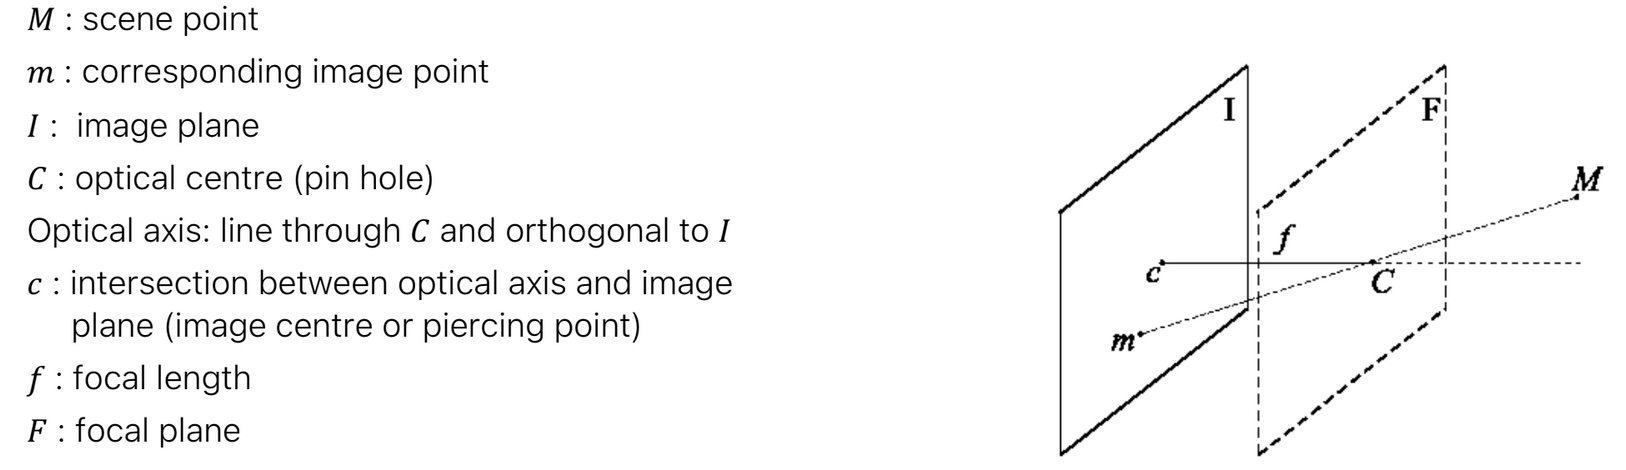
\includegraphics[width=0.9\linewidth]{./img/perspective_projection.jpg}
  \caption{perspective projection}
\end{figure}

Which, by writing the poitns as vectors and the plane's coordinates, becomes the geometric model in the image \ref{fig:perspective_projection_axis}

\begin{figure}[htbp]
  \centering
  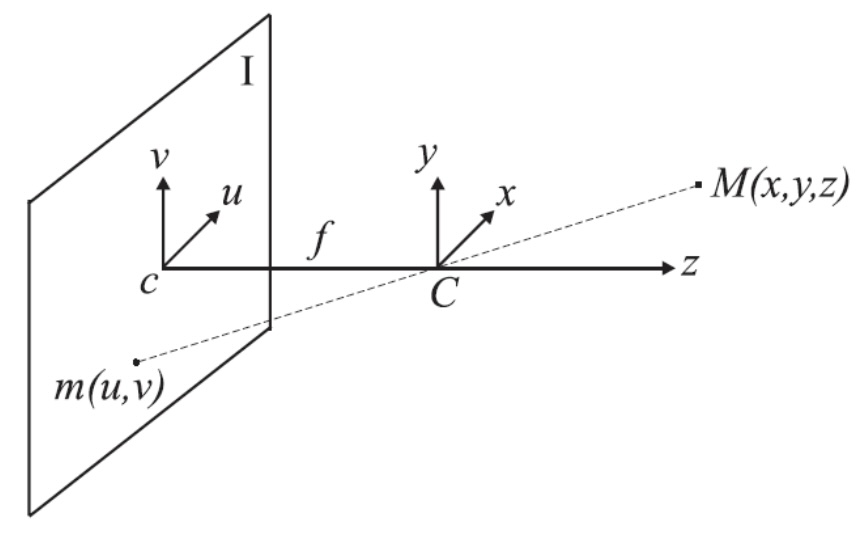
\includegraphics[width=0.45\linewidth]{./img/perspective_projection_axis.jpg}
  \caption{geometric model of image formation}
  \label{fig:perspective_projection_axis}
\end{figure}

Given the reference frame in the image \ref{fig:perspective_projection_axis} 
\begin{itemize}
  \item $u$ is the horizontal axis in the image plane.
  \item $v$ is the vertical axis in the image plane.
  \item $X$ and $Y$ are the respective axis in the 3D reference system. It's called the \textbf{camera reference system} because it is "attached" to the camera.
\end{itemize}

\textbf{For the perspective model these axis must be parallel}

The equations to map scene points into their corresponding image points are defined as:

$$\frac{u}{x} = -\frac{f}{z} \rightarrow u = -x\frac{f}{z} \quad\quad\quad \frac{v}{y} = - \frac{f}{z} \rightarrow v = -y\frac{f}{z}$$

The minus sign means the axis gets inverted (as we can see in the visualization, and it's what happens in the brain).
We can get rid of the sign, since the image plane can be though of as lying in front rather than behind the optical centre.

Image coordinates are a scaled version of scene coordinates (function of depth).
When $z$ increases, since it's at the denominator in both the equations, the terms gets smaller (object gets smaller in the image).
When $f$ increases, since it's at the numerator in both the equations the term gets bigger (object gets bigger in the image)

As we previously said, the image formation process deals with mapping a 3D space onto a 2D space, and so to the loss of depth information.
A given scene point is mapped into an image point, but an image point is mapped onto a 3D line.
For an image point we can only state that its corresponding scene point lays on a line, but cannot disambiguate a specific 3D point along the line.

\subsubsection{Stereo images}

We use multiple images to create stereo vision.
Given correspondences, 3D information can be recovered easily by triangulation.
We can use two cameras, or two cameras and an infrared sensor to project guides to align the images.

For standard stereo geometry there are some assumptions we have to make:
\begin{itemize}
  \item The cameras have parallel $(x,y,z)$ axes.
  \item The image planes of both cameras are coplanar and aligned.
  \item Both cameras have identical focal lengths.
\end{itemize}
\vspace{1em}
Based on this, the transformation between the two reference frames is just a translation, usually horizontal.
For stereo vision is also really important to \textbf{sense two images at the same moment}.

The cameras are displaced at a given quantity $b$ called baseline.
The \textbf{disparity} is the difference between the horizontal coordinates in the left and right images.

\begin{figure}[htbp]
  \centering
  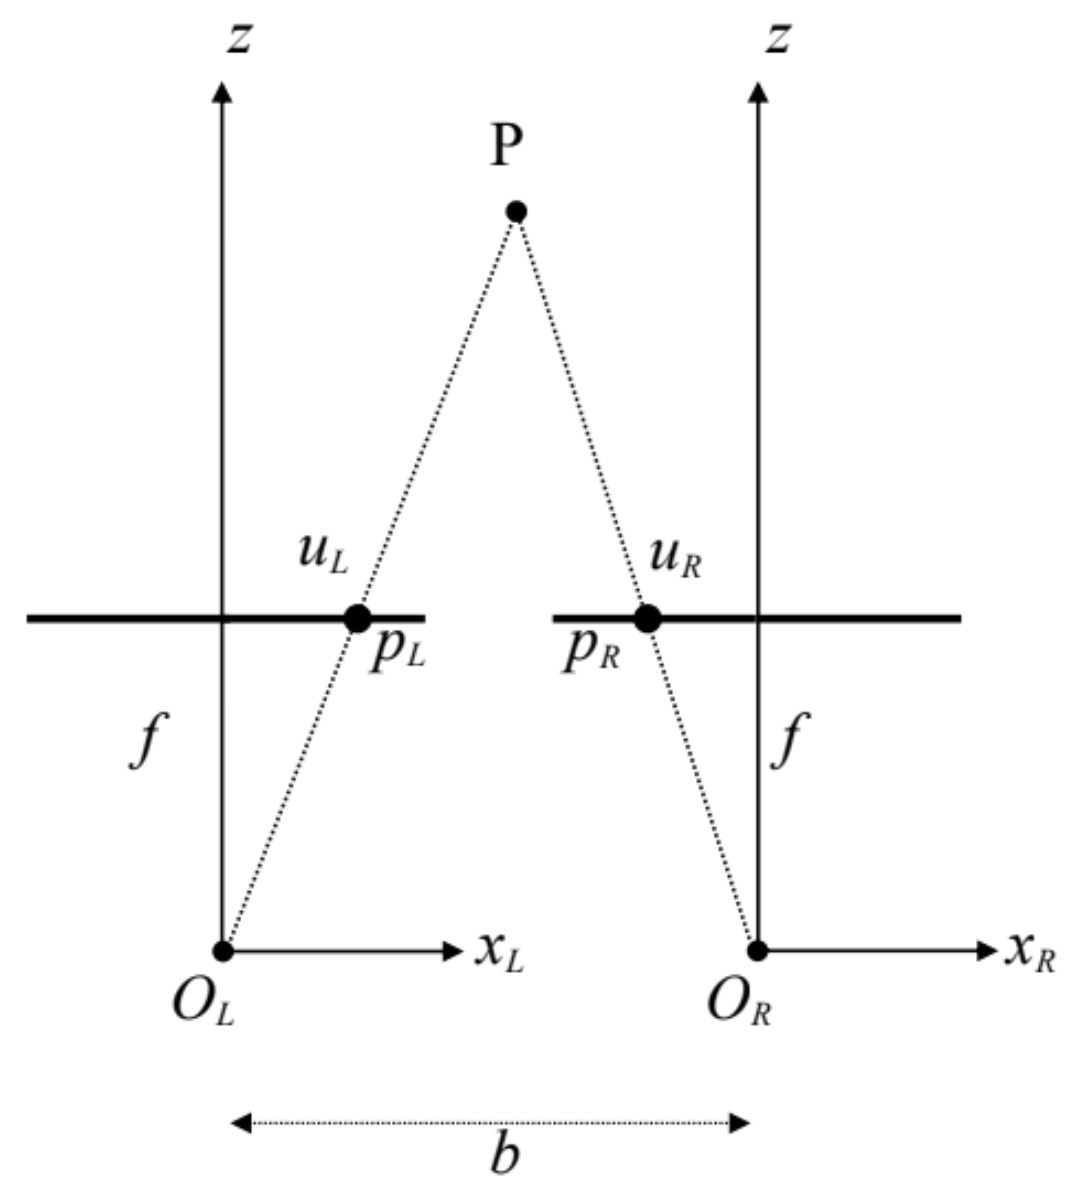
\includegraphics[width=0.45\linewidth]{./img/standard_stereo_geometry.jpg}
  \caption{standard stereo geometry}
  \label{fig:standard_stereo_geometry}
\end{figure}

% The fundamental relationship in stereo vision is $z = b \cdot \frac{f}{d}$.
% It's used to calculate the depth of a point in a scene from a pair of stereo images.

In standard stereo geometry since we are given just two 2D images there is no info about the correspondence between two points in the two images.
We can recall that the camera have parallel axes, and so we know that we can search for the correspondence along the horizontal lines.
This task is called stereo matching.

\subsubsection{Stereo correspondence}
In stereo correspondence, given a point in one image, we have to find it in the other image which is the projection of the same 3D point.
Such image points are called corresponding points.
\textbf{Points farther away have a smaller disparity, while close points have a larger display}.

\begin{figure}[htbp]
  \centering
  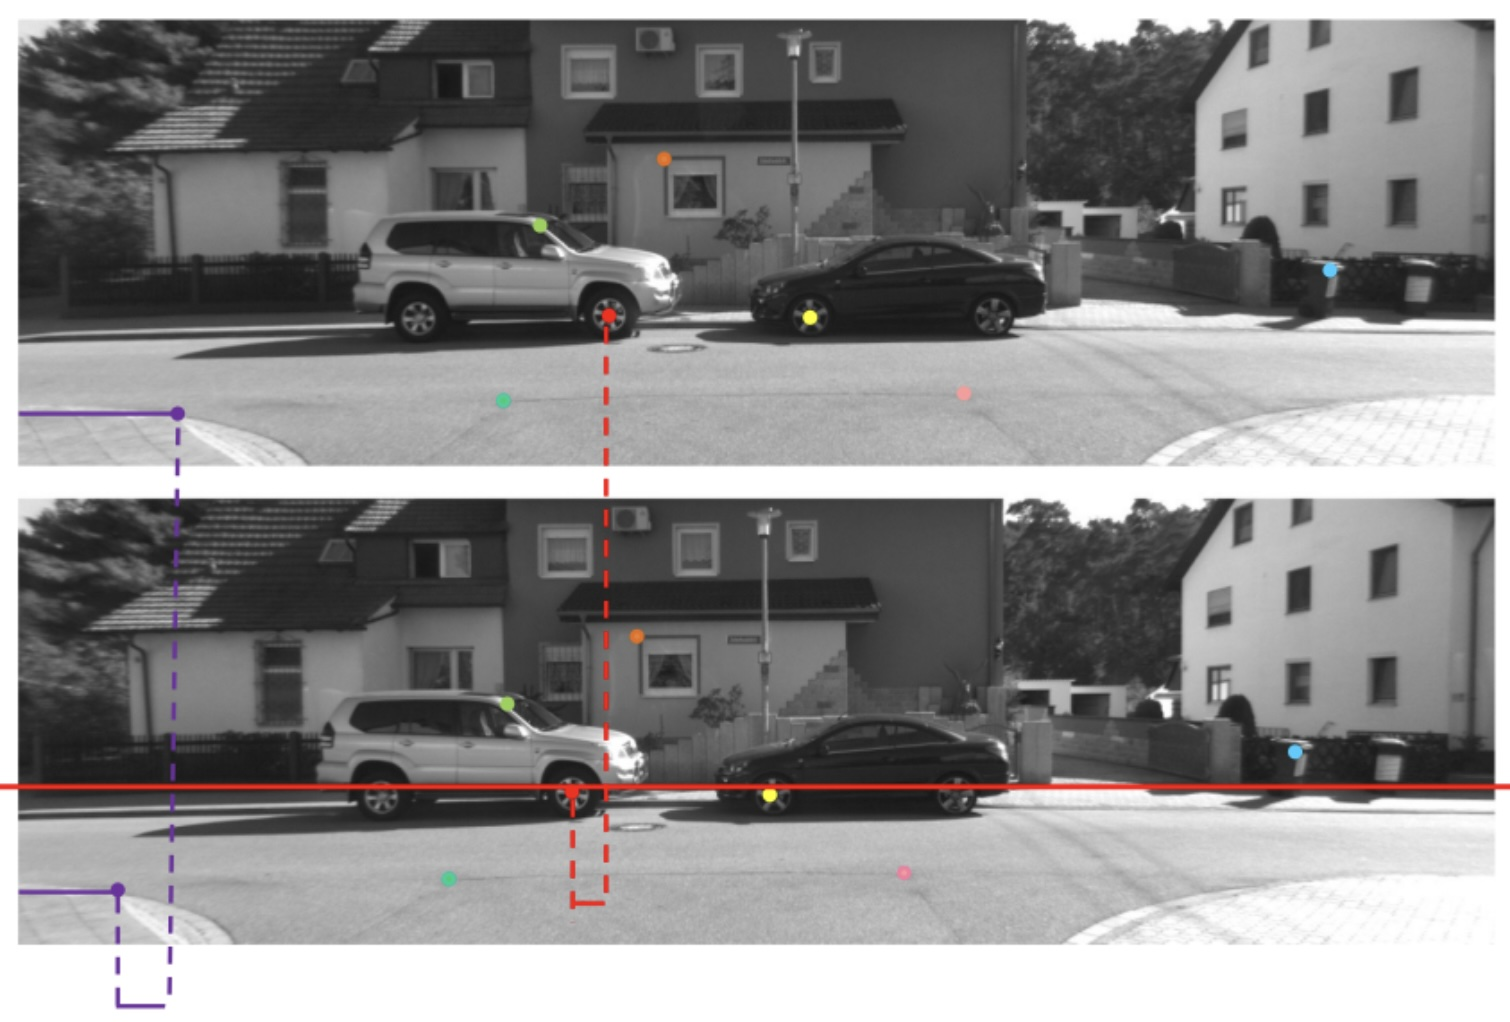
\includegraphics[width=0.65\linewidth]{./img/stereo_correspondence.jpg}
  \caption{Corresponding points look similar in the two images}
  \label{fig:stereo_correspondence}
\end{figure}

The image of a 3D line segment of length $L$ lying in a plane parallel to the image plane at distance $z$ from the optical centre will exhibit a length given by:
$$l = L \frac{f}{z}$$
This relationship is more complicated for an arbitrarily oriented 3D segment, as its position and orientation need to be accounted for as well.
For a \textbf{given position and orientation, length always shrinks alongside distance}.

Perspective projection maps 3D lines into image lines.
\textbf{Parallelism between 3D lines is not preserved} (except for lines parallel to the image plane).
This is the reason why if we look at a really long road into the distance we have the perception that the road becomes thinner, and the lines of the road intersect in the distance.
The images of parallel 3D lines intersect at a point, called \textbf{vanishing point}, which isn't necessarily within the image.

If the lines are parallel to the image plane they meet at infinity.

\subsubsection{Epipolar geometry}

What if the two cameras are no longer aligned? Do we need to search through the whole image?
We can project the line related to point $P_L$ in the right plane and search across that line.
The issue is that this projection can be computed only if the transformation between the two cameras is known (the relative mapping between the two cameras).

\begin{figure}[htbp]
  \centering
  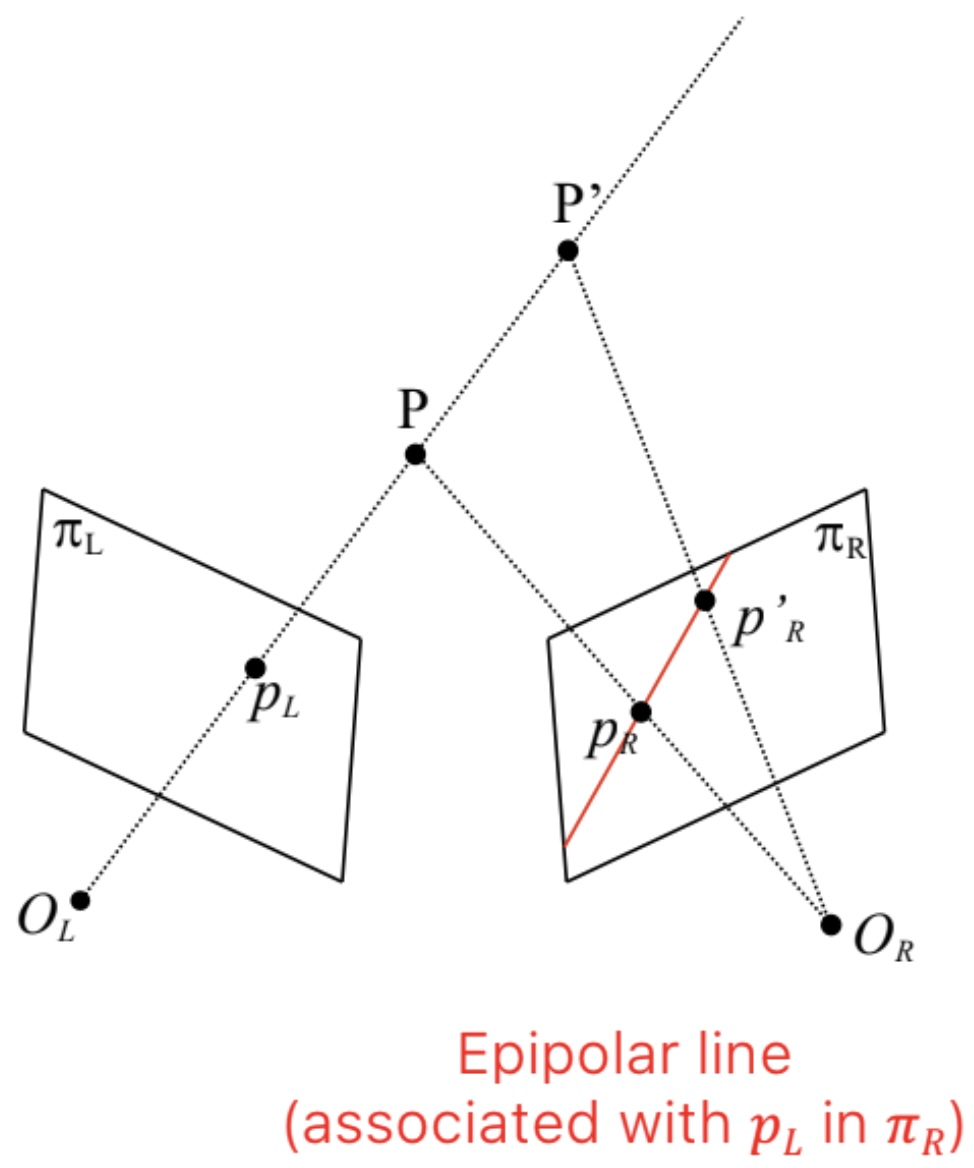
\includegraphics[width=0.45\linewidth]{./img/epipolar_line.jpg}
  \caption{Epipolar line}
  \label{fig:epipolar_line}
\end{figure}

It is almost impossible to build a stereo rig which is perfectly aligned horizontally.
Searching through oblique epipolar lines is awkward, and computationally is less efficient.
What people do in practice is to convert epipolar geometry to standard geometry with rectification/warping.
We warp the images as if they were acquired through a standard geometry, then we can compute and apply to both images a transformation known as rectification.

\subsubsection{Depth of Field (DOF)}

A scene point is on focus when all its light rays, gathered by the camera, hit the image plane at the same point.
In a pinhole device this happens to all scene points because of the very small size of the hole, so that the camera features an infinite Depth of Field (DOF).

The drawback is that such a small aperture allows gathering a very limited amount of light.
The image is really sharp, but has a really low light.
If a point is projected onto a circle instead of a point (bigger pinhole) the image is not sharp (not on focus).
If we cannot gather enough light through the aperture we have to integrate through time, by using a longer exposure time.

\subsubsection{Lenses}

Lenses concentrate light, so we use them to gather more light from a scene point and focus it on a single image point.
This enables much smaller exposure times.
This way Depth Of Field is no longer infinite, and only a limited range of points can be simultaneously on focus in a given image.

We will consider the approximate model known as thin lens equation, which is useful to graphically determine the position of a focused image point:
\begin{itemize}
  \item Rays parallel to the optical axis are deflected to pass through $F$.
  \item Rays through $C$ are undeflected.
\end{itemize}

\textbf{If the image is on focus}, the image formation process obeys to the perspective projection model:
\begin{itemize}
  \item The center of the lens is the optical center.
  \item The distance $v$ acts as the effective focal length of the projection.
\end{itemize}

\begin{figure}[htbp]
  \centering
  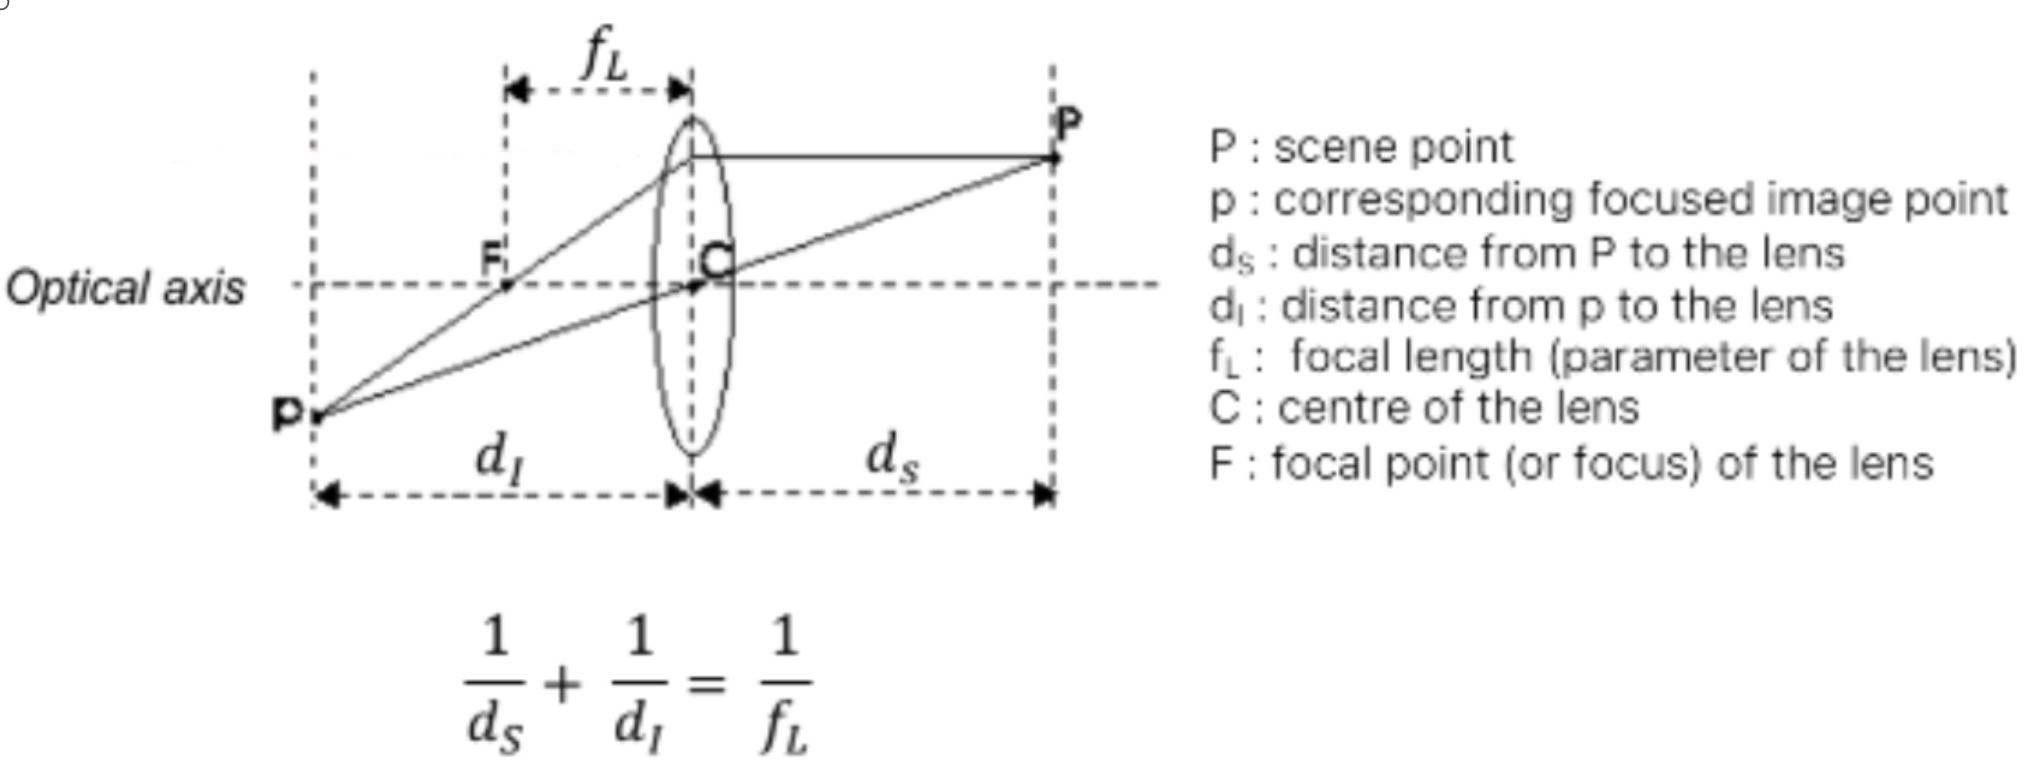
\includegraphics[width=0.7\linewidth]{./img/lens.jpg}
  \caption{Scheme of a lens}
  \label{fig:lens}
\end{figure}

Choosing the distance of the image plane determines the distance at which scene points appear on focus in the image.
Scene points in front and behind the focusing plane will result out-of-focus, thereby appearing in the image as \textbf{blur circles}, rather than points.

The advantage of lenses is to have a small exposure time for capturing moving objects but we pay in terms of Depth Of Field.

\begin{figure}[htbp]
  \centering
  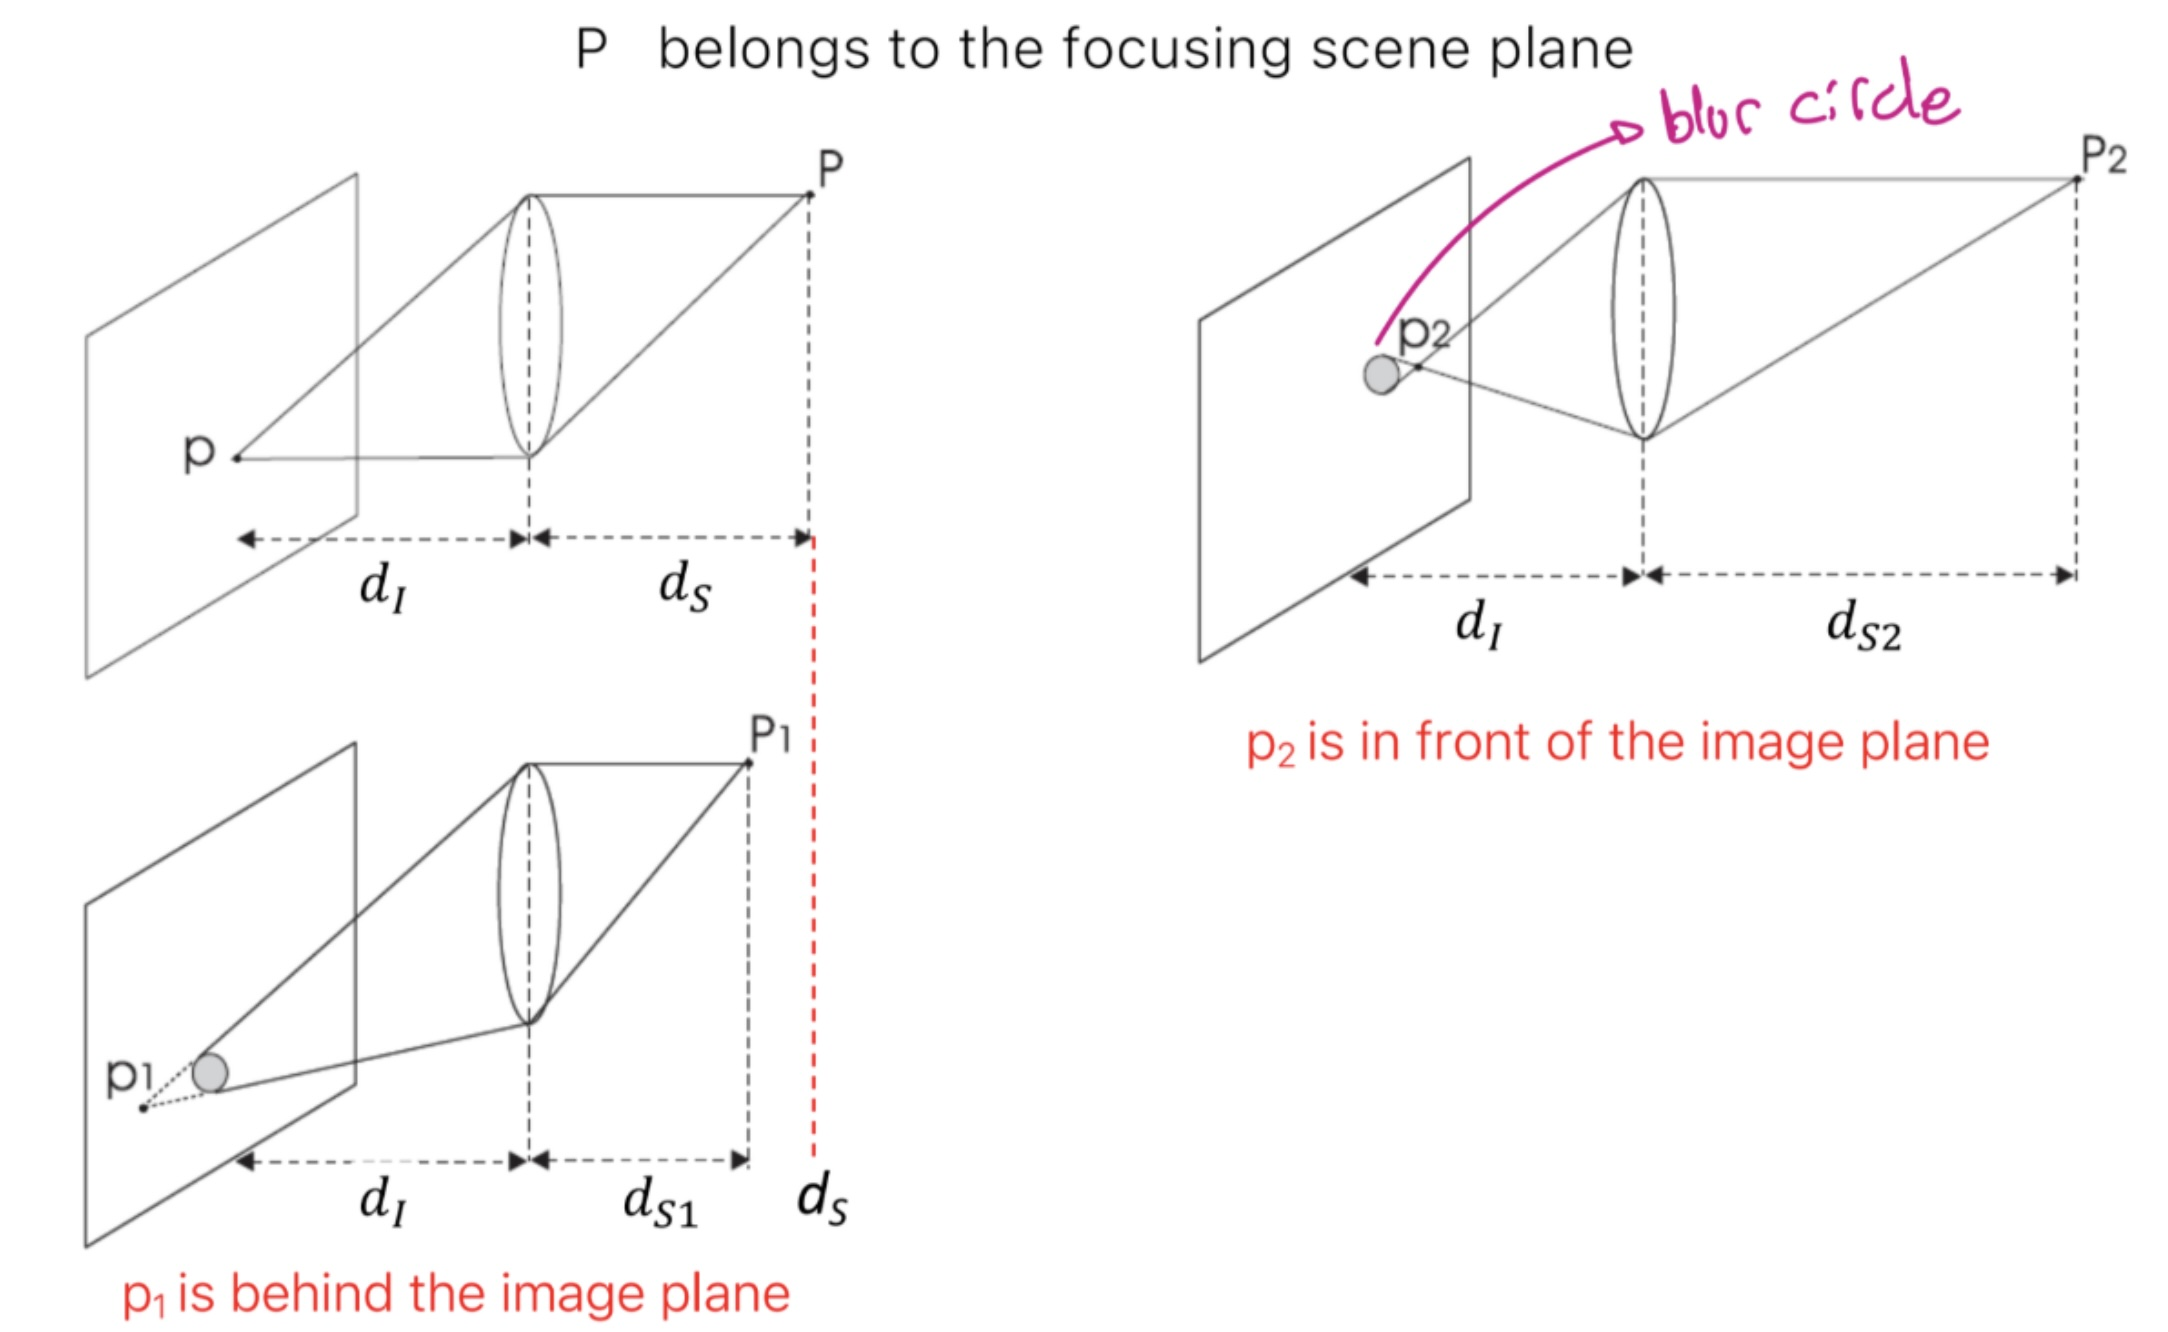
\includegraphics[width=0.8\linewidth]{./img/lens_focus.jpg}
  \caption{Lens focusing at various distances}
  \label{fig:lens_focus}
\end{figure}

As we can see in \ref{fig:tradeoffs} having a small aperture (pinhole camera model) results in everything being on focus, but we need lots of light, or the image will be dark, since few light can enter in the sensor.
We could also increase our exposure time to let more light in, but in that case we need the objects in our image to be still.
Having a bigger aperture results in more light coming in in a small time fraction, but the lens distortion causes the light to be focused only at certain distances, and creates blur cirlces in other zones, so we get a lower depth of field, as we can see in \ref{fig:lens_focus}.

\begin{figure}[htbp]
  \centering
  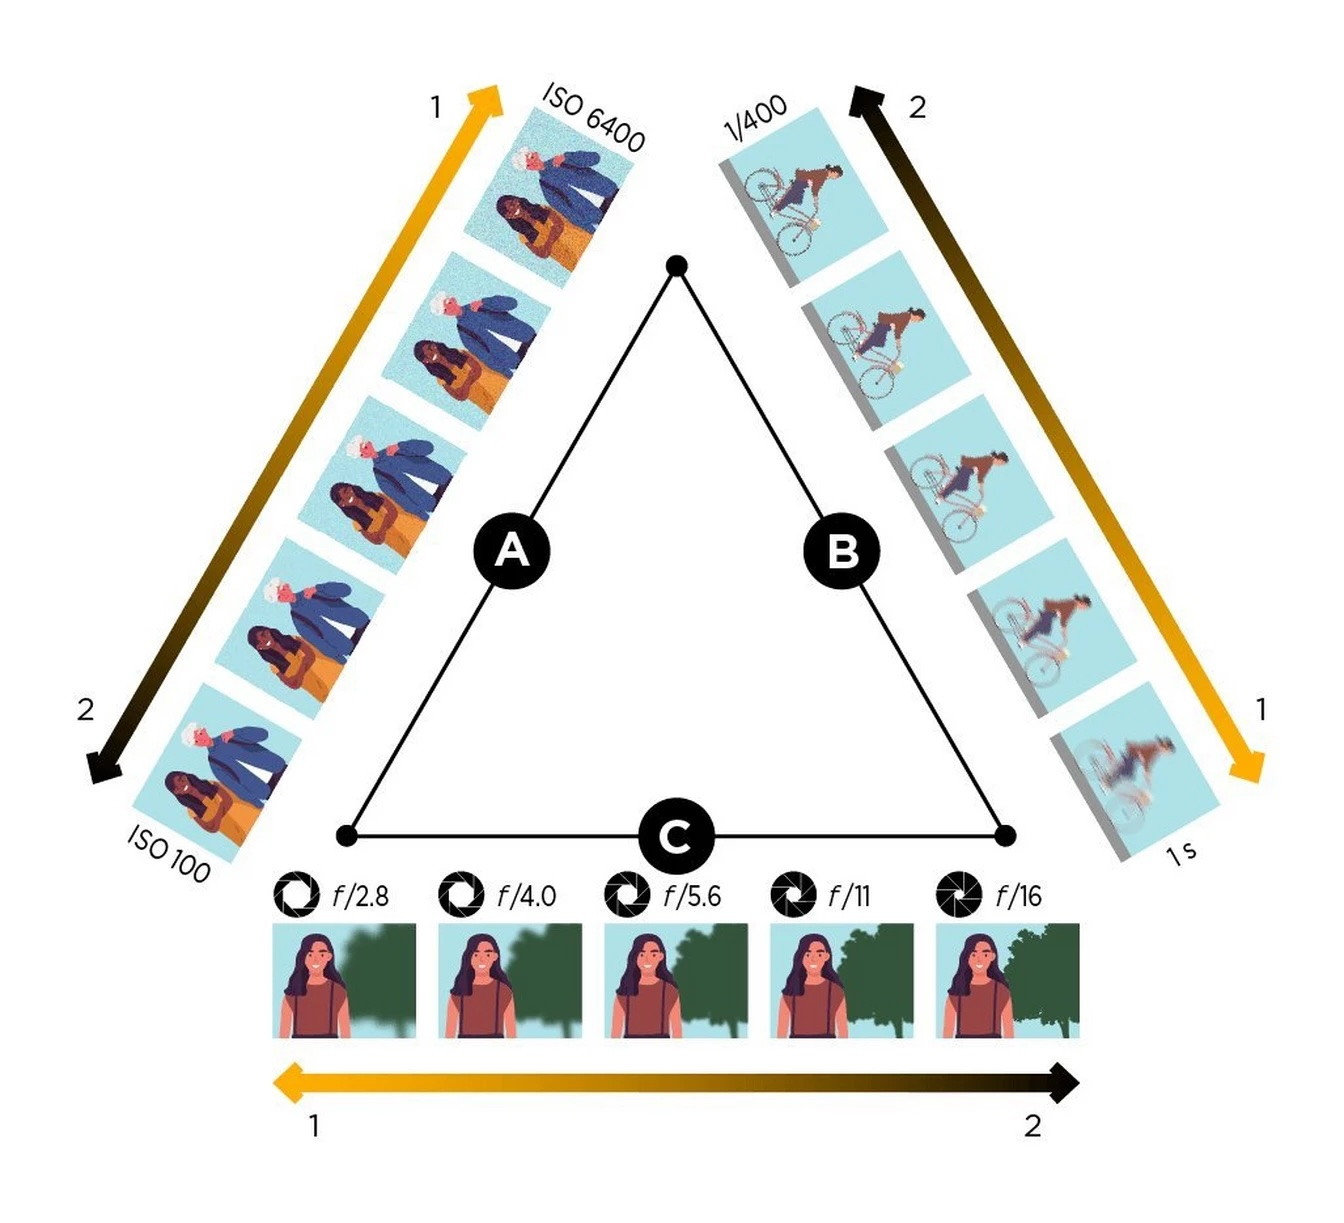
\includegraphics[width=0.8\linewidth]{./img/tradeoffs.jpg}
  \label{fig:tradeoffs}
\end{figure}

\subsubsection{Diaphragm}

In theory, when imaging a scene through a thin lens, only the points at a certain distance can be on focus, all the others appear blurred into circles.
However, as long as the circles are smaller than the size of the photosensing elements (a single pixel), the image will still look on-focus.

\begin{figure}[htbp]
  \centering
  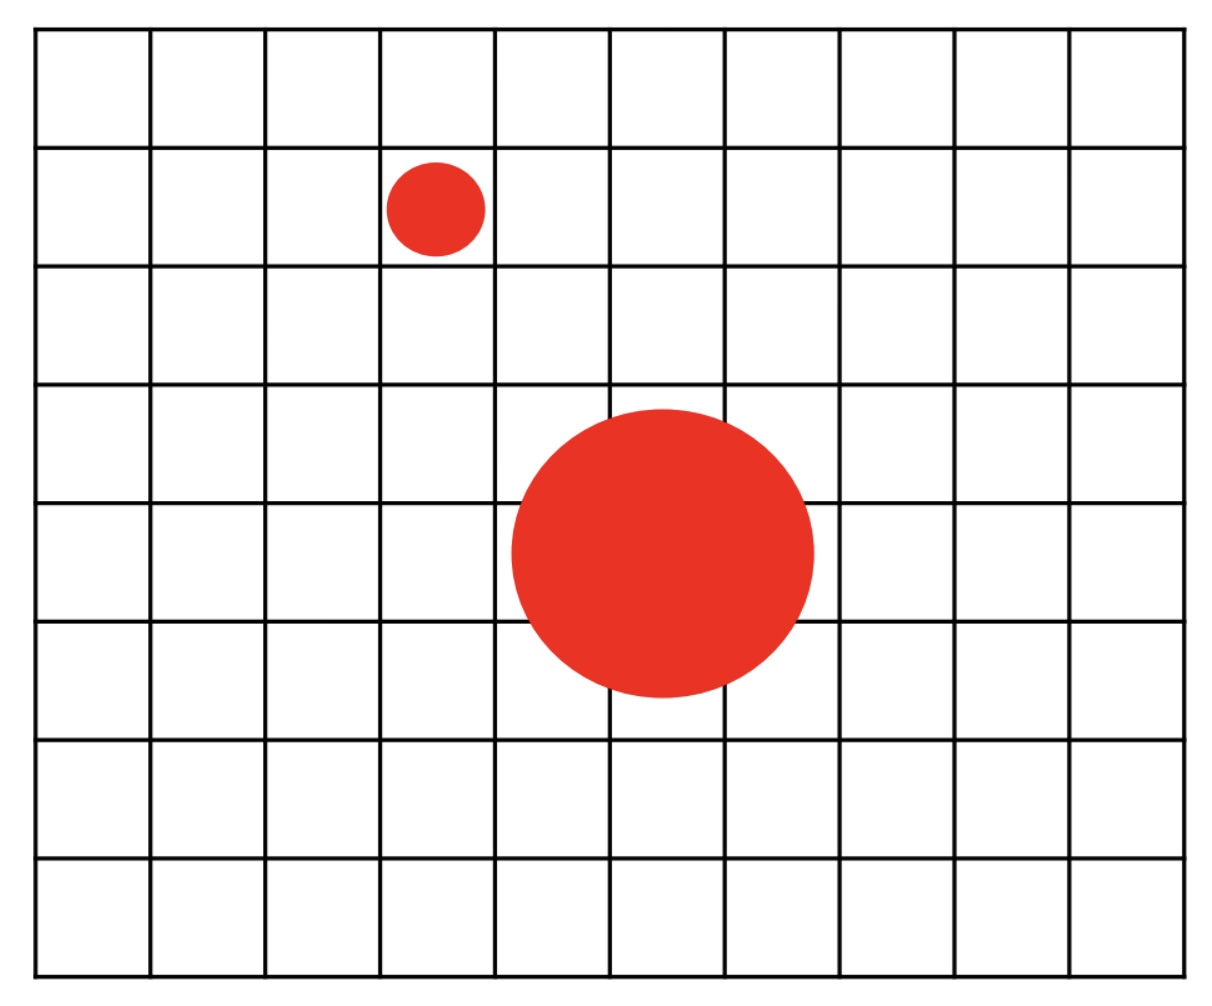
\includegraphics[width=0.55\linewidth]{./img/diaphragm.jpg}
  \caption{Blurring at pixel level}
  \label{fig:diaphragm}
\end{figure}

The range of distances across which the image appears on focus, due to blur circles being small enough, determines the (Depth Of Field) of the imaging apparatus.
Cameras often deploy an adjustable diaphragm (iris) to control the amount of light gathered through the effective aperture of the lens.
\begin{itemize}
  \item Reduce aperture $\rightarrow$ less light $\rightarrow$ smaller blur circle
  \item More aperture $\rightarrow$ more light $\rightarrow$ larger blur circle.
  \item Close the diaphragm $\rightarrow$ increase depth of field $\rightarrow$ not enough light $\rightarrow$ increase exposure time $\rightarrow$ moving object $\rightarrow$ motion blur.
\end{itemize}

\subsubsection{Focusing mechanism (manually changing depth of field)}
To focus on objects at diverse distances we need a mechanism that allows the lens (or the lens subsystem) to translate along the optical axis with respect to the fixed position of the image plane.

\begin{figure}[htbp]
  \centering
  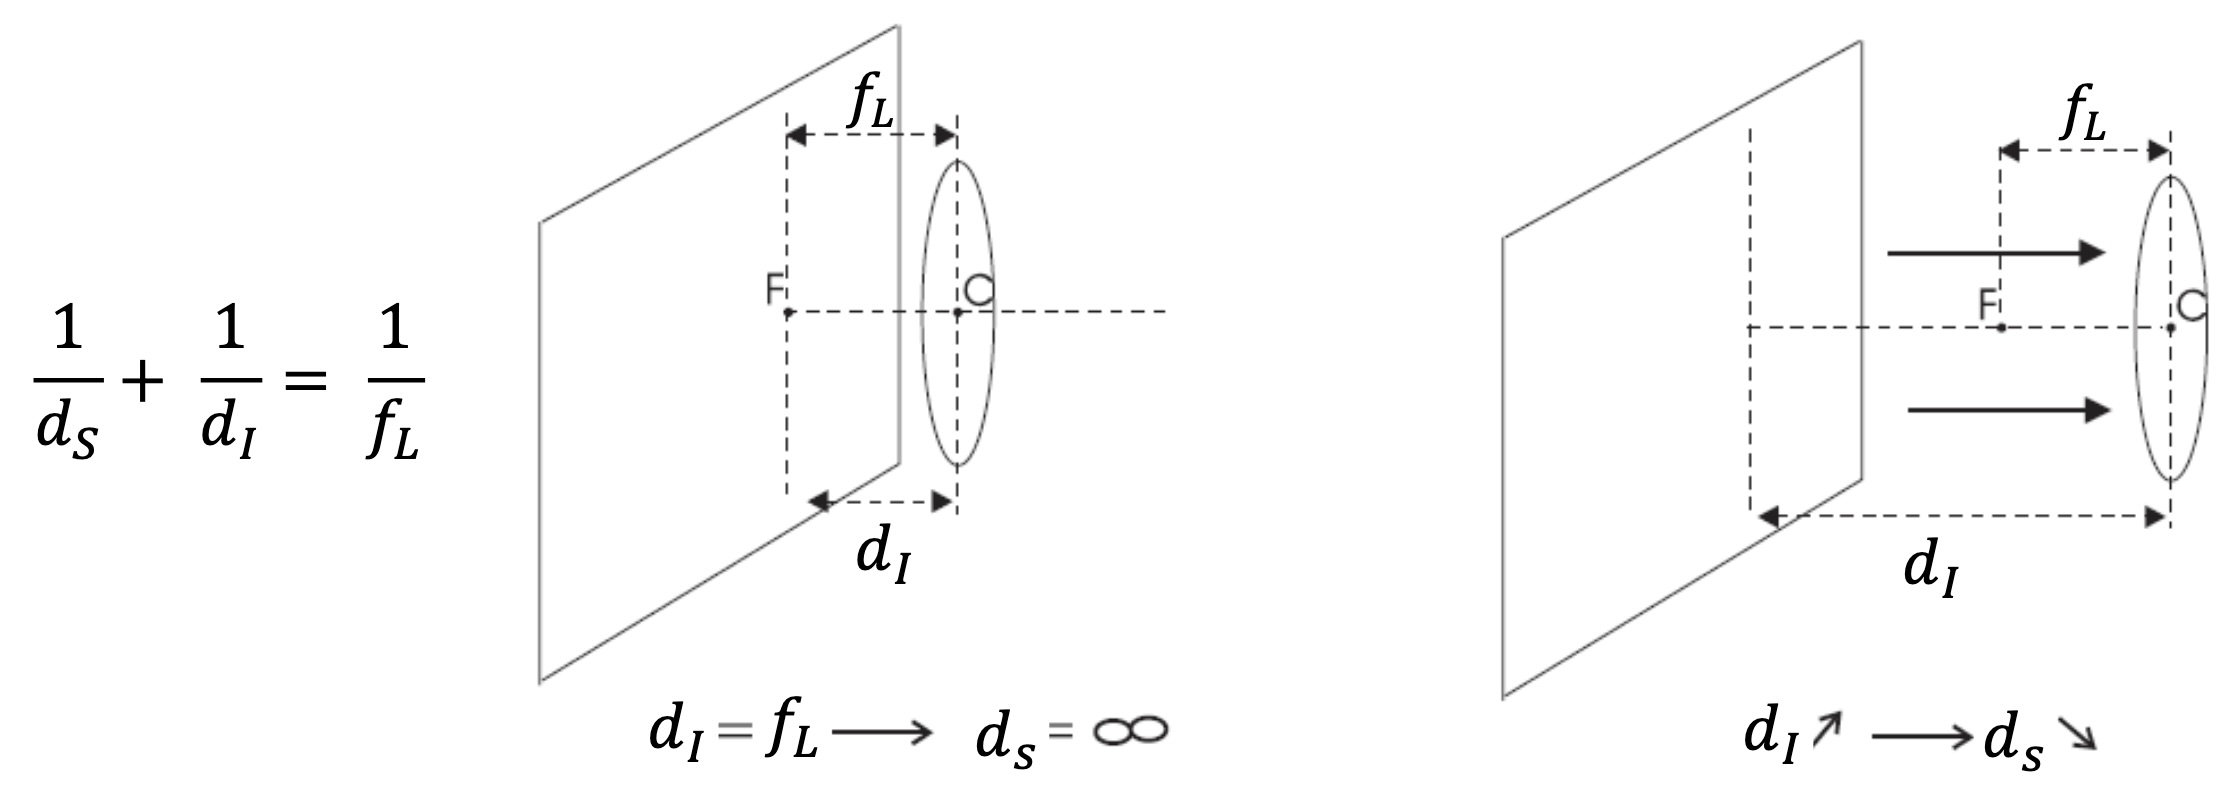
\includegraphics[width=0.7\linewidth]{./img/focusing_mechanism.jpg}
  \caption{Focusing mechanism}
  \label{fig:focusing_mechanism}
\end{figure}

At one end position ($d_I = f_L$) the camera is focused at infinity (objects at inifity are on sharp focus).
The focusing mechanism allows the lens to be translated farther away from the image plane up to a certain maximum value, which determines the minimum focusing distance.

\subsubsection{Image digitization}

How do we convert a continuous image to a discrete one which can be represented on a computer? 
The process can be divided in two steps: sampling and quanitzation.

\begin{figure}[htbp]
  \centering
  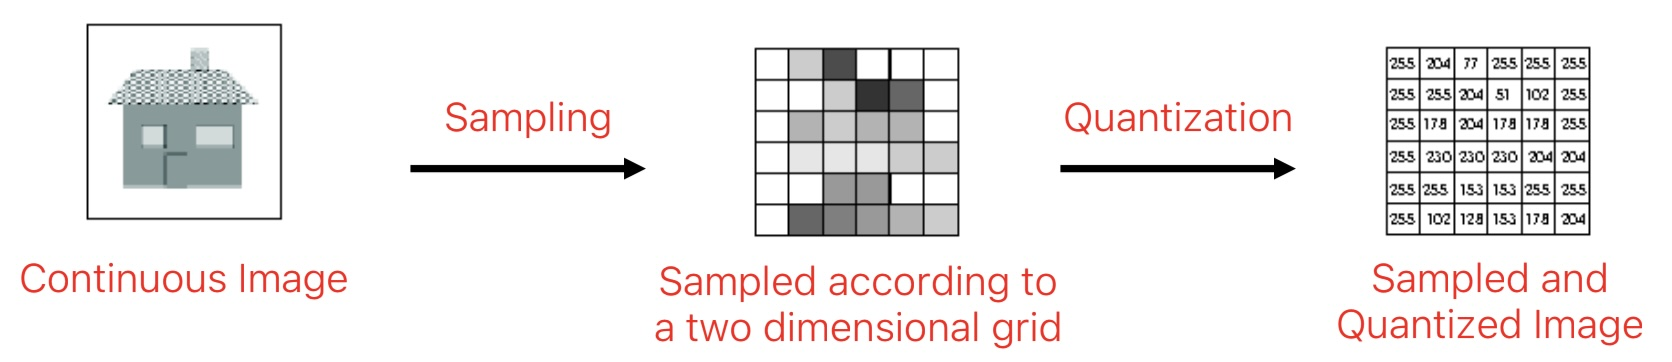
\includegraphics[width=0.55\linewidth]{./img/image_digitization.jpg}
  \caption{The two steps of the image digitization process}
  \label{fig:image_digitization}
\end{figure}

\begin{itemize}
  \item \textbf{Sampling}: the planar continuous image is sampled along both the horizontal and vertical directions to pick up a matrix of $N\times M$ samples (pixels).
  \item \textbf{Quantization}: the continuous range of values associated with pixels is quantized into $l=2^m$ discrete levels known as gray-levels.
  $m$ is the number of bits used to represent a pixel, with the memory occupancy (in bits) of a gray-scale image given by $B = N \times M \times m$. Coloured digital images are typically represented within computers using 3 bytes per pixels. Both more pixels and more bits per pixel result in a higher quality image.
\end{itemize}

The more bits we spend for its representation, the higher the quality of the digital image (it becomes a closer approximation to the ideal continuous image).
This applies both to sampling and quantization.

\subsubsection{Camera sensors}

The sensor is a matrix of photodetectors.
During exposure time, each detector converts the incident light into a proportional electic charge.
The companion circuitry reads-out the charge to generate the output signal, which can be either digital or analog.
For digital cameras the sensor includes the necessary ADC circuitry.

Today, the two main sensor technologies are:
\begin{itemize}
  \item \textbf{Charge Coupled Devices (CCD)}, where the sensor and circuit are separated.
  \item \textbf{ Complementary Metal Oxide Semiconductor (CMOS)}, where everything is on the same circuit.
\end{itemize}

CCD/CMOS sensors can't sense colors, so we place an array of optical filters in front of the photodetectors, to render each pixel sensitive to a specific range of wavelengths.

\subsubsection{SNR}

The intensity measured at a pixel under perfectly static conditions varies due to the presence of random noise.
The main noise sources are:
\begin{itemize}
  \item \textbf{Photon Shot Noise}: the number of photons collected during exposure time is not constant.
  \item \textbf{Electronic Circuitry Noise}: generated by the electronics.
  \item \textbf{Quantization Noise}: related to the ADC conversion.
  \item \textbf{Thermal Noise (Dark Current Noise)}: random charge observed due to thermal excitement.
\end{itemize}

SNR can be expressed both in decibels and bits.

\subsubsection{Dynamic Range (DR)}
If the sensed amount of light is too small, the "true" signal cannot be distinguished from noise.
Given $E_{\text{min}}$: the minimum detectable irradiation, and $E_{\text{max}}$, the saturation irradiation.
The Dynamic Range (DR) of a sensor is defined as $DR = \frac{E_{\text{max}}}{E_{\text{min}}}$, and like the SNR, it is often specified in decibels or bits.

Like SNR, the higher the DR the better it is.
A \textbf{higher DR} corresponds to the ability of the sensor to simultaneously \textbf{capture in one image both the dark and bright} structures of the scene.

% lecture 2 part 2
\subsection{Image Filtering}

\subsubsection{Noise and image filters}

In computer vision we have to deal with noise.
Noise is always different, and more noticeable in uniform regions of the image.
The simplest thing to reduce noise is to output the average of the pixel color over time, to get \textbf{almost} the ideal noiseless value.
$$O(p) = \frac{1}{T} \sum_{t=1}^{T} I_k(p) = \frac{1}{T} \sum_{t=1}^{T}(\tilde{I}(p) + n_t(p))$$

This technique works well on still images.

\begin{figure}[htbp]
  \centering
  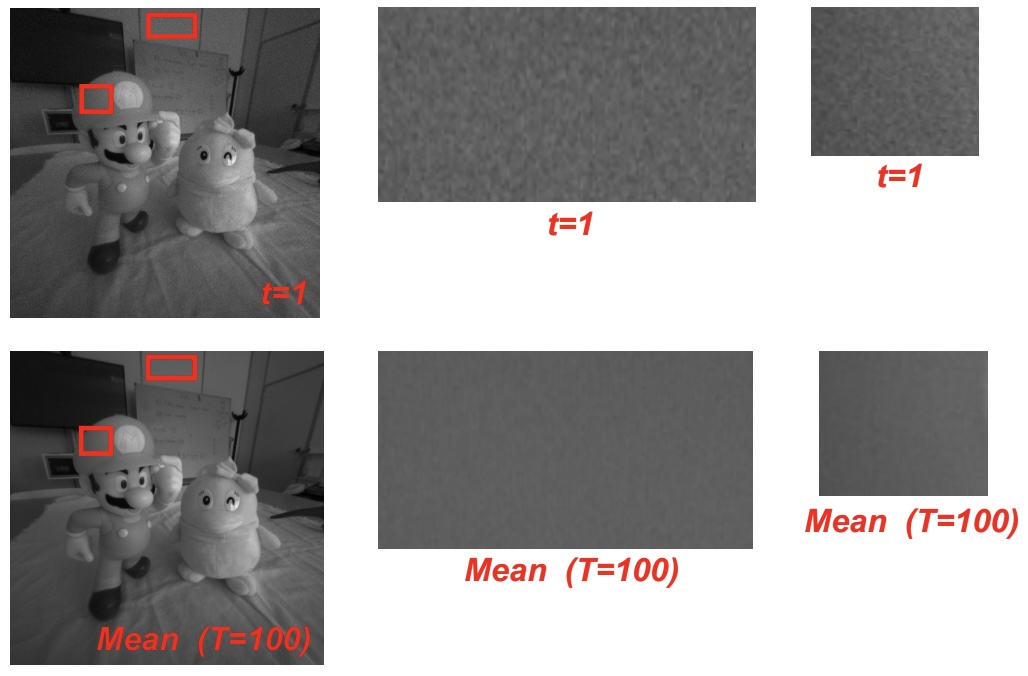
\includegraphics[width=0.7\linewidth]{./img/denoising_simple.jpg}
  \caption{Simple denoising}
  \label{fig:denoising_simple}
\end{figure}

If we are given a simple image, we may compute a mean across neighbouring pixels, like a spatial rather than temporal mean.
The size of the square of the neighbouring pixels is a tradeoff.

This is a very basic denoising filter.

Image filters are image processing operators that compute the new intensity (colour) of a pixel, $p$, based on the intensities (colours) of those belonging to a neighbourhood (support) of $p$.

\subsubsection{Convolution}

An important sub-class of filters is given by \textbf{Linear} and \textbf{Translation-Equivariant (LTE)} operators.

The \textbf{application of filters} in image processing consists in a \textbf{2D convolution} between the input image and the impulse response function of the LTE operator.

LTE operators are used as feature extractors in Convolutional Neural Networks (CNNs).

Given an input 2D signal $i(x,y)$, a 2D operator $T{i(x,y)}$ is said to be linear if and only if
$$ T\{\alpha i_1(x,y) + \beta i_2(x,y)\} = \alpha o_1(x,y) + \beta o_2(x,y) $$ with $o_1 = T{i_1}$ and $o_2 = T{i_2}$ and $\alpha, \beta$ are two constants.
The operator is said to be \textbf{translation-equivariant} if and only if: $T\{i(x-x_0, y-y_0)\} = o(x-x_0, y-y_0)$

If the operator is LTE, the output signal is given by the \textbf{convolution} between the input signal and the impulse response (point spread function) $h(x,y) = T{\delta (x,y)}$.

$$o(x,y) = i(x,y) * h(x,y) = T\{i(x,y)\}$$

$$i(x,y) * h(x,y) = \int_{-\infty}^{\infty} \int_{-\infty}^{\infty} i(\alpha, \beta) h(x-\alpha, y-\beta) \, d\alpha  d\beta $$

\begin{figure}[htbp]
  \centering
  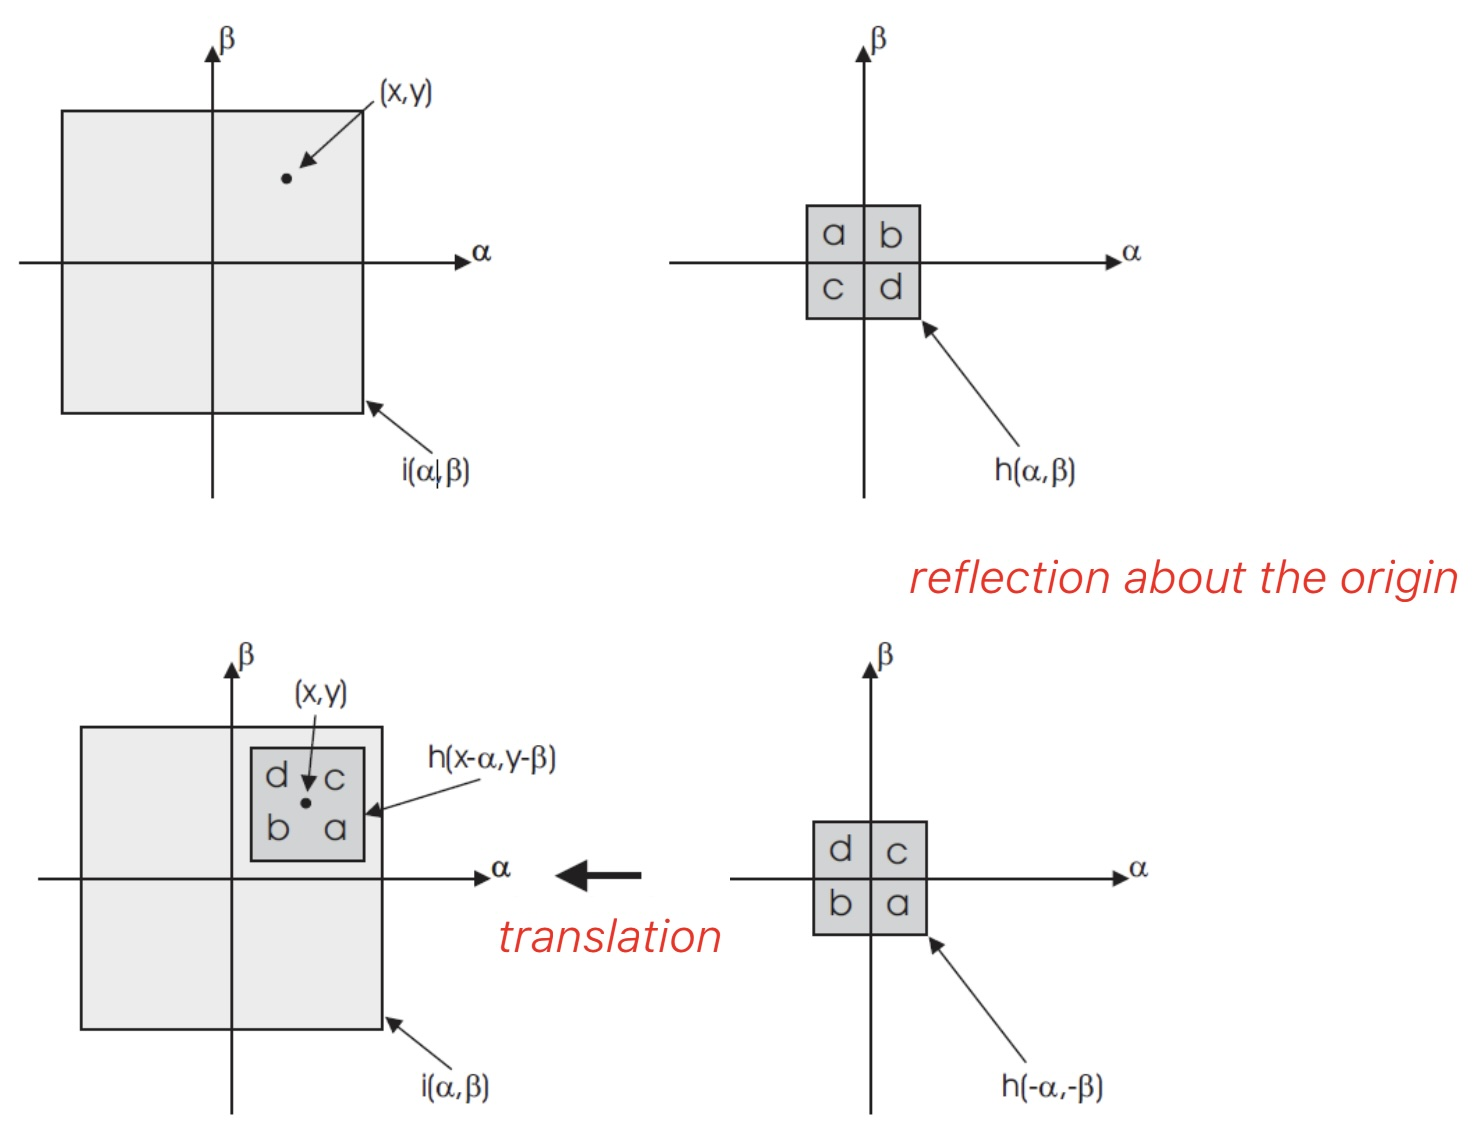
\includegraphics[width=0.6\linewidth]{./img/graphical_convolution.jpg}
  \caption{A graphical view of convolution}
  \label{fig:graphical_convolution}
\end{figure}

Convolutions have some useful properties:
\begin{itemize}
  \item \textbf{Associative property}: $f * (g * h) = (f*g)*h$ (useful because we can decompose kernels and obtain faster operations).
  \item \textbf{Commutative property}: $f*g = g*f$.
  \item \textbf{Distributive property}: $f*(g+h) = f*g + f*h$.
  \item \textbf{Convolution commutes with differentiation}: $(f*g)' = f'*g = f*g'$.
\end{itemize}

The correlation of signal $i(x,y)$  with respect to signal $h(x,y)$ is defined as:
$$i(x,y) \circ h(x,y) = \int_{-\infty}^{\infty} \int_{-\infty}^{\infty} i(\alpha, \beta) h(x-\alpha, y-\beta) \, d\alpha  d\beta $$

Correlation is not commutative, unlike the convolution.

\subsubsection{Discrete convolution}

Normal convolution is useful for signal theory, but we want to have a discrete convolution, where we use summations instead of integrals.
The four convolution properties highlighted for the convolution hold for the discrete one too.

\subsubsection{Practical implementation}
CNNs learn flipped kernels.
In image processing both the the input image and the kernel are stored into matrices of given finite sizes, with the image being much larger than the kernel.
Conceptually, to obtain the output image we need to slide the kernel across the whole input image and compute the convolution at each pixel.

We have an issue on borders, since the kernel "goes out" of the matrix of the image.
We have two main options to solve this issue:
\begin{itemize}
  \item \verb|CROP|: common in image processing.
  \item \verb|PAD|: preferred in CNNs. We can do zero-padding, replicate the first pixel many times, reflect the first $k$ pixels (half of the kernel)...
\end{itemize}

Without padding convolutions shrink the images.

\begin{figure}[htbp]
  \centering
  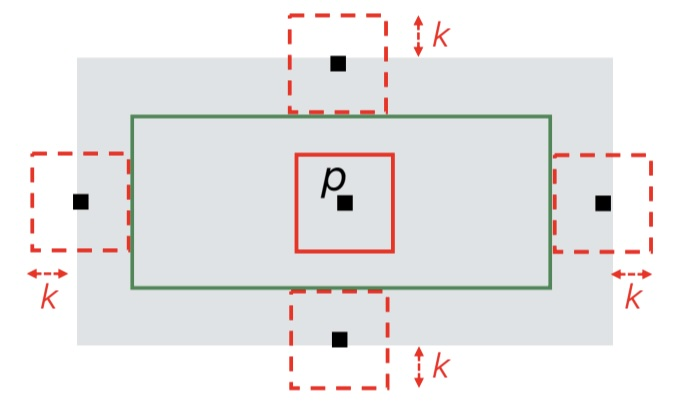
\includegraphics[width=0.7\linewidth]{./img/convolution_visualization.jpg}
  \caption{Issues with convolutions}
  \label{fig:convolution_visualization}
\end{figure}

\subsubsection{Mean filter}

\textbf{Mean filtering} is the \textbf{simplest and fastest way to denoise an image}.
It consists in replacing each pixel intensity by the average intensity overa chosen neighbourhood.
According to signal processing theory, \textbf{the Mean Filter carries out a low-pass filtering operation}, which in image processing is \textbf{also referred to as image smoothing}.
Smoothing is often aimed at image denoising, but sometimes is used to cancel out small-size unwanted details that might hinder the image analysis task.
Linear filtering \textbf{reduces noise but blurs the image}, so we lose sharpness.

% lecture 3
\subsubsection{Gaussian filter}

The Gaussian filter is an LTE operator whose impulse response is a 2D Gaussian function.

\begin{figure}[htbp]
  \centering
  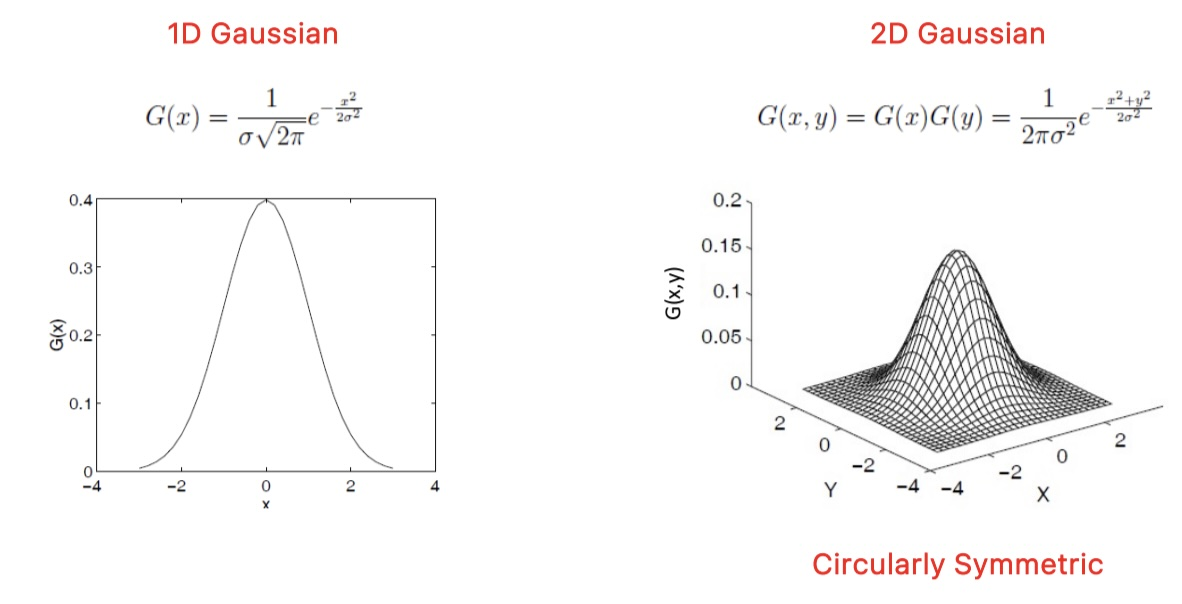
\includegraphics[width=0.7\linewidth]{./img/gaussian_filter.jpg}
  \caption{1D and 2D Gaussian plot}
  \label{fig:gaussian_filter}
\end{figure}

The larger the size of the gaussian kernel, the more accurate the approximation will be, but the computational cost grows with the filter size.
We should then use larger sizes for filters with higher $\sigma$, smaller sizes whenever $\sigma$ is smaller.
A typical rule is to choose the size of the filter by capturing the interval $[-3\sigma, +3\sigma]$ since it captures 99\% of the energy of the Gaussian impulse.
% The Gaussian filter is the only one which has been mathematically proven of not altering image information but just semplification.
To speedup the filtering we can apply the 2D gaussian by doing 2 1D gaussian filterings.

We also observe that the higher the $\sigma$, the higher is the smoothing caused by the filter.
We can use this filter to remove details from the image.

\subsubsection{Median filter}

There is noise that Gaussian filters can't handle well, that is the salt and pepper noise. It's usually caused by image corruption (or broken pixels in the sensor).
Linear filtering is ineffective and just blurs the image.

We can use a \textbf{non-linear filter}, where each pixel intensity is replaced by the \textbf{median over a given neighbourhood}.
Median filtering counteracts impulse noise effectively, since \textbf{outliers tend to fall at either the top or the bottom end of the sorted intensities}.
Median filtering tends to keep sharper edges than linear filters such as the Mean or the Gaussian.

\begin{figure}[htbp]
  \centering
  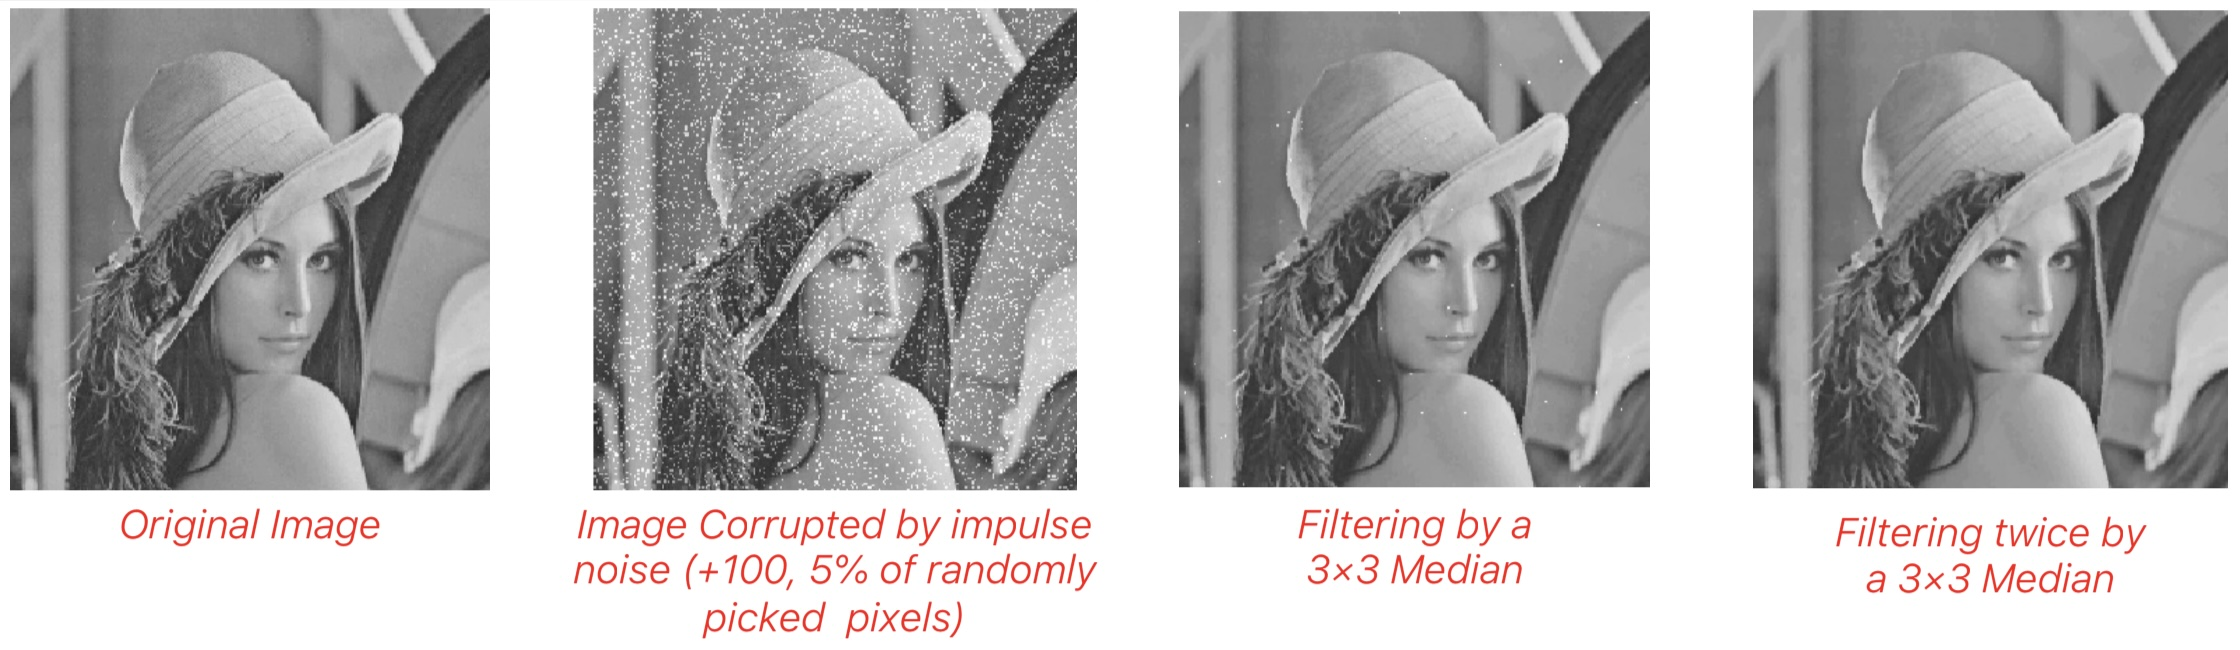
\includegraphics[width=0.9\linewidth]{./img/median_filter_application.jpg}
  \caption{Example of the power of the median filter}
  \label{fig:median_filter_application}
\end{figure}

The median filter can effectively denoise the image without introducing significant blur, yet, Gaussian-like noise, such as sensor noise, cannot be dealt with by the median, as this would require computing new noiseless intensities.

\subsubsection{Bilateral filter}

The bilateral filter preserves edges while filtering out noise.
It's an advanced non-linear filter to accomplish \textbf{denoising of Gaussian-like noise without blurring the image}.
It's also called edge preserving smoothing.

$$O(p) = \sum_{q\in S} H(p,q) \cdot I_q \,\,\,\,\,\,\,\, H(p,q) = \frac{1}{W(p)} G_{\sigma_s}(d_s(p,q))G_{\sigma_r}(d_r(p,q))$$

\begin{itemize}
  \item \textbf{spatial distance}: $d_s(p,q) = ||p-q||_2 = \sqrt{(u_p - u_q)^2 + (v_p - v_q)^2}$.
  \item \textbf{range (intensity) distance}: $d_r(I_p, I_q) = |I_p - I_q|$.
  \item \textbf{normalization factor}: $W(p) = \sum_{q \in S} G_{\sigma_s}(d_s(p,q))G_{\sigma_r}(d_r(p,q))$
\end{itemize}

\begin{figure}[htbp]
  \centering
  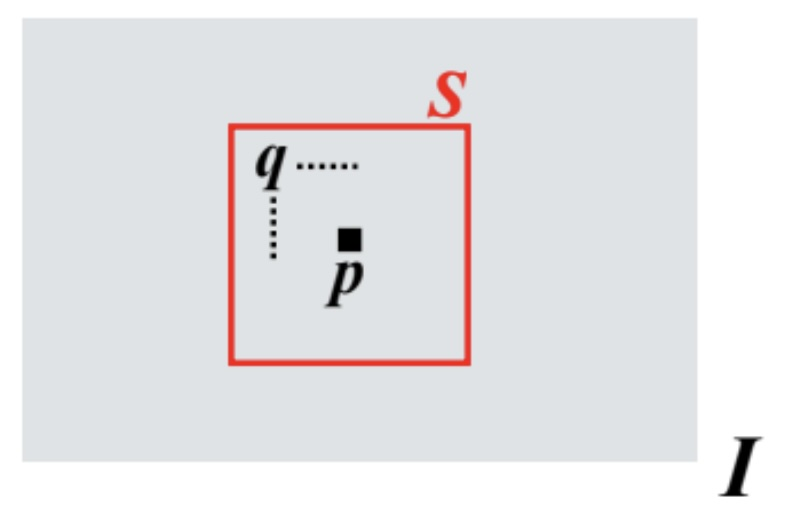
\includegraphics[width=0.5\linewidth]{./img/bilateral_filter_application.jpg}
  \caption{Application of the bilateral filter}
  \label{fig:bilateral_filter_application}
\end{figure}

Given the supporting neighbourhood, neighbouring pixels take a larger weight as they are both closer and more similar to the central pixel.
At a pixel nearby an edge, the neighbourhood falling on the oter side of the edge looks quite different and thus cannot contribute significantly to the output value due to their weights being small.
\textbf{The kernel has to be recomputed for each pixel}.

\begin{figure}[htbp]
  \centering
  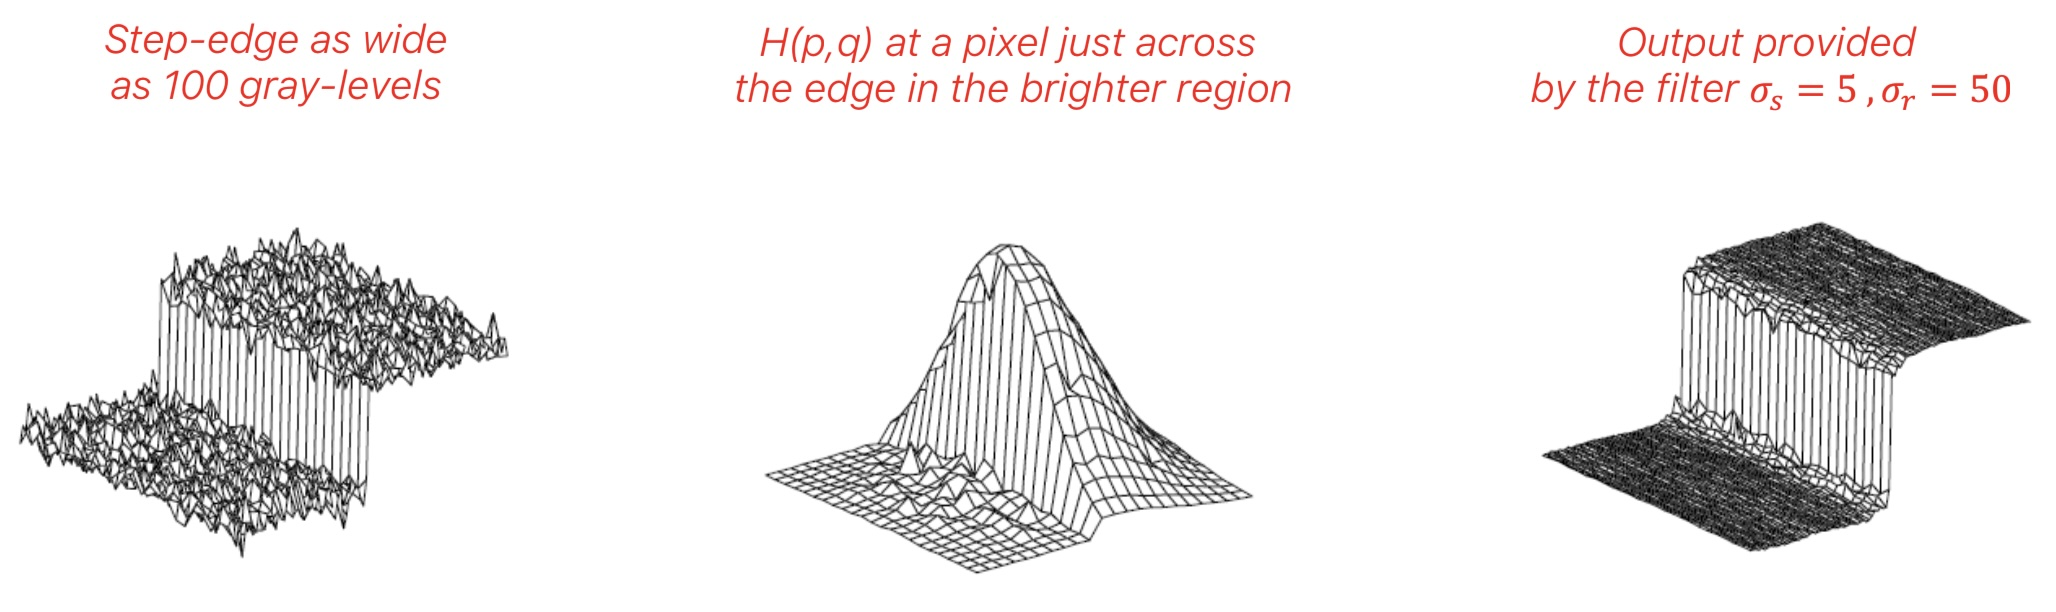
\includegraphics[width=0.9\linewidth]{./img/bilateral_filter.jpg}
  \caption{Bilateral filter differences}
  \label{fig:bilateral_filter}
\end{figure}

\subsubsection{Non-local means filter}

It's another non-linear edge preserving smoothing filter.
The key idea is that the \textbf{similarity among patches spread over the image} can be deployed to achieve denoising.
It's even more expensive than the bilateral filter, since it has to look at more of the image.

\begin{figure}[htbp]
  \centering
  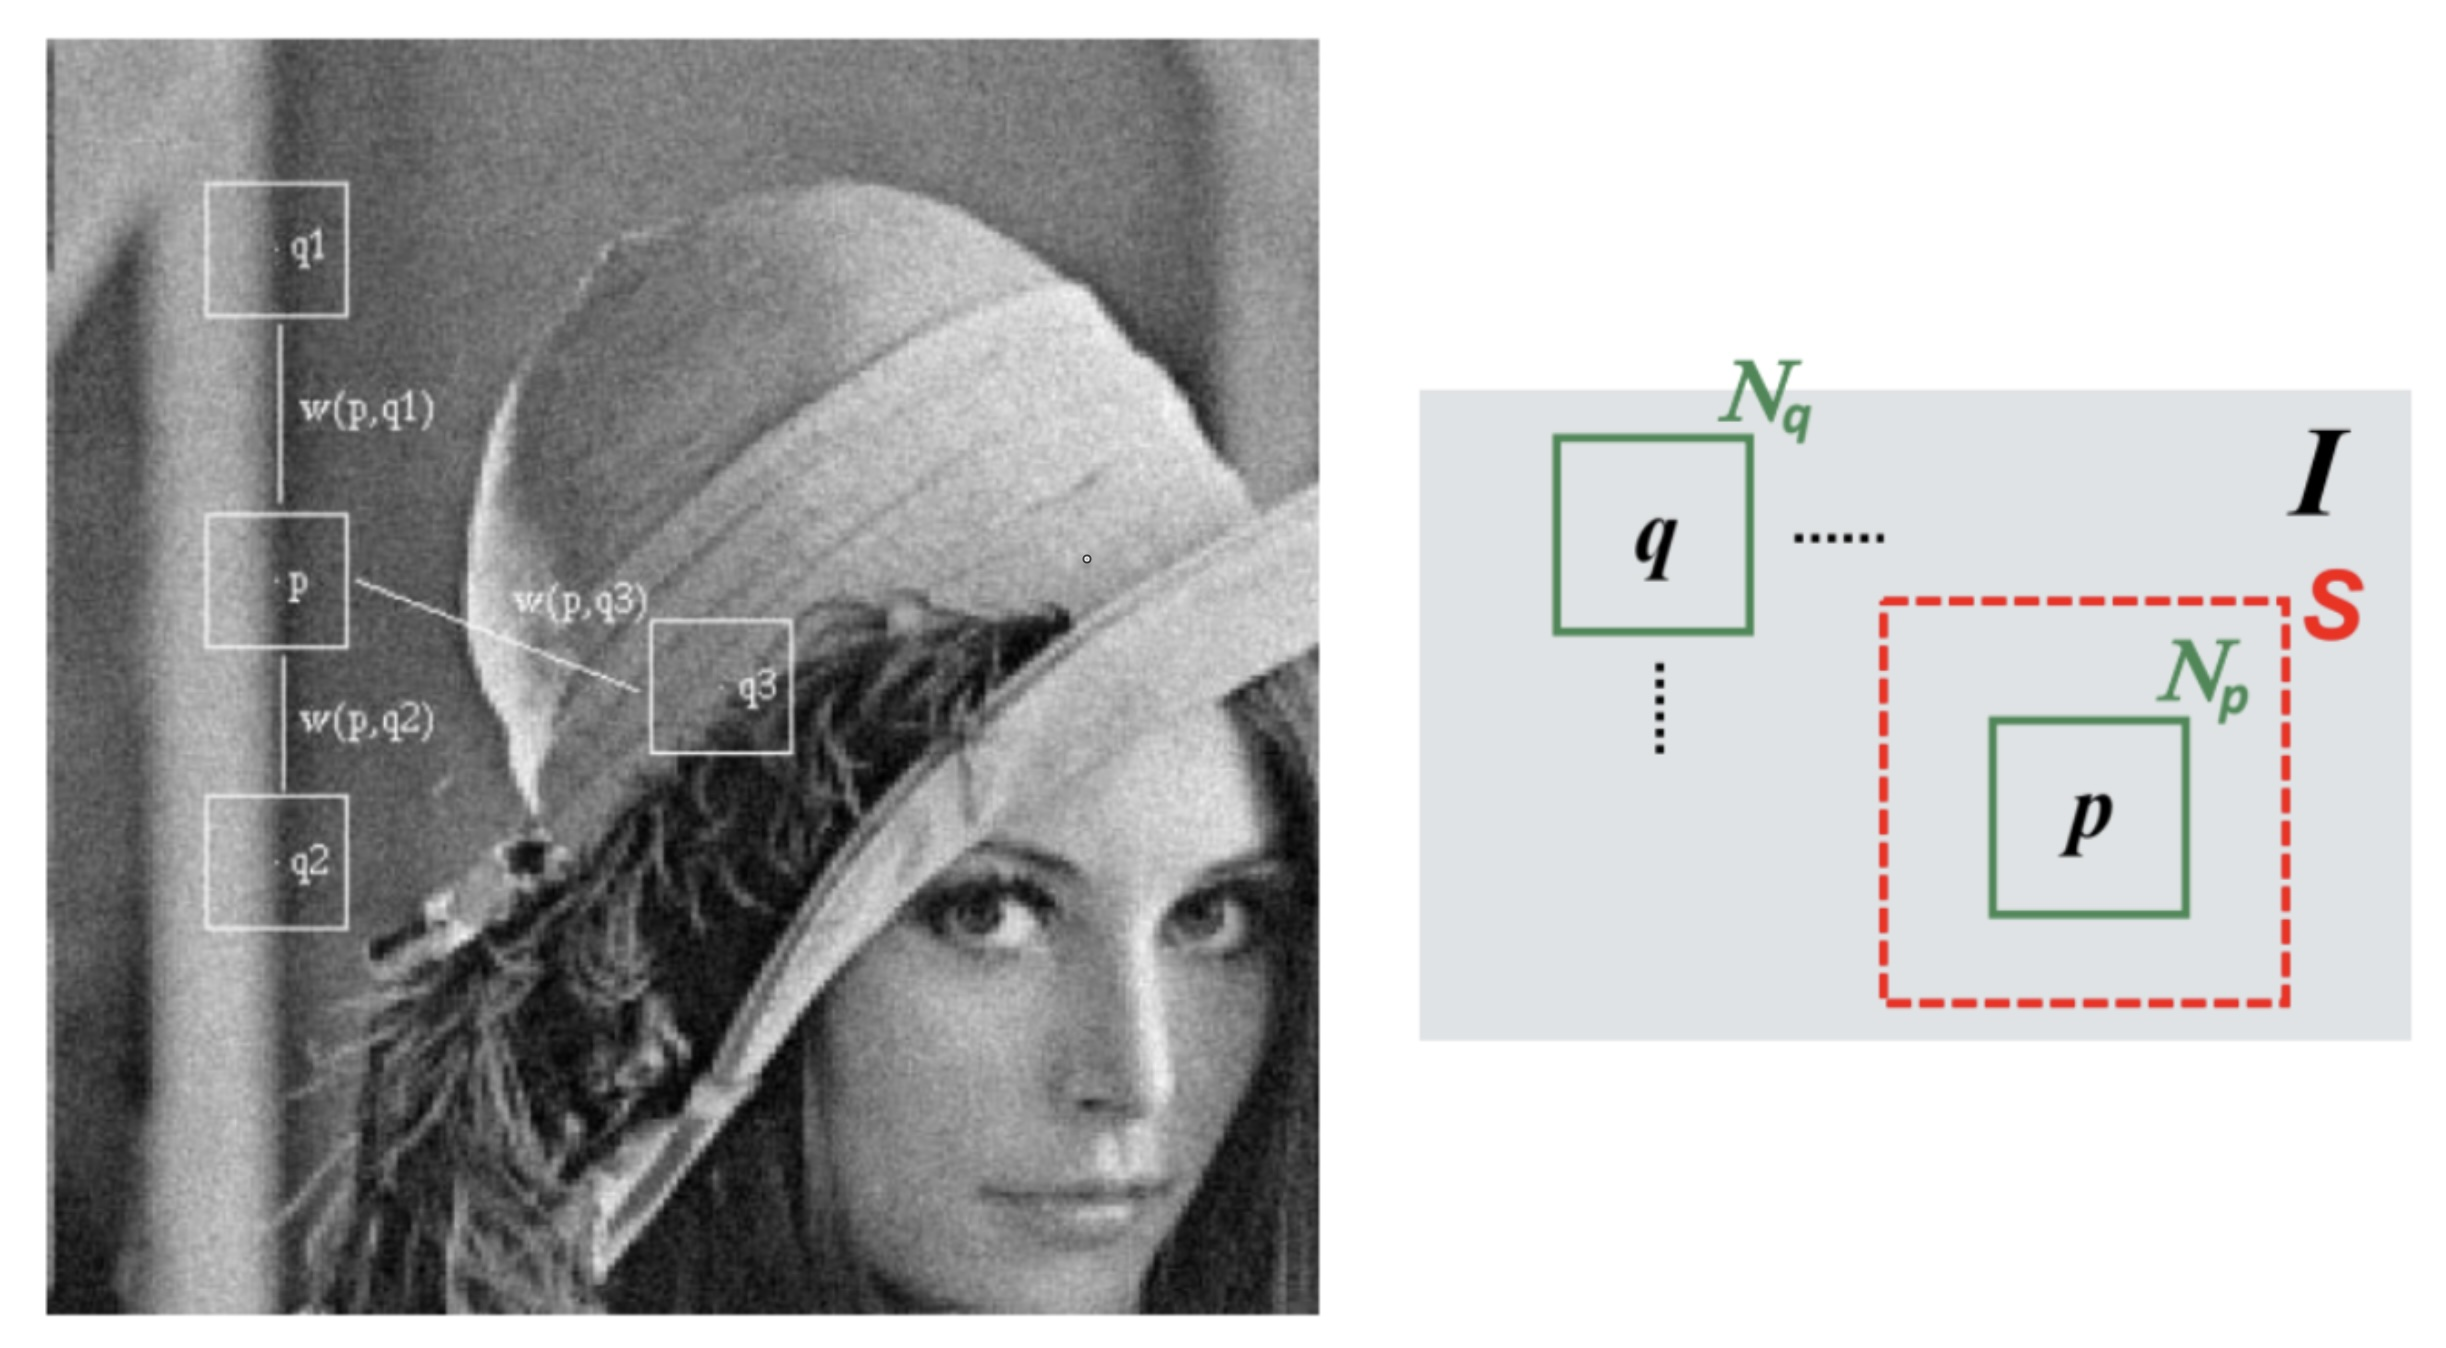
\includegraphics[width=0.7\linewidth]{./img/nonlocalmeans_filter.jpg}
  \caption{Non-local means filter}
  \label{fig:nonlocalmeans_filter}
\end{figure}

\begin{figure}[htbp]
  \centering
  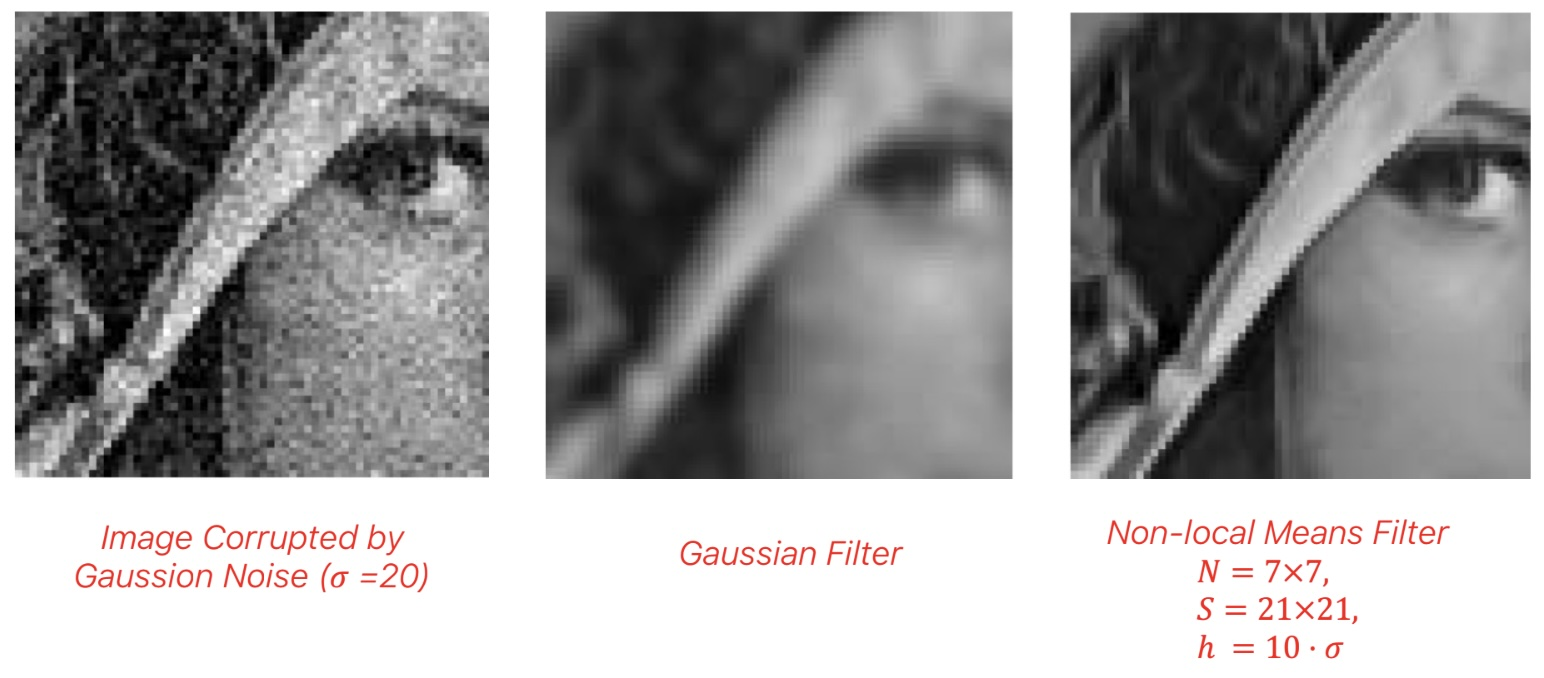
\includegraphics[width=0.7\linewidth]{./img/nonlocalmeans_comparison.jpg}
  \caption{Difference between Gaussian filter and non-local means filter}
  \label{fig:nonlocalmeans_comparison}
\end{figure}

\subsection{Edge detection}

Edge points are local features of the image that capture important information related to its semantic content.
Edges are pixels that lie exactly in between image regions of different intensities.

\paragraph{1D step-edge}
We can detect an edge with a sharp change of a 1D signal (1D step-edge).
The simplest edge-detection operator relies on thresholding the absolute value of the derivative of the signal.

\paragraph{2D step-edge}
A 2D step-edge is characterized not only by its strength but also by its direction (diagonal edge).
The operator which allows us to sense the edge in any direction is the gradient:
$$\nabla I(x,y) = \frac{\partial I(x,y)}{\partial x}i + \frac{\partial I(x,y)}{\partial y}j$$
The \textbf{gradient tells the direction along which the function exhibits its maximum variation}.
We can use differences to approximate the gradient (since we are in the discrete world and we talk about pixels, not functions).
We can estimate the magnitude of the gradient by using different approximations.
We choose $|\nabla I|_{\max}=\max(|I_x|, |I_y|)$, since it's fast and invariant with respect to the edge direction.

\paragraph{Edges and noise}
In real images an edge will not look as smooth as we have seen due to noise.
Taking derivatives of noisy signals is an ill posed problem (the solution is not robust with respect to the input variation) since derivatives amplify noise.
Noise robustness is usually achieved by smoothing the signal before computing the derivatives required to highlight edges.
Smoothing has the side effect of blurring true edges, making it more difficult to detect and localize them, since pixel of different colors will look similar after filtering because of the blending.

\paragraph{Prewitt and Sobel}
% We might wish to approximate partial derivatives by central differences.
% This is done to average around the point because if we are on an edge around us there is a big transition.
% Likewise, the central pixel can be weighted more (the center pixel should be more important).
Prewitt and Sobel address the challenge of detecting edges in noisy environments by combining smoothing and differentiation into a single step.
The Prewitt and Sobel operators perform spatial filtering by using $3 \times 3$ convolution kernels.
Each kernel smooths the image in one direction (reducing noise) and computes the derivative in the perpendicular region (highlighting edges).
Both operators use two kernels: one detects vertical edges, and one horizontal ones.
After convolving the image with both kernels, the gradient magnitude and direction are computed.

$$\text{Magnitude} = \sqrt{G_x^2 + G_y^2} \quad\quad \text{Direction} = \arctan(\frac{G_y}{G_x})$$

Prewitt is better for precise edge localization in cleaner images.
Sobel is preferable in noisy images but may slightly blur edges.


\subsubsection{Non-Maxima Suppression (NMS)}

Detecting edges by gradient thresholding is inherently inaccurate, since \textbf{it's difficult to choose the right threshold} a priori.
A better approach to detect edges may consist in finding the local maxima of the absolute value of the derivative of the signal.

When dealing with 2D images, we should look for:
\begin{itemize}
  \item Maxima of the absolute value of the derivative (gradient magnitude).
  \item Along the gradient direction (orthogonal to the edge direction).
\end{itemize}

We don't know in advance the correct direction to carry out Non-Maxima Suppression (NMS).
The direction has to be estimated locally based on the gradient's direction.
The magnitude of the gradient has to be estimated at points which do not belong to the discrete pixel grid.
Such values can be estimated by linear interpolation of those computed at the closest point belonging to the grid.

A final thresholding step on the magnitude of the gradient at the points selected by the NMS process typically helps pruning out unwanted edges due to either noise or less important details.

\subsubsection{Canny's edge detector}
Canny proposed to set forth quantitative criteria to measure the performance of an edge detector and then to find the optimal filter with respect to such criteria.
The three criteria he proposed were:
\begin{itemize}
  \item \textbf{Good detection}: correctly extract edges in noisy images.
  \item \textbf{Good localization}: distance between found and true edge should be minimum.
  \item \textbf{One response to one edge}: detect one single edge pixel at each true edge.
\end{itemize}

A straightforward Canny edge detector can be achieved by:
\begin{itemize}
  \item Gaussian smoothing.
  \item Gradient computation.
  \item NMS along the gradient direction.
\end{itemize}

2D convolution by a Gaussian can be slow, so we can leverage on separability of the Gaussian function to speedup the calculation: $G(x,y) = G(x)G(y)$.

Non Maxima-Suppression (NMS) is often followed by thresholding of gradient magnitude to help distinguish between true "semantic" edges and unwanted ones.
Edge \textbf{streaking} may occur when magnitude varies along object contours.

Canny proposed a "hysteresis" thresholding approach relying on a higher $T_h$ and a lower $T_l$ threshold.
A pixel is taken as an edge if either the gradient magnitude is higher than $T_h$ or higher than $T_l$ and the pixel is a neighbor of an already detected edge.

The hysteresis thresholding is usually carried out by tracking edge pixels along contours.
First the edge candidates are provided by NMS, then all strong edges are picked, and then for each strong edge we track the weak edges along contours.

\paragraph{Zero-crossing}
Instead of maximum values we can look for zero-crossing of the second derivative of the signal to locate edges (instead of the peaks of the first derivative).
This requires significant computational effort since we are calculating second derivatives.

\subsubsection{Second derivative along the gradient \& Laplacian}
The second derivative along the gradient's direction can be obtained as $n^THn$.

\begin{itemize}
  \item \textbf{Unit vector along the gradient's direction} $n = \frac{\nabla I(x,y)}{||\nabla I(x,y)||}$
  \item \textbf{Hessian matrix} $H =  \begin{bmatrix} \frac{\partial^2 I(x,y)}{\partial x^2} & \frac{\partial^2 I(x,y)}{\partial x \partial y} \\ \frac{\partial^2 I(x,y)}{\partial y \partial x} & \frac{\partial^2 I(x,y)}{\partial x^2} \end{bmatrix} $
\end{itemize}

Computing the second derivative along the gradient turns out very expensive.

\paragraph{Discrete Laplacian}
We can use the forward and backward differences to approximate first and second order derivatives.
It can be shown that the zero-crossing of the Laplacian typically lay close to those of the second derivative along the gradient.
Yet, the former differential operator is much faster to compute.

\subsubsection{Laplacian of Gaussian (LoG)}
A robust edge detector should include a smoothing step to filter out noise.
Edge detection by using the Laplacian of Gaussian (LoG) can be summarized as follows:
\begin{itemize}
  \item \textbf{Gaussian smoothing}: $\tilde{I}(x,y) = I(x,y) * G(x,y)$.
  \item \textbf{Second order differentiation} by the Laplacian.
  \item Extraction of the \textbf{zero-crossing} of $\nabla^2 \tilde{I}(x,y)$
\end{itemize}

Practical implementations of the LoG may deploy the properties of convolutions to speed-up the computation.

We can find sign changes from minus to plus (and viceversa) between two consecutive pixels.
Once a sign change is found, the actual edge may be localized:
\begin{itemize}
  \item At the pixel where the LoG is positive (darker side of the edge)
  \item At the pixel where the LoG is negative (brighter side of the edge)
  \item At the pixel where the \textbf{absolute} value of the LoG is smaller (it's the best choice, since the edge turns out closer to the true zero-crossing).
\end{itemize}

Using a \textbf{higher $\sigma$ yields less details}, so usually we use it for noisy images.

\begin{figure}[htbp]
  \centering
  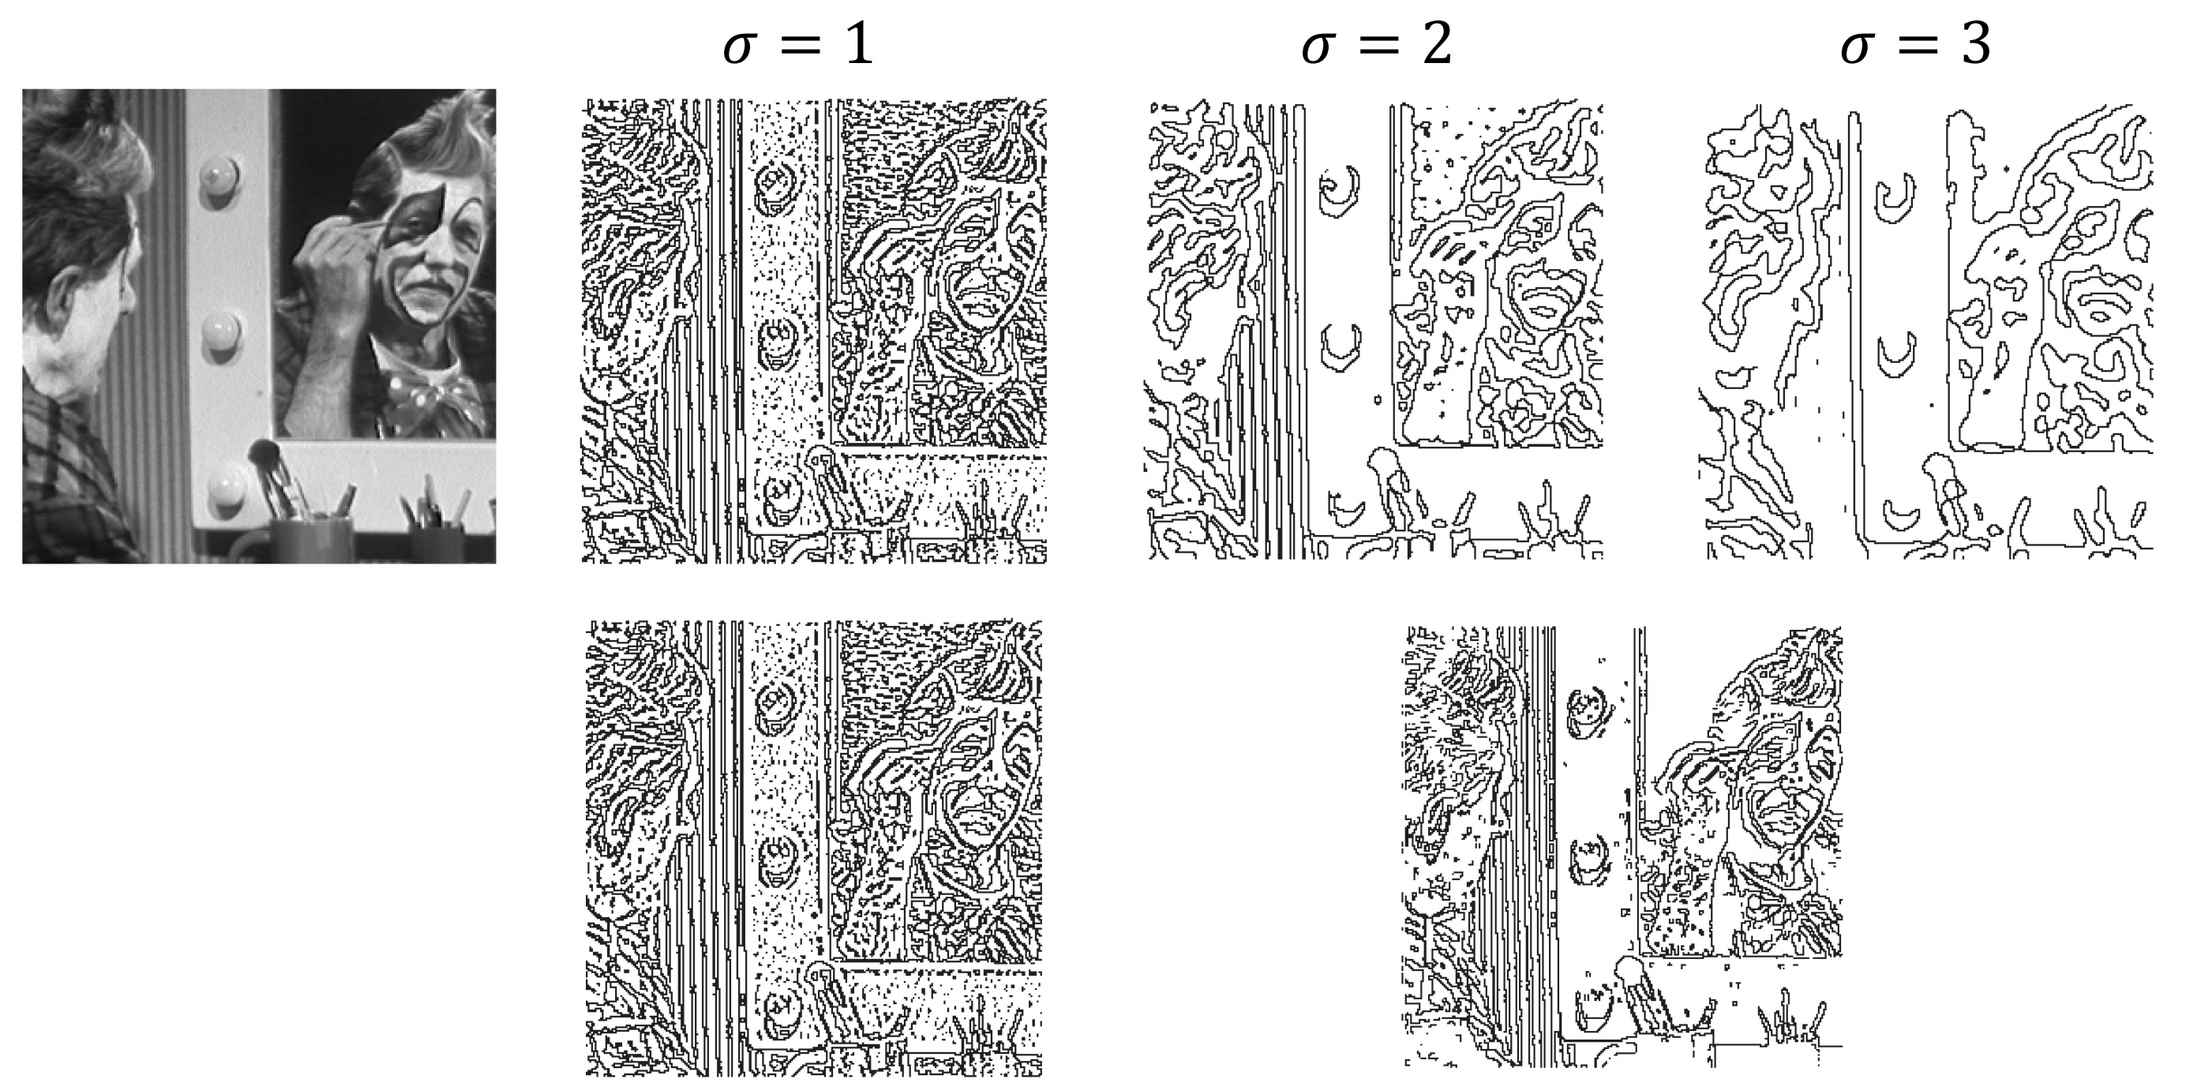
\includegraphics[width=0.7\linewidth]{./img/log_application.jpg}
  \caption{Examples of LoG application}
  \label{fig:log_application}
\end{figure}


\subsection{Feature detection and matching}
Feature detection is useful for object detection, since we can look for features in the source image and try to find them again in the target image.
Several computer vision tasks deal with finding "Corresponding Points" between two (or more) images of a scene.
Correspondences are image points which are the projection of the same 3D point in different views of the scene.
Establishing correspondences may be difficult, as the points may look different in different views.

\subsubsection{Local invariant features paradigm}
The task of establishing correspondences is split into 3 successive steps:
\begin{itemize}
  \item \textbf{Detection} of salient points.
  \item Computation of a \textbf{suitable descriptor} based on pixels in the keypoint neighbourhood.
  \item \textbf{Matching} descriptors between images.
\end{itemize}

Descriptors should be \textbf{invariant} to as many transformations as possible.
Ideally we want scale/rotation/illumination invariance.

\subsubsection{Properties of good detectors/descriptors}
\begin{itemize}
  \item Detector:
  \begin{itemize}
    \item Repeatability: it should find the same keypoints in different views of the scene despite the transformations.
    \item Saliency: it should find keypoints surrounded by informative patterns.
  \end{itemize}
  \item Descriptor:
  \begin{itemize}
    \item Distinctiveness vs. robustness trade-off: the algorithm should capture the salient information around a keypoint.
    \item Compactness: the description should be as concise as possible.
  \end{itemize}
\end{itemize}

Speed is desirable for both, and in particular for detectors, which need to be run on the whole image (while descriptors are computed at keypoints only).

Edge pixels can be hardly told apart as they look very similar along the direction perpendicular to the gradient.
Edges are locally ambiguous, since there are many other points that look just the same.

\subsubsection{Moravec Interest Point Detector}
We can define the \textbf{cornerness} at a point $p$, which is given by the minimum squared difference between the patch centered at $p$ and those centered at its 8 neighbours: 
$$C(p) = \min_{q \in n_8(p)} ||N(p) - N(q)||^2$$

\begin{figure}[htbp]
  \centering
  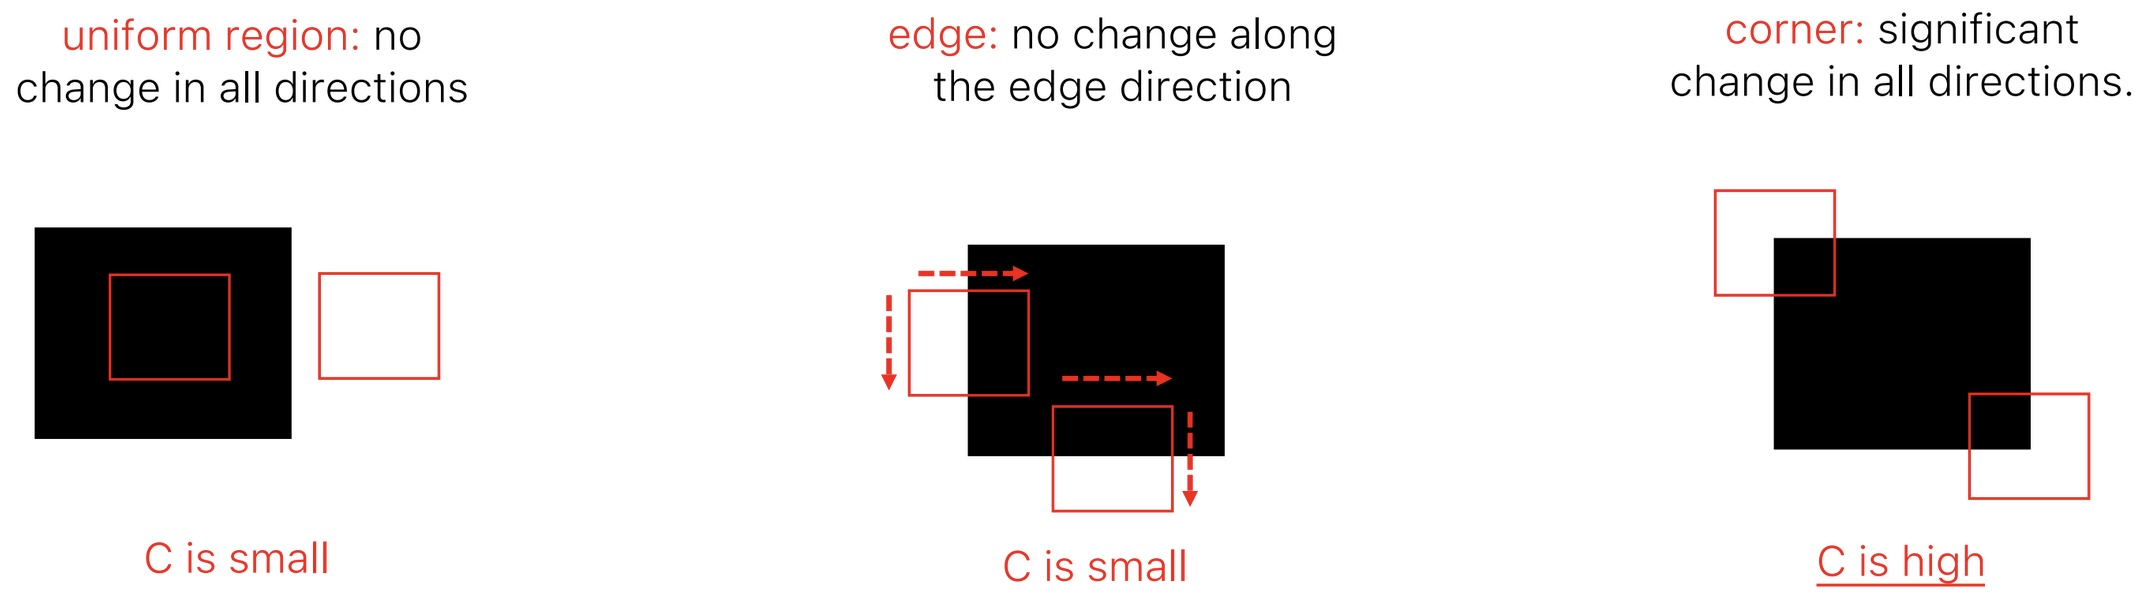
\includegraphics[width=0.9\linewidth]{./img/cornerness.jpg}
  \caption{Cornerness of an image segment}
  \label{fig:cornerness}
\end{figure}

After computing the cornerness we threshold and do Non-Maxima Suppression.

\subsubsection{Harris Corner Detector}

Harris \& Stephens proposed to rely on a continuous formulation of the Moravec's "error" function.
Assume to shift the image with a generic infinitesimal shift $(\Delta x, \Delta y)$:
$w(x,y)$ is a window set to 1 around the pixel under evaluation and 0 in all the image.
In the end we consider only the pixel around the $(x,y)$ position.

Due to the shift being infinitesimal, we can deploy Taylor's expansion of the intensity function at $(x,y)$ : $f(x + \Delta x) = f(x) + f'(x) \Delta x$

$M$ encodes the local image structure around the considered pixel.
We hypothesize that $M$ is a diagonal matrix
$M =
\begin{bmatrix}
\sum_{x,y} w(x,y) I_x(x,y)^2 & \sum_{x,y} w(x,y) I_x(x,y) I_y(x,y) \\
\sum_{x,y} w(x,y) I_y(x,y) I_x(x,y) & \sum_{x,y} w(x,y) I_y(x,y)^2
\end{bmatrix}
=
\begin{bmatrix}
\lambda_1 & 0 \\
0 & \lambda_2
\end{bmatrix}$

\begin{figure}[htbp]
  \centering
  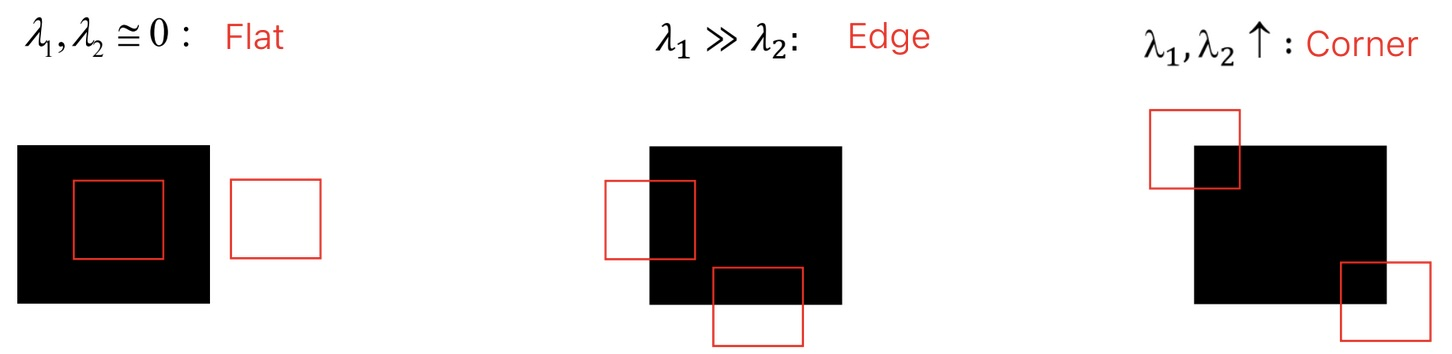
\includegraphics[width=0.9\linewidth]{./img/harris_corner_detector.jpg}
  \caption{Harris corner detector and lambda values}
  \label{fig:harris_corner_detector}
\end{figure}

The previous considerations have general validity as $M$ is real and symmatric, and thus can always be diagonalized by a rotation of the image coordinate system.
$$M = R\begin{bmatrix} \lambda_1 & 0 \\ 0 & \lambda_2 \end{bmatrix}R^T$$
The columns of $R$ are the orthogonal unit eigenvectors of $M$.
$\lambda_i$ are the corresponding eigenvalues.
$R^T$ is the rotation matrix that aligns the image axes to the eigenvectors of M.

Computing eigenvalues at each pixel is costly, so we can compute a more efficient "cornerness" function that gives a result $C$ that is positive on a corner, negative on an edge an about 0 on a flat surface.

The \textbf{Harris corner detection algorithm} can thus be summarized as follows:
\begin{enumerate}
  \item Compute $C$ at each pixel.
  \item Select all pixels where $C$ is higher than a chosen positive threshold $T$.
  \item Within the previous set, detect as corners only those pixels that are local maxima of $C$ (NMS).
\end{enumerate}

Eigenvalues of $M$ are invariant to a rotation of the image axes, and thus so is Harris cornerness function.
It also invariant to additive intensity changes.
However, it's not invariant to scale changes, as corner structures may degrade or transform into edges under significant scaling, nor to multiplicative intensity variations which scale gradients and alter the corner response magnitude unless thresholds are adaptively adjusted.

\subsubsection{Scale-Space}
Scale invariance is the main issue adressed by second generation local invariant features.
The key idea is to apply a fixed-size detection tools on increasingly down-sampled and smoothed versions of the input image.

\begin{figure}[htbp]
  \centering
  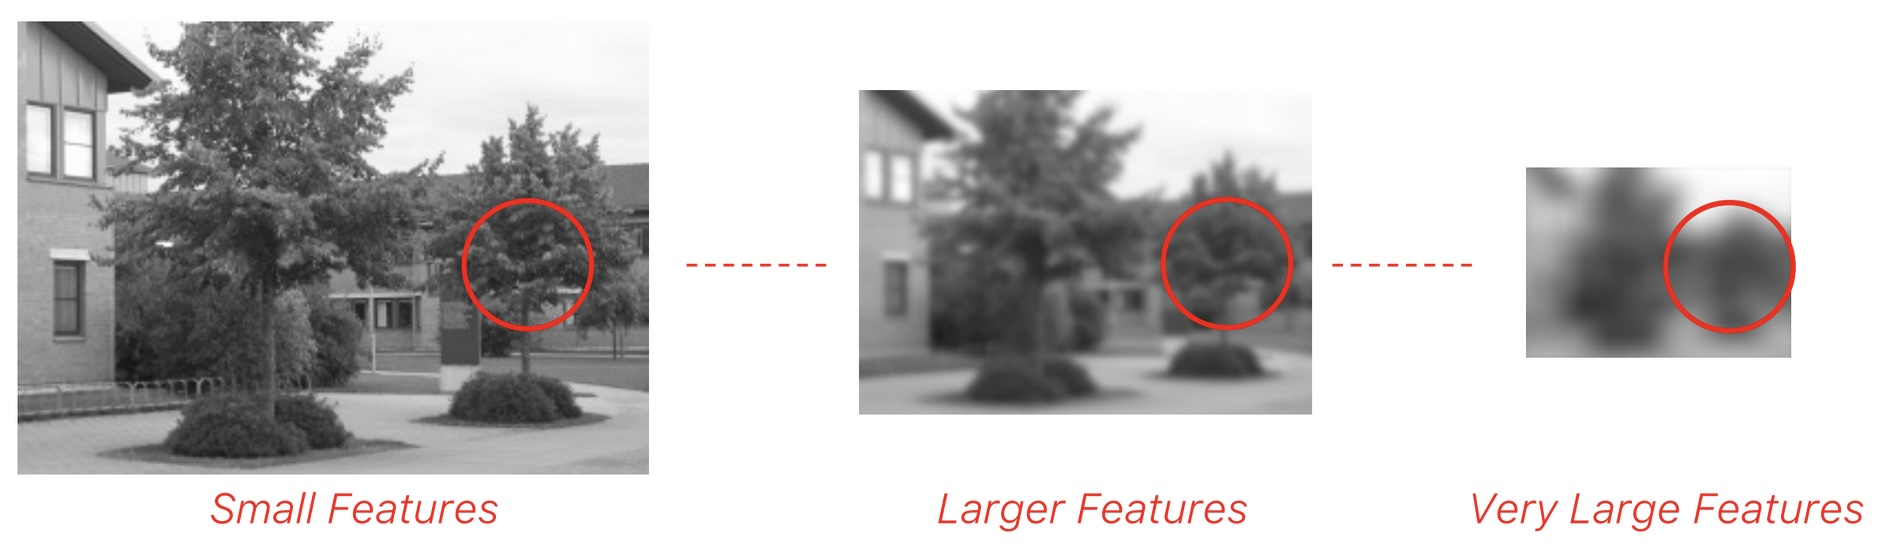
\includegraphics[width=0.9\linewidth]{./img/scale_space.jpg}
  \caption{We increase the blur as we reduce the image size}
  \label{fig:scale_space}
\end{figure}

As we move along scales, small details should continuously disappear and no structure should be introduced.

A Scale-Space is a \textbf{one-parameter family of images} created from the original one so that the structures at smaller scales are successively suppressed by smoothing operations.

A Scale-Space must be realized by Gaussian Smoothing: $L(x,y,\sigma) = G(x,y,\sigma) * I(x,y)$.
A Scale-Space is created by repeatedly smoothing the original image with larger and larger Gaussian kernels.

\paragraph{Feature Detection \& Scale Selection}
% The Gaussian Scale-Space is only a tool to represent the input image at different scales.
% It neither inclues any criterion to detect features nor to select their characteristic scale.
As features exist across a range of scales how do we establish at which scale a feature turns out maximally interesting and should therefore be described?

% The fundamental research work on multi-scale feature detection and automatic scale selection was proposed in "Feature detection with automatic scale selection" by T. Lidneberg in 1998.

As we filter more by using a higher sigma, derivatives tends to become weaker.
To compensate, Lindeberg proposed to multiply/normalize derivatives by sigma (doing scale-normalization).

\paragraph{Scale-Normalized LoG}

The scale-normalized Laplacian Of Gaussian (LoG) is: 
$$F(x,y,\sigma) = \sigma^2\nabla^2 L(x,y,\sigma) = \sigma^2(\nabla^2 G(x,y,\sigma) * I(x,y))$$ where $\sigma^2$ is the normalization factor.

The \textbf{scale-normalized LoG detects blobs} (regions with intensity variations) by combining Gaussian Smoothing (which reduces noise and suppresses fine details) and Laplacian Operator (which highlights regions of rapid intensity change).

Scale normalization is introduced since the raw LoG response diminishes as the scale ($\sigma$) increases, biasing detection toward smaller blobs.

\begin{figure}[htbp]
  \centering
  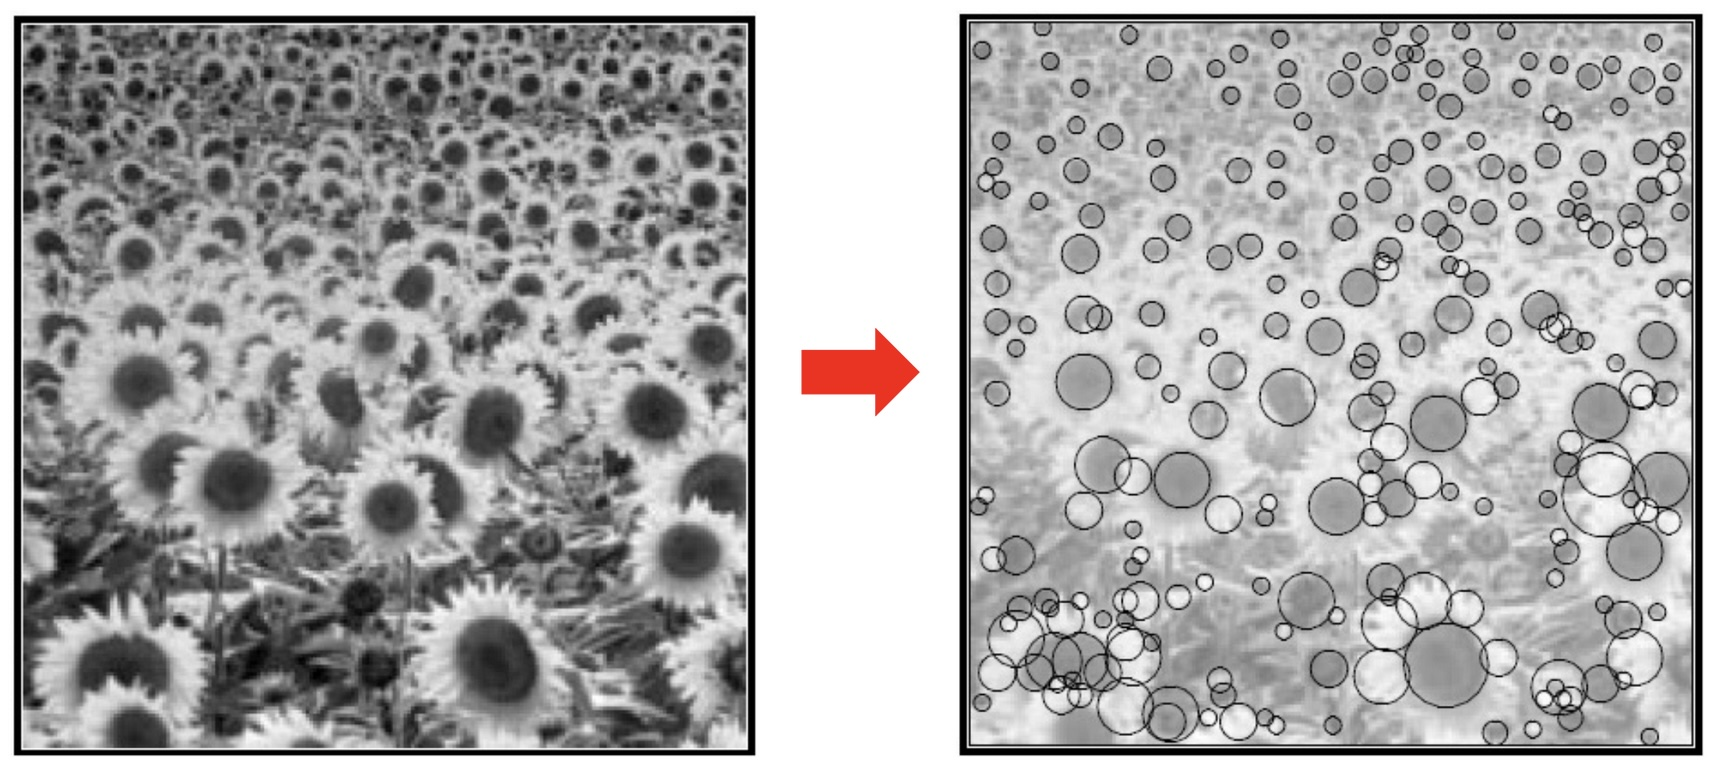
\includegraphics[width=0.7\linewidth]{./img/sunflower_blobs.jpg}
  \caption{LoG filter locates blobs}
  \label{fig:sunflower_blobs}
\end{figure}

\paragraph{Difference of Gaussian (DoG)}

Lowe proposed to detect keypoints by seeking for the extrema of the DoG (Difference of Gaussian) function across the $(x,y,\sigma)$ domain.

$$DoG(x,y,\sigma) = (G(x,y,k\sigma) - G(x,y,\sigma)) * I(x,y) = L(x,y,k\sigma) - L(x,y,\sigma)$$

This approach provides a computationally efficient approximation of Lindeberg's scale-normalized LoG.

$$G(x,y,k\sigma) - G(x,y,\sigma) \approx (k-1)\sigma^2\nabla^2 G(x,y,\sigma) * I(x,y)$$

Both detectors are rotation invariant and find blob-like features.

\begin{figure}[htbp]
  \centering
  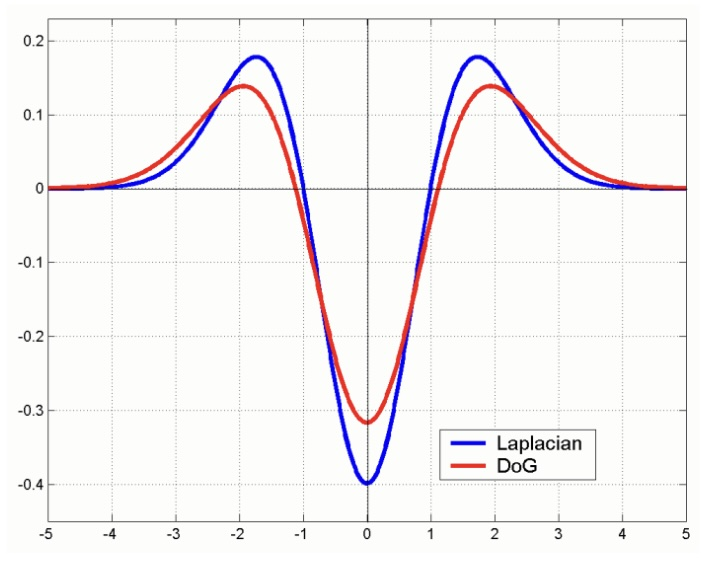
\includegraphics[width=0.5\linewidth]{./img/dog.jpg}
  \caption{Lowe proves that this is a scaled version of Lindeberg}
  \label{fig:dog}
\end{figure}

In the DoG we compute several Gaussian smoothed functions within an octave.
For each pair we take the differences, then we seek for extrema in the DoG.

\begin{figure}[htbp]
  \centering
  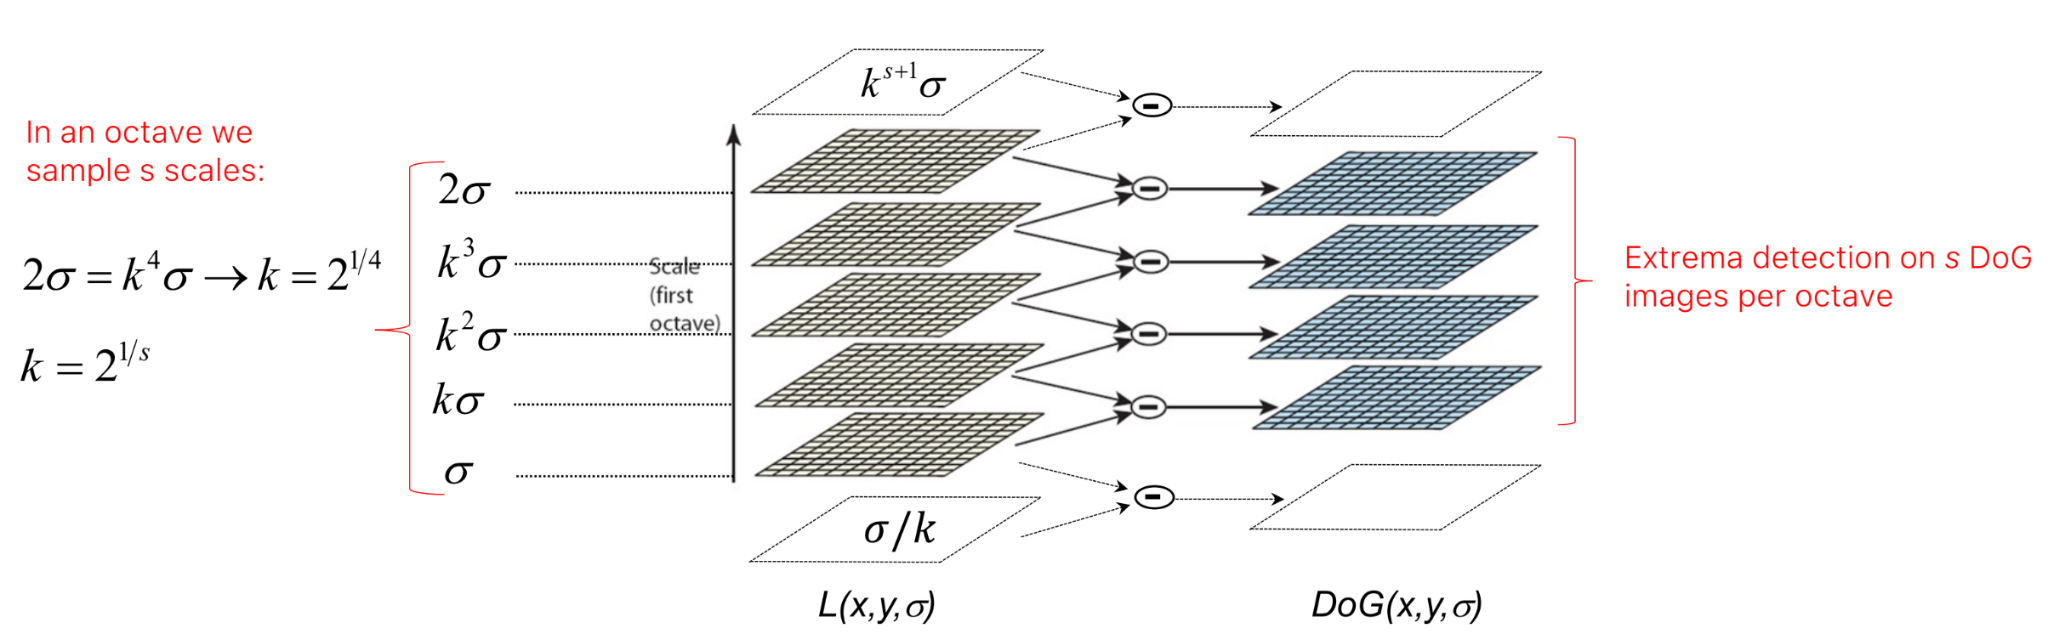
\includegraphics[width=0.9\linewidth]{./img/dog_1.png}
  \caption{Difference of Gaussian}
  \label{fig:dog_1}
\end{figure}

\paragraph{Extrema detection}
A point $(x,y,\sigma)$ is detected as a keypoint if and only if its DoG is higher (or lower) than that of the 26 neighbour (8 at the same scale and $18 =  9 + 9$ at the two nearby scales) in the $(x,y,\sigma)$ space.

According to the original article the best number of sclaes within an octave is $s=3$, initial $\sigma$ for each octave should be $\sigma =1.6$ and the input image is enlarged by a factor of 2 in both dimensions.

After detecting points as local extrema, the next step is to prune weak and unstable responses to ensure robustness.
Keypoints with low contrast, corresponding to weak DoG responses, are often sensitive to noise and less repeatable across different images.

\begin{figure}[htbp]
  \centering
  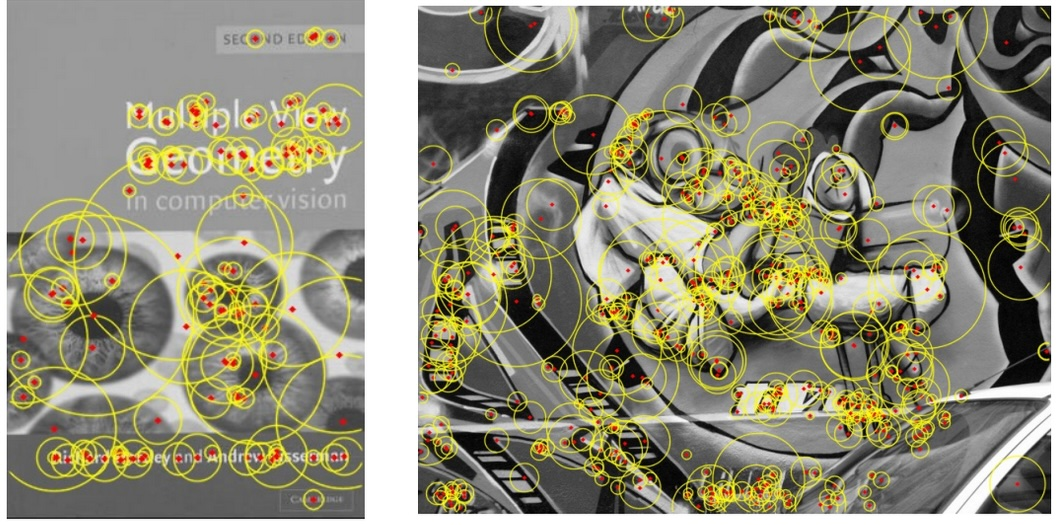
\includegraphics[width=0.7\linewidth]{./img/dog_keypoints.jpg}
  \caption{The size of the circle is proportional to the scale of the feature ($\sigma$)}
  \label{fig:dog_keypoints}
\end{figure}

\subsubsection{Scale and Rotation Invariance Description}

DoG are \textbf{rotation invariant because of circular simmetry}.
Once each keypoint has been extracted, a surrounding patch is considered to compute its descriptor (scale and rotation invariant).

We need to identify a \textbf{prominent direction} inherent to the patch (the canonical orientation) and, based on such direction, define a local reference frame.
A reasonable choice consists in identifying the \textbf{direction along which most of the gradient is found}.

To compute the canoncial orientation we need to define a scale and rotation invariant description.
Once each keypoint has been extracted, a surrounding patch is considered to compute its descriptor (scale and rotation invariant).
\begin{itemize}
  \item Scale invariance: the patch is taken from the stack of images that correspond to the characteristic scale.
  \item Rotation invariance: a canonical patch orientation is computed, so that the descriptor can then be computed on a canonically-oriented patch (orientation with respect to a new reference system, not the one of the image).
\end{itemize}

Lowe proposed to compute the \textbf{canoncial orientation of DoG keypoints} as follows: given the keypoint, the magnitude and orientation of the gradient are computed at each pixel of the associated Gaussian-smoothed image, L:

\begin{itemize}
  \item $m(x,y) = \sqrt{(L(x+1,y)-L(x-1,y))^2 + (L(x,y+1) - L(x,y-1))^2}$
  \item $\theta(x,y) = \tan^{-1}\frac{L(x,y+1)-L(x,y-1)}{L(x+1,y)-L(x-1,y)}$
\end{itemize}

We can then compute an \textbf{orientation histogram} by accumulating the contributions of the pixels belongigng to a neighborhood of the keypoint location (a bin size of $10\deg$).
The characteristic orientation of the keypoint is given by the highest peak of the orientation histogram.
Other peaks higher than $80\%$ of the main one would be kept as well.
A keypoint may have multiple canonical orientations and, in turn, multiple descriptors sharing the same location/scale with diverse orientations (this happen rarely, about on 15\% of the keypoints).

\begin{figure}[htbp]
  \centering
  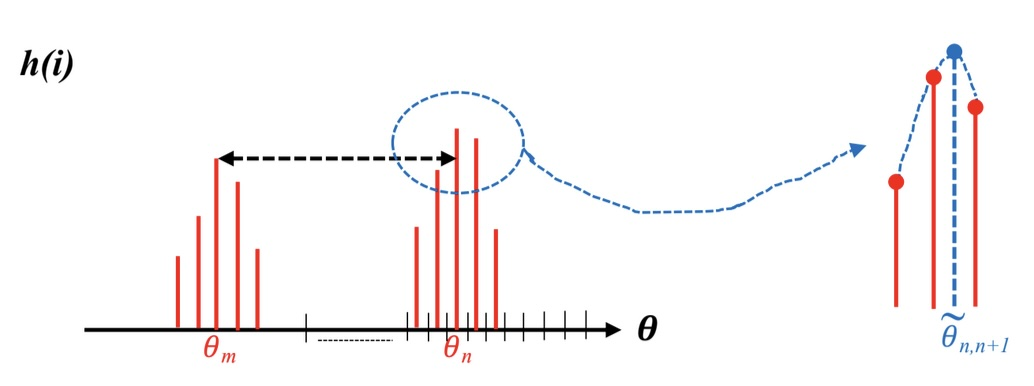
\includegraphics[width=0.7\linewidth]{./img/ambiguous_keypoint.jpg}
  \caption{This is an ambiguous keypoint, we have two prominent decisions}
  \label{fig:ambiguous_keypoints}
\end{figure}

\subsubsection{SIFT Descriptor}

The \textbf{SIFT (Scale Invariant Feature Transform)} descriptor is computed as follows:
\begin{itemize}
  \item $16\times 16$ oriented pixel grid around each keypoint is considered.
  \item This is further divided into $4 \times 4$ regions (each of size $4\times4$ pixels).
  \item A gradient orientation histogram is created for each region.
  \item Each histogram has 8 bins.
  \item Each pixel in the region contributes to its designated bin according to gradient magnitude and gaussian weighting function centered at the keypoint (with $\sigma$ equal to half the grid size).
\end{itemize}

\begin{figure}[htbp]
  \centering
  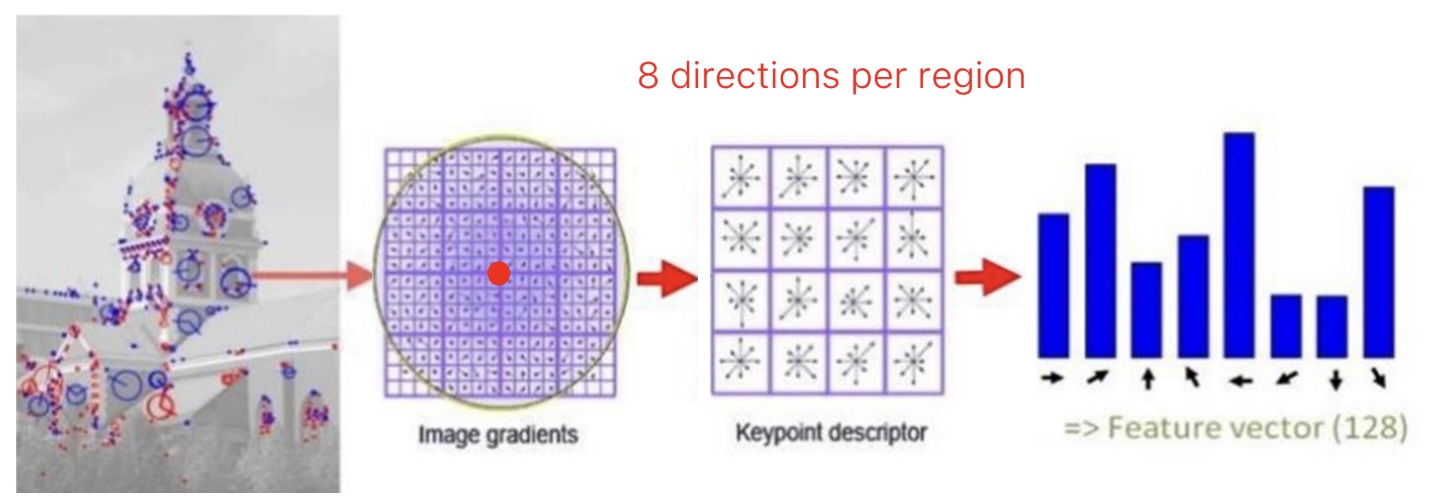
\includegraphics[width=0.8\linewidth]{./img/sift_descriptor.jpg}
  \caption{The descriptor size is given by the number of regions times the number of histogram bins per region}
  \label{fig:sift_descriptor}
\end{figure}

\paragraph{Matching process}
The descriptor is normalized to unit length to gain invariance with respect to affine intensity changes.
Descriptors like SIFT are compared across diverse views of a scene to find corresponding keypoints.
This is a classical Nearest Neighbour (NN) seach problem.
Given a set $S$ of points, $p_i$, in a matric space $M$ and a query point $q \in M$, find the $p$, closest to $q$.
We wish to match the local features computed from an image under analysis (target image $T$) to those already computed from a reference image ($R$) or a set of reference images.

For each feature in $T$ we look for the most similar one in $R$:
\begin{itemize}
  \item The features in $T$ represent the query points, $q$.
  \item The features in $R$ provide set $S$.
  \item When matching SIFT descriptors the distance typically used is the Euclidean distance.
\end{itemize}

\begin{figure}[htbp]
  \centering
  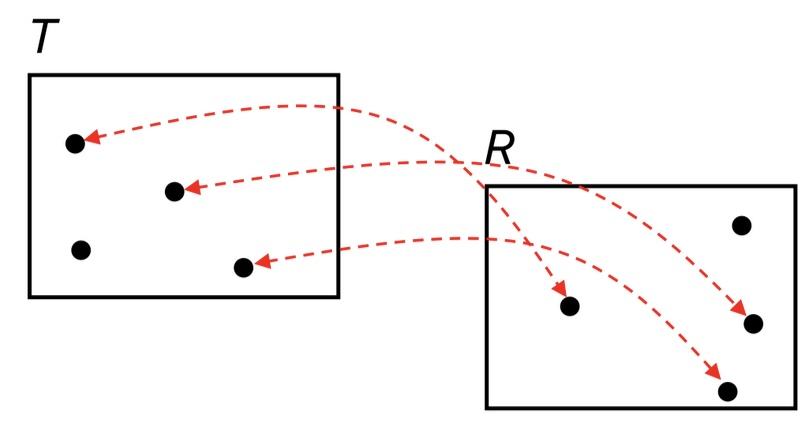
\includegraphics[width=0.5\linewidth]{./img/matching_sift.jpg}
  \caption{Image matching process with SIFT}
  \label{fig:matching_sift}
\end{figure}

The found Nearest Neighbour (NN) does not necessarily provide a valid correspondence as some features in $T$ may not have a corresponding feature in $R$.
We enforce a criteria to accept/reject a match found by the NN search process.
The simplest thing to do is to use a threshold.
Lowe showed that $T=0.8$ may allow for rejecting $90\%$ of the wrong matches while missing only $5\%$ of those correct.

Exhaustively searching for the NN of the query feature, $q$, has linear complexity in the size of $S$.
This is slow, so efficient indexing techniques are exploited to speed-up the NN-search process.
The main indexing technique exploited for feature matching is known as k-d tree.

% ==============================================================================

% \subsection{Camera Calibration}

% Camera Calibration is important for taking quantitative measurements from images.
% In the \textbf{perspective projection} model, given a point in the 3D space $M = [x,y,z]^T$, with coordinates given in the Camera Reference Frame (CRF).
% Its projection onto the image plane I is denoted as $m=[u,v]^T$.

% \begin{figure}[htbp]
%   \centering
%   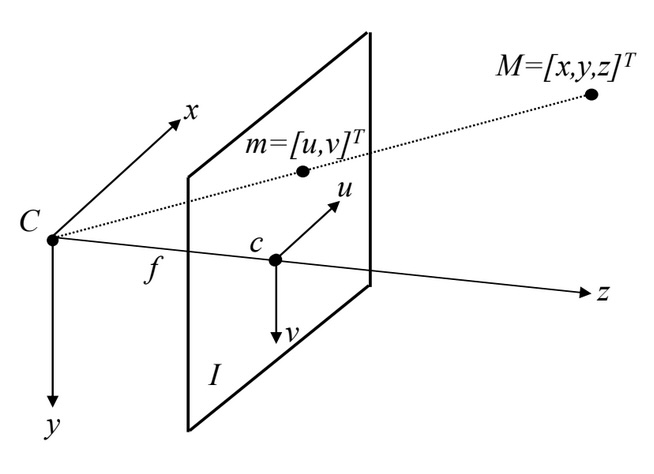
\includegraphics[width=0.5\linewidth]{./img/camera_calibration.jpg}
%   \caption{Perspective Projection Model (PPM)}
%   \label{fig:camera calibration}
% \end{figure}

% \subsubsection{Projective Space}

% The \textbf{Physical Space} is a 3D Euclidean Space ($\mathbb{R}^3$) whose points can be represented as 3D vectors in a given reference frame.
% In this space parallel lines do not intersect.
% Points at infinity cannot be represented in this vector space.

% The \textbf{Projective Space} is a mathematical engine to handle the geometry of image formations.
% In the Projective space we append one more coordinate to the Euclidean triplets.
% A point is represented by an equivalence class of quadruples, wherein equivalent quadruples differ just by a multiplicative factor.
% This is called the \textbf{homogeneous coordinates} representation of the 3D point having Euclidean coordinates $(x,y,z)$.
% The space associated with the homogeneous coordinate's representation is called Projective Space, denoted as $P^3$

% \vspace{0.6em}
% We are interested in Projective Spaces because Perspective Projection is \textbf{more conveniently} dealt with using projective coordinates.
% \vspace{0.6em}

% The point at infinity is a point in the space, the vanishing point is a point into the image plane.
% Points at infinity of the 3D lines are the points of the 3D Projective Space \textbf{having the fourth coordinate equal to 0}.

% To map such points into the Euclidean Space we would divide by the fourth coordinate (which is 0) which is not a valid representation in the Euclidean Space.

% The point $(0,0,0,0)$ it's not the origin, but an undefined point. The origin is represented in homogeneous coordinates as $(0,0,0,k)$, with $k\neq 0$.

% Given a 3D point $\tilde{M} = [x,y,z]^T$ (with coordinates expressed in the Camera Reference Frame) and its 2D projection onto the image plane $\tilde{m} = [u,v]^T$.

% In homogeneous coordinates the perspective projection becomes a linear transformation.

% $$
% \begin{bmatrix}
% u \\ v \\ 1
% \end{bmatrix} =
% \begin{bmatrix}
% f & 0 & 0 & 0 \\
% 0 & f & 0 & 0 \\
% 0 & 0 & 1 & 0 
% \end{bmatrix}
% \begin{bmatrix}
% x \\ y \\ z \\ 1
% \end{bmatrix}
% $$

% Which in matrix notation is $\tilde{m} \approx \tilde{P}\tilde{M}$, where $\approx$ means "equal up to an arbitrary scale factor".
% \vspace{1em}
% $\tilde{P}$ represents the geometric camera model, and is known as \textbf{Perspective Projection Matrix (PPM)}.

% \vspace{1em}

% The operation carried out by the PPM is that of scaling lateral coordinates according to the distance from the camera $(z)$.
% The actual focal length just introduces an additional scaling factor of projected coordinates.

% \subsubsection{A more comprehensive camera model}

% To create a more realistic camera model we need to consider three additional issues:
% \begin{enumerate}
%   \item Image coordinates are usually expresed in an image reference frame with the origin in the top left corner.
%   \item Images are a grid of pixels, not a continuous plane (pixelization).  The digitization can be accounted for by including into the projection equations the pixel size $\Delta u$ and $\Delta v$ along the two axes (typically they have the same value).
%   \item We do not normally know or want to project back the coordinate of a 3D point in the Camera Reference Frame, but in some generic World Reference Frame, that we place where it's most comfortable for us.
% \end{enumerate}

% \paragraph{Intrinsic Parameter Matrix}

% The matrix $A$, models the intrinsic characteristics (Intrinsic Parameters) of the image sensing device (focal length, pixel dimension...) and is called \textbf{Intrinstic Parameter Matrix}
% The smallest number of intrinsic parameters is thus 4 ($f_u, f_v$ and the coordinates of the piercing point $c(u_0, v_0)$).
% They represent the camera geometry, which is independent of its position in the world.

% Now the Perspective Projection Matrix can be written as:
% $$
% \tilde{P} = 
% \begin{bmatrix}
%   fk_u & 0 & u_0 & 0 \\
%   0 & fk_v & v_0 & 0 \\
%   0 & 0 & 1 & 0 
% \end{bmatrix}
% =
% \begin{bmatrix}
%   fk_u & 0 & u_0 \\
%   0 & fk_v & v_0 \\
%   0 & 0 & 1 
% \end{bmatrix}
% \begin{bmatrix}
%   1 & 0 & 0 & 0 \\
%   0 & 1 & 0 & 0 \\
%   0 & 0 & 1 & 0 
% \end{bmatrix}
% = A[I|0]
% $$

% We can now see that if we have $[a,b,c,0]$, which are the coordinates of a point in the WRF. By using the Perspective Projection matrix we can do this calculation:

% $$
% \tilde{m}_{\infty} =
% P_{int}
% \begin{bmatrix}
% a \\ b \\ c \\ 0
% \end{bmatrix}
% =
% \begin{bmatrix}
%   fk_u & 0 & u_0 & 0 \\
%   0 & fk_v & v_0 & 0 \\
%   0 & 0 & 1 & 0 
% \end{bmatrix}
% \begin{bmatrix}
% a \\ b \\ c \\ 0
% \end{bmatrix}
% =
% \begin{bmatrix}
% f_u a + c u_0 \\
% f_v b + c v_0 \\
% c
% \end{bmatrix}
% $$

% The final vector can be divided by $c$ (the third component) and we get the coordinates of the point at infinity in an image: $m_{\infty} = \begin{bmatrix} f_u \frac{a}{c} + u_0 \\ f_v \frac{b}{c} + v_0\end{bmatrix}$.

% This handles all the cases except $c = 0$, which is the case of a line parallel to the camera sensor.

% \paragraph{Rigid motion between CRF and WRF}
% We need to apply a roto-translation to relate the World Reference Frame to the Camera Reference Frame.
% The relation between the coordinates of a point in the two reference frames is:

% $$
% W =
% \begin{bmatrix}
% X \\ Y \\ Z \\ 1
% \end{bmatrix}
% \,,
% M=
% \begin{bmatrix}
% x\\ y\\ z\\1
% \end{bmatrix}
% \Rightarrow
% M=
% \begin{bmatrix}
% R & T \\
% 0 & 1
% \end{bmatrix}
% W = GW
% $$

% To map a 3D point expressed in the Camera Reference Frame: $k\tilde{m} = A[I|0]\tilde{M}$

% The general from of the Perspective Projection Matrix can be expressed as follows:
% $\tilde{P} = A[I|0]G$ or also $\tilde{P}=A[R|T]$.

% \paragraph{Extrinsic Parameters}

% $G$ is called \textbf{Extrinsic Parameter Matrix} and it encodes the position and orientation of the camera with respect to the World Reference Frame.
% The rotation matrix has only 3 independent parameters, which correspond to the rotation angles around the axis of the reference frame.
% $T$ has 3 independent parameters.
% The total number of \textbf{extrinsic parameters} is 6 (3 translation, 3 rotation).
% $A$ has 4 independent parameters.
% The general form of the Perspective Projection Matrix can be thought of as encoding:
% \begin{itemize}
%   \item the position of the camera with respect to the world into $G$.
%   \item the actual characteristics of the sensing device into $A$.
% \end{itemize}

% ==============================================================================

\subsection{Camera Calibration}

Camera calibration is the process of determining the parameters of a camera model that describes how a 3D scene is projected onto a 2D image. This is crucial for extracting quantitative measurements from images, such as object sizes or distances. We primarily focus on the \textbf{perspective projection} model.

\begin{figure}[htbp]
  \centering
  % Make sure the image path is correct relative to your main LaTeX file
  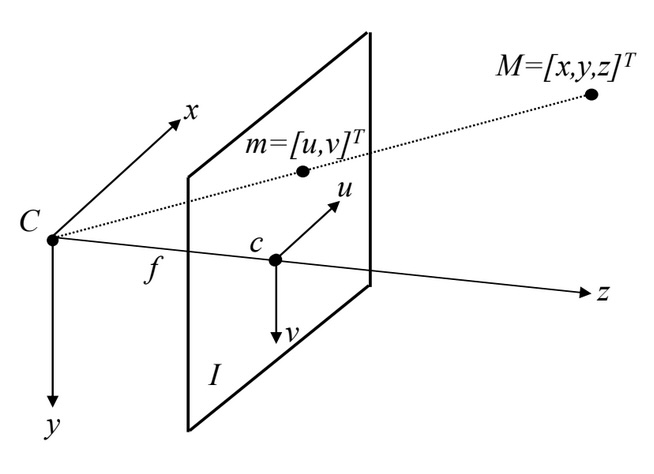
\includegraphics[width=0.5\linewidth]{./img/camera_calibration.jpg}
  \caption{Perspective Projection Model (PPM). A 3D point $M$ in the Camera Reference Frame (CRF) projects to a 2D point $m$ on the image plane $I$.}
\end{figure}

\subsubsection{From Physical Space to Projective Space}

The world we perceive is often modeled as a 3D \textbf{Euclidean Space} ($\mathbb{R}^3$). Points are represented by 3D vectors $[x, y, z]^T$ in a chosen reference frame. However, Euclidean geometry struggles with concepts like points at infinity and the projective nature of image formation (e.g., parallel lines appearing to converge).

To handle the geometry of perspective projection more elegantly, we use \textbf{Projective Space} ($P^3$).
\begin{itemize}
    \item \textbf{Homogeneous Coordinates:} A point with Euclidean coordinates $(x, y, z)$ is represented in homogeneous coordinates by an equivalence class of 4D vectors $[\lambda x, \lambda y, \lambda z, \lambda]^T$ for any non-zero scalar $\lambda$. A common choice is to set $\lambda=1$, giving $[x, y, z, 1]^T$.
    \item \textbf{Mapping Back:} To convert from homogeneous coordinates $[X, Y, Z, W]^T$ (where $W \neq 0$) back to Euclidean coordinates, we divide by the fourth component: $[X/W, Y/W, Z/W]^T$.
    \item \textbf{Points at Infinity:} Points at infinity correspond to directions in 3D space. In homogeneous coordinates, they are represented by vectors of the form $[X, Y, Z, 0]^T$, where $[X, Y, Z]^T$ defines the direction. These points cannot be mapped back to the finite Euclidean space.
    \item \textbf{The Origin:} The origin of the Euclidean space $(0,0,0)$ is represented by $[0, 0, 0, k]^T$ with $k \neq 0$ in homogeneous coordinates. The vector $[0, 0, 0, 0]^T$ is undefined in projective space.
\end{itemize}
The main advantage of using homogeneous coordinates is that the non-linear perspective projection equations become \textbf{linear transformations} represented by matrix multiplication.

\subsubsection{Basic Perspective Projection Matrix (Pinhole Camera)}

Let $M = [x, y, z]^T$ be a 3D point expressed in the \textbf{Camera Reference Frame (CRF)}, with the origin at the camera's optical center and the z-axis along the optical axis. Let its projection onto the image plane be $m = [u, v]^T$. Assuming the image plane is at $z=f$ (where $f$ is the focal length), the basic perspective projection is:
$u = f \frac{x}{z}$ and $v = f \frac{y}{z}$.

Using homogeneous coordinates, we represent the 3D point as $\tilde{M}_{CRF} = [x, y, z, 1]^T$ and the projected 2D point as $\tilde{m} = [u', v', w']^T$, where the final image coordinates are $u = u'/w'$ and $v = v'/w'$. The projection can be written as a linear mapping:

% Using \propto or \approx clarifies equality up to scale
%tilde{m} = [u', v', w']^T = [fx, fy, z]^T
% The matrix maps [x,y,z,1] to [fx, fy, z]. To get the final homogeneous image point [u,v,1], we need a slightly different matrix.
% The matrix below maps [x,y,z,1] to [fx, fy, z, z] in P^3, but image points are in P^2.
% Let's use the common 3x4 projection matrix directly mapping 3D homogeneous points to 2D homogeneous points.
\[
w' % Scaling factor, which turns out to be z
\begin{bmatrix}
u \\ v \\ 1
\end{bmatrix}
=
\begin{bmatrix}
f & 0 & 0 & 0 \\
0 & f & 0 & 0 \\
0 & 0 & 1 & 0
\end{bmatrix}
\begin{bmatrix}
x \\ y \\ z \\ 1
\end{bmatrix}
\]
This can be written compactly as $\tilde{m} \propto P_0 \tilde{M}_{CRF}$, where $\propto$ denotes equality up to a non-zero scale factor, and $P_0$ is the basic $3 \times 4$ perspective projection matrix for a pinhole camera centered at the origin, looking along the z-axis. The scale factor here is $w'=z$.

% Note: The original text had a 4x4 matrix, which is less standard for mapping 3D points to 2D image points.
% The 3x4 matrix formulation is more common as it directly produces the 3-vector homogeneous image coordinates.

\subsubsection{A More Comprehensive Camera Model}

The basic model is often insufficient. We need to account for:
\begin{enumerate}
  \item \textbf{Image Coordinate System:} Image coordinates $(u, v)$ are typically measured in pixels, with the origin often at the top-left corner, not the principal point (where the optical axis pierces the image plane).
  \item \textbf{Pixel Shape:} Pixels might not be square. We need parameters for pixel size/density $(\Delta u, \Delta v)$ or equivalently, focal lengths measured in pixels ($f_u = f/\Delta u$, $f_v = f/\Delta v$).
  \item \textbf{World Reference Frame (WRF):} 3D points are usually defined in a convenient WRF, not the CRF. We need to relate the WRF to the CRF.
\end{enumerate}

These factors lead to a more complex projection matrix $\tilde{P}$, which can be decomposed into intrinsic and extrinsic parameters.

\paragraph{Intrinsic Parameter Matrix (A)}
This $3 \times 3$ matrix maps projected points from the camera's normalized image plane (where $z=1$) to pixel coordinates. It encodes the camera's internal geometry:
\begin{itemize}
    \item $f_u, f_v$: Focal lengths expressed in units of horizontal and vertical pixel dimensions.
    \item $(u_0, v_0)$: Coordinates of the principal point (the image center) in pixels. Sometimes denoted $(c_x, c_y)$.
    % Optional: Skew parameter 's' can be added if axes are not perfectly orthogonal, though often assumed zero.
    % \item s: Skew coefficient between the x and y axis (often 0).
\end{itemize}
Assuming zero skew, the intrinsic matrix is:
\[
A =
\begin{bmatrix}
  f_u & 0 & u_0 \\
  0 & f_v & v_0 \\
  0 & 0 & 1
\end{bmatrix}
\]
These \textbf{intrinsic parameters} (at least 4: $f_u, f_v, u_0, v_0$) are specific to the camera and lens, independent of the camera's position or orientation in the world.

The projection from the CRF using only intrinsic parameters can be written by combining $A$ with a standard projection into the normalized image plane:
\[
\tilde{P}_{int} = A [I | \mathbf{0}] =
\begin{bmatrix}
  f_u & 0 & u_0 & 0 \\
  0 & f_v & v_0 & 0 \\
  0 & 0 & 1 & 0
\end{bmatrix}
\]
This matrix $\tilde{P}_{int}$ maps a 3D point in homogeneous coordinates \emph{relative to the CRF} to its 2D homogeneous pixel coordinates.

% The calculation for vanishing points can be illustrated here, as in the original text.
% It shows how directions (points at infinity) relative to the camera project into the image.
\paragraph{Vanishing Points Example}
Consider a point at infinity $[a, b, c, 0]^T$ representing a direction relative to the CRF. Its projection using $\tilde{P}_{int}$ is:
\[
\tilde{m}_{\infty} \propto \tilde{P}_{int}
\begin{bmatrix} a \\ b \\ c \\ 0 \end{bmatrix}
=
\begin{bmatrix}
  f_u a + u_0 c \\
  f_v b + v_0 c \\
  c
\end{bmatrix}
\]
Assuming $c \neq 0$ (the direction is not parallel to the image plane), we can convert to Euclidean pixel coordinates by dividing by the third component:
\[
m_{\infty} = \begin{bmatrix} f_u \frac{a}{c} + u_0 \\ f_v \frac{b}{c} + v_0 \end{bmatrix}
\]
This projected point $m_{\infty}$ is a \textbf{vanishing point} in the image – the point where parallel lines in 3D space with direction $[a, b, c]^T$ appear to converge. If $c=0$, the direction is parallel to the image plane, and the point projects to infinity in the image plane coordinates (no finite vanishing point).


\paragraph{Extrinsic Parameter Matrix (G)}
To use points defined in a World Reference Frame (WRF), we need to describe the camera's pose (position and orientation) relative to the WRF. This is done using a rigid body transformation:
\begin{itemize}
    \item $R$: A $3 \times 3$ rotation matrix describing the orientation of the CRF relative to the WRF.
    \item $T$: A $3 \times 1$ translation vector describing the position of the CRF origin relative to the WRF origin (expressed in WRF coordinates). Or sometimes, the position of the WRF origin relative to the CRF origin (expressed in CRF coordinates) - convention matters! Let's assume $T$ specifies the CRF origin in WRF for the $G$ matrix below which transforms points *from* WRF *to* CRF.
\end{itemize}
The transformation from WRF coordinates $\tilde{M}_W = [X, Y, Z, 1]^T$ to CRF coordinates $\tilde{M}_{CRF} = [x, y, z, 1]^T$ is given by:
\[
\tilde{M}_{CRF} = G \tilde{M}_W
\]
where $G$ is the $4 \times 4$ \textbf{Extrinsic Parameter Matrix}. A common form relates WRF coordinates to CRF coordinates:
\[
% This form transforms points FROM World TO Camera Frame
% M_CRF = [R | -RC_W] M_W   where C_W is camera center in World coords
% OR M_CRF = [R | T_crf] M_W where T_crf is WRF origin in CRF coords.
% Let's use the [R|T] notation where T is the translation part defining the camera frame coords from world coords.
% Standard notation often uses T = -RC_w where C_w is the world coordinate of the camera center.
% The original notes wrote M = G W where M is CRF and W is WRF.
% M = [R T; 0 1] W means x_crf = R X_w + T. This T is the WRF origin expressed in CRF coords.
G = \begin{bmatrix} R & T \\ \mathbf{0}^T & 1 \end{bmatrix}
\]
Here, $R$ rotates the WRF axes to align with the CRF axes, and $T$ translates the origin. This transformation has \textbf{6 extrinsic parameters}: 3 for rotation (e.g., Euler angles, axis-angle) and 3 for translation.

% Note: The definition G = [R T; 0 1] means T is the vector from the WRF origin to the CRF origin, expressed in CRF coordinates.
% Alternatively, if G transforms world to camera, it's often written as G = [R | -RC_w], where C_w is camera center in world coordinates. The final [R|T] in P = A[R|T] uses T = -RC_w. Let's adjust to match the standard P = A[R|T] formulation.

The transformation from WRF to CRF coordinates (non-homogeneous) is $M_{crf} = R M_w + T'$, where $T'$ is the translation vector. In homogeneous coordinates, this is often expressed using a $4\times4$ matrix that incorporates the inverse transformation or directly within the projection matrix.

\subsubsection{The Complete Perspective Projection Matrix (\~{P})}

Combining the intrinsic and extrinsic parameters, the full projection from a 3D point $\tilde{M}_W$ in WRF homogeneous coordinates to a 2D point $\tilde{m}$ in image homogeneous pixel coordinates is:
\[
\tilde{m} \propto A [R | T] \tilde{M}_W
\]
Here, the $3 \times 4$ matrix $\tilde{P} = A[R|T]$ is the complete \textbf{Perspective Projection Matrix (PPM)}.
\begin{itemize}
    \item $R$ is the $3 \times 3$ rotation matrix specifying the camera's orientation.
    \item $T$ is the $3 \times 1$ translation vector specifying the camera's position (specifically, $T = -RC_W$, where $C_W$ is the position of the camera center in world coordinates).
\end{itemize}
The matrix $[R|T]$ effectively transforms the point from WRF coordinates directly into the CRF, ready for projection and intrinsic transformation by $A$.

The PPM $\tilde{P}$ encodes all the geometric information of the camera setup:
\begin{itemize}
    \item Intrinsic parameters ($A$): Camera's internal geometry (focal length, principal point, pixel properties). (4+ parameters)
    \item Extrinsic parameters ($R, T$): Camera's pose (position and orientation) in the world. (6 parameters)
\end{itemize}
Camera calibration aims to find the numerical values for the parameters in $A$ and, often simultaneously or subsequently, the extrinsic parameters $R$ and $T$ relative to a known calibration target.

% 55:06

\subsubsection{P as a Homography}
We just need the relation between the camera and the plane, then we can measure everything on that plane.

If the camera is imaging a planar scene, we can assume the z-axis of the World Reference Frame to be perpendicular to the plane such that all 3D points will have their z-coordinate equal to 0.
The Perspective Projection Matrix then becomes a simpler transformation defined by a $3x3$ matrix.
$$k\tilde{m} = \tilde{P}\tilde{w}
\begin{bmatrix}
  p_{1,1} & p_{1,2} & \cancel{p_{1,3}} & p_{1,4} \\
  p_{2,1} & p_{2,2} & \cancel{p_{2,3}} & p_{2,4} \\
  p_{3,1} & p_{3,2} & \cancel{p_{3,3}} & p_{3,4} 
\end{bmatrix}
\begin{bmatrix}
x \\ y \\ 0 \\ 1
\end{bmatrix}
=
\begin{bmatrix}
  p_{1,1} & p_{1,2} & p_{1,4} \\
  p_{2,1} & p_{2,2} & p_{2,4} \\
  p_{3,1} & p_{3,2} & p_{3,4} 
\end{bmatrix}
\begin{bmatrix}
x \\ y \\ 1
\end{bmatrix}
= H\tilde{M}
$$

Such a transformation, denoted here as H, is known as \textbf{homography} and represents a general linear transformation between projective planes.
A homography is then a projective transformation between two planes or a mapping between two planar projection of an image.

\begin{figure}[htbp]
  \centering
  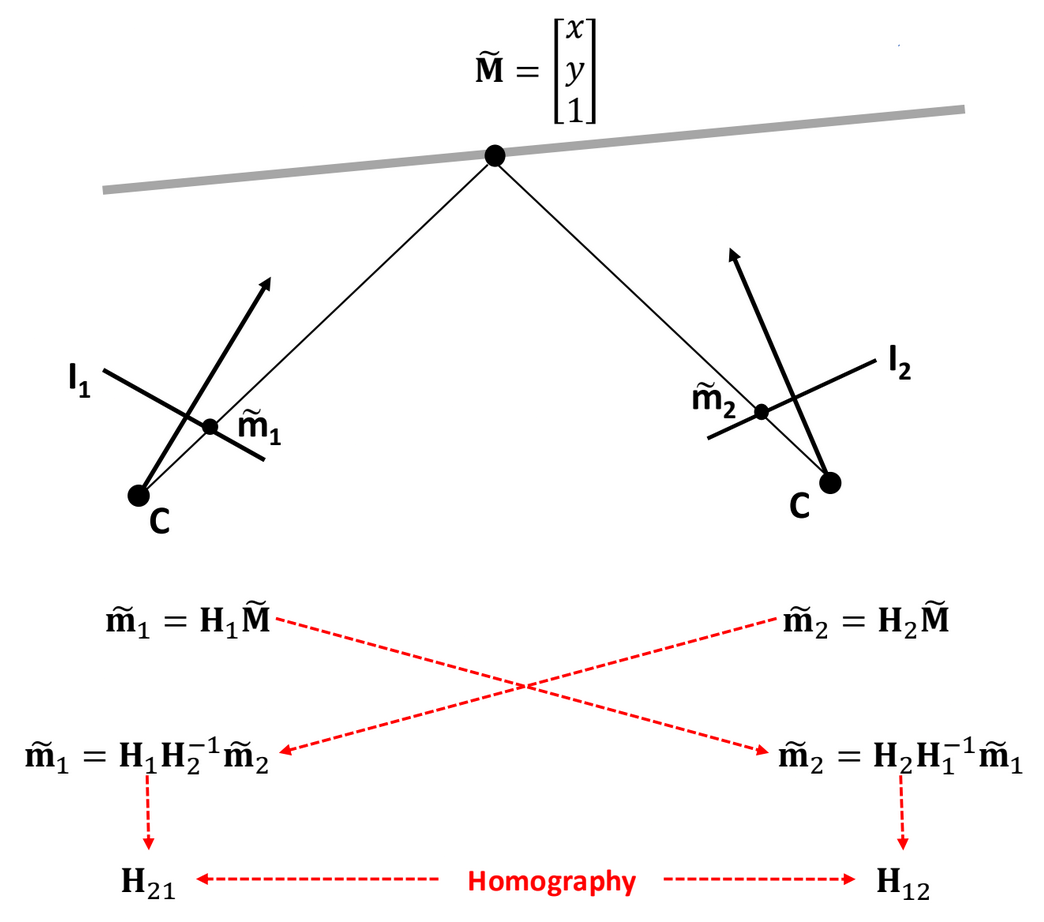
\includegraphics[width=0.6\linewidth]{./img/homography.jpg}
  \caption{Any two images of a planar scene are related by a homography}
  \label{fig:homography}
\end{figure}

\begin{figure}[htbp]
  \centering
  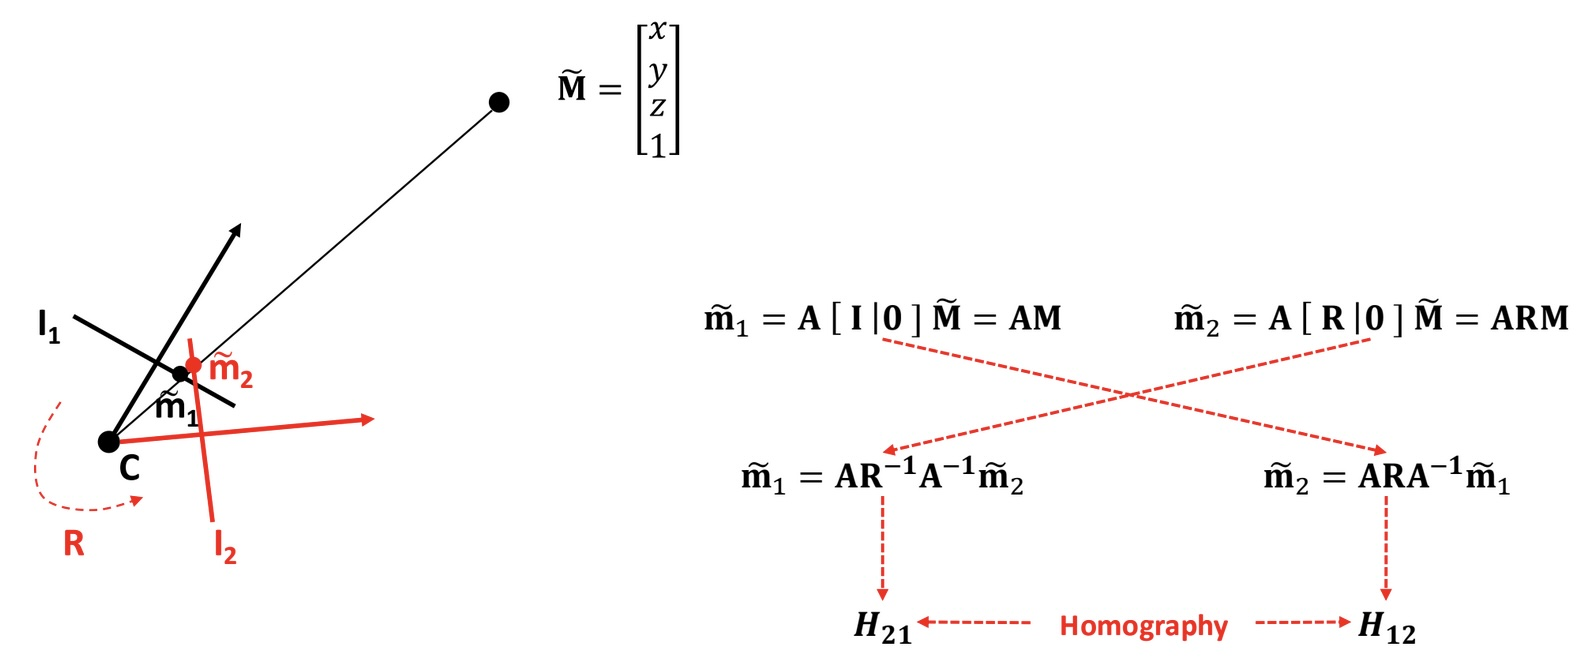
\includegraphics[width=0.8\linewidth]{./img/rotating_homography.jpg}
  \caption{Any two images taken by a camera rotating about the optical center are related by a homography}
  \label{fig:rotating_homography}
\end{figure}

\begin{figure}[htbp]
  \centering
  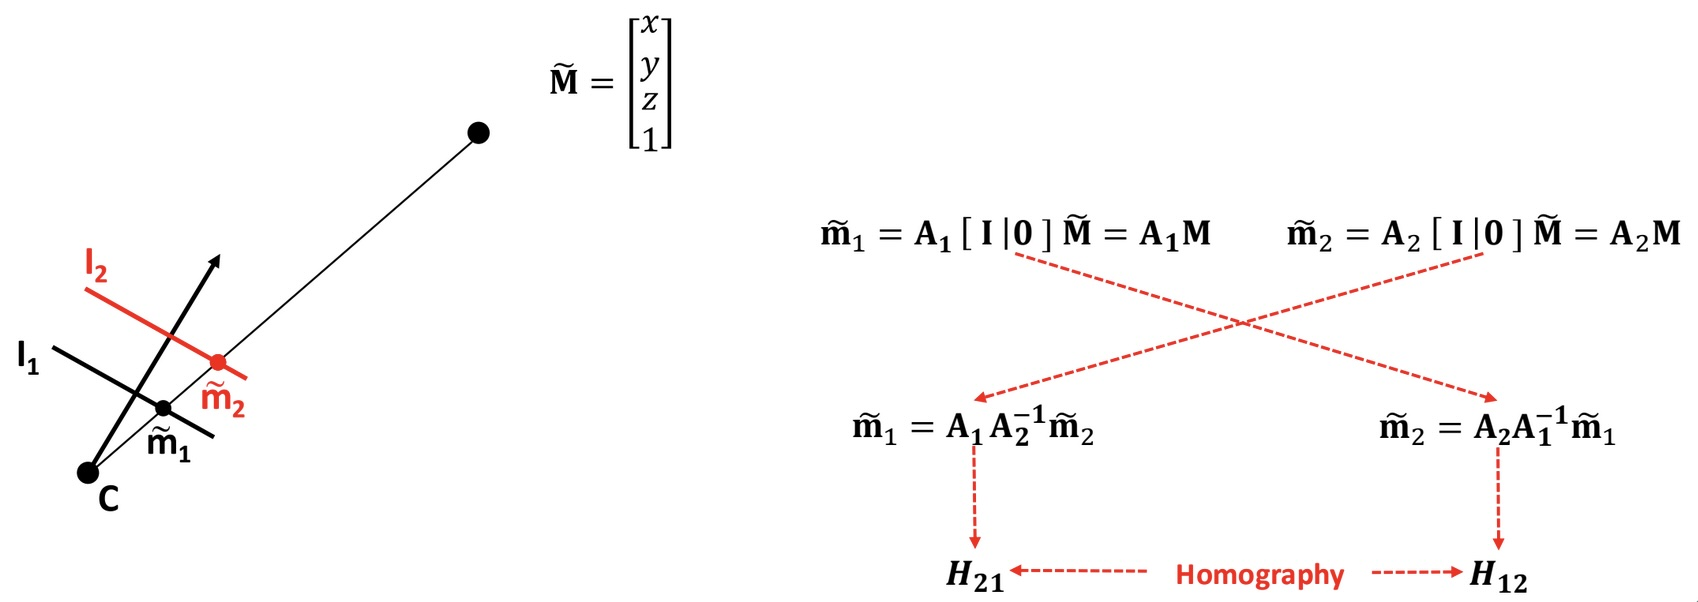
\includegraphics[width=0.8\linewidth]{./img/moving_homography.jpg}
  \caption{Any two images taken by different cameras in fexed pose are related bu a homography}
  \label{fig:moving_homography}
\end{figure}

\subsubsection{Lens distortion}

The Perspective Projection Matrix is based on the pinhole camera model, however, real lenses introduce distortions with respect to the pure pinhole model.
We also have lens distortion, which is modelled through additional parameters that don't alter the form of the Perspective Projection Matrix.

We have two types of lens distortion: barrel distortion which bends straight lines outwards, and pincushion distortion, which causes straight lines to curve inward.

\subsubsection{Calibration}

We now have the Perspective Projection Matrix camera model, which can be decomposed in:
\begin{itemize}
  \item Intrinsic parameter matrix $A$.
  \item Rotation matrix $R$.
  \item Translation vector $T$.
\end{itemize}

\textbf{Camera calibration} is the process where \textbf{all parameters defining the camera model are estimated} for a specific camera device.
Depending on the application, \textbf{either the Perspective Projection Matrix (PMM) only, or also its independent components} ($A$,$R$,$T$) need to be estimated.

There are many camera calibration algorithms, but the basic process always relies on setting up a linear system of equations given a set of known 3D-2D correspondences.
To obtain the correspondences we use calibration targets, which have easily detectable features.

The approaches can be split into:
\begin{itemize}
  \item Those relying on a single image containing a known pattern.
  \item Those relying on several different images of one given planar pattern.
\end{itemize}

Since in every frame we change the relative position of the camera and the pattern, we will have a different set of extrinsic parameter for each image.
We will have just one set of intrinsic parameter since the camera is always the same across the different pictures.

\subsubsection{Zhang's method for Camera Calibration}

We use a chessboard pattern of which we know the number of internal corners and the size of the squares.
Internal corners can be easily detected by standard algorithms, like the Harris corner detector.
Typically the camera is fixed and you move the calibration target in front of the camera.
The $[R\,T]$ are estimated with respect to the reference system attached to the target, but it changes alongside with the pattern.
In each image the 3D world reference frame is taken at the top-left corner of the pattern.
Each image requires its own estimate of the extrinstic parameters, as they are different from one to the other.
Due to the choice of the world reference frame associated with calibration images, in each of them we consider only 3D points with $z=0$.
The Perspective Projection Matrix boils down to a simpler transformation defined by an homography $3\times 3$ matrix, like with $P$ as a homography.

$$k\tilde{m} = \tilde{P}\tilde{w}
\begin{bmatrix}
  p_{1,1} & p_{1,2} & \cancel{p_{1,3}} & p_{1,4} \\
  p_{2,1} & p_{2,2} & \cancel{p_{2,3}} & p_{2,4} \\
  p_{3,1} & p_{3,2} & \cancel{p_{3,3}} & p_{3,4} 
\end{bmatrix}
\begin{bmatrix}
x \\ y \\ \cancel{0} \\ 1
\end{bmatrix}
=
\begin{bmatrix}
  p_{1,1} & p_{1,2} & p_{1,4} \\
  p_{2,1} & p_{2,2} & p_{2,4} \\
  p_{3,1} & p_{3,2} & p_{3,4} 
\end{bmatrix}
\begin{bmatrix}
x \\ y \\ 1
\end{bmatrix}
= H\tilde{M}
$$

\paragraph{Estimating $H_i$ (DLT algorithm)}
Given a pattern with $m$ corners, we can write $m$ systems of 3 linear equations, where:
\begin{itemize}
  \item Both 3D as well as 2D coordinates are known due to the corners having been detected in the i-th image and the unknowns are thus the 9 elements in $H_i$.
  \item $H_i$ (and $P_i$ alike) is known up to an arbitrary scale factor, the independent elements in $H_i$ are 8.
\end{itemize}

\textbf{There are plenty of methods for the estimation}

The Zhang's method can be summarized as:
\begin{enumerate}
  \item Acquire $n$ images of a planar pattern with $m$ internal corners.
  \item For each image compute an initial guess for homography $H_i$.
  \item Refine eaech $H_i$ by minimizing the reprojection error.
  \item Get an initial guess for $A$ given the homographies $H_i$.
  \item Given $A$ and $H_i$, get an initial guess for $R_i$ and $T_i$.
  \item Compute an initial guess for lens distortion parameters $k$.
  \item Refine all parameters $A$, $R_i$, $T_i$, $k$ by minimizing the reprojection error.
\end{enumerate}

\subsubsection{Image warping}

% TODO: WRITE AFTER LESSON DROP (SLIDE 38/65)

After applying the warping function you get real coordinates not discrete ones.
During the mapping, some pixels of the destination image may be not rounded perfectly.
What if more pixels go to the same position?
\begin{figure}[htbp]
  \centering
  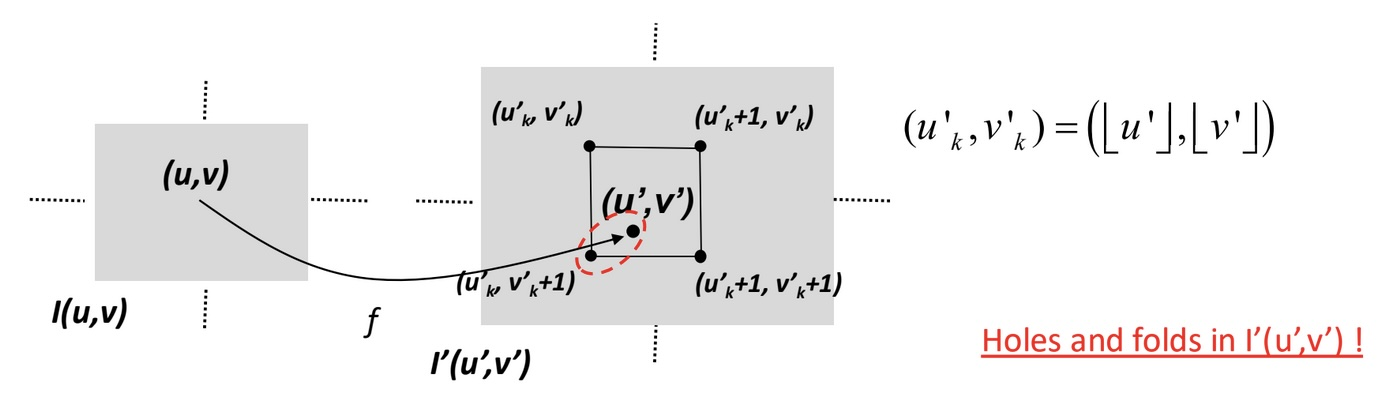
\includegraphics[width=0.8\linewidth]{./img/forward_mapping.jpg}
  \caption{A better choice consists in mapping to the closest point into the destination image}
  \label{fig:forward_mapping}
\end{figure}

Since the coordinates are always real values the different mapping strategies can be to map the closest point or to interpolate between the 4 closest points.

\vspace{3em}
\section{Advanced Topics in Deep Learning for Computer Vision}

\subsection{Recall on CNNs}

In representation learning we try to find good ways of representing data, often by learning a useful transformation of the raw data.
Deep learning is a subset of representation learning.

\subsubsection{Gradient descent}
Neural networks are usually trained using iterative, gradient-based optimizers that drive the cost function to a very low value.
The convergence point of gradient descent depends on the initial values of the parameters.
For feedforward neural networks it's important to initialize all weights to small random values and to initialize biases to zero or to small positive values.
To apply gradient based learning we must choose a cost function and how to represent the output of the model.
The derivative $f'(x)$ gives the slope of $f(x)$ at the point $x$.
The derivative is useful for minimizing a function because it tells us how to change $x$ in order to make a small improvement in $y$.
A point that obtains the absolute lowest value of $f(x)$ is a global minimum.

To reach the minimum we use the formula $w' = w - \alpha \frac{\partial J(w,b)}{\partial w} \,\, b' = b - \alpha \frac{\partial J(w,b)}{\partial b}$, where $\alpha$ is the learning rate, which controls how big are the steps that we take during the gradient descent.
If the slope is positive, we subtract the quantity in order to reach the minimum, or else we do the opposite thing.

As the training set size grows to billions of examples, the time to take a single gradient step becomes prohibitively long.
Stochastic/Minibatch gradient descent are extensions of the gradient descent algorithm. We can sample a minibatch of examples drawn uniformly from the training set (1 for stochastic).
It's like training every time on a different (smaller) training set.

\paragraph{Optimizers: momentum}
Momentum was designed to accelerate learning, especially in the face of high curvature, small but consistent gradients, or noisy gradients.
The size of the step depends on how large and how aligned a sequence of gradients are.
The step size is largest when many successive gradients point in the same direction.
Momentum smooths the step of the gradient descent in its path to the minimum.
We compute: $W^{[l+1]} = W^{[l]} - \alpha v_{W^{[l + 1]}}$, where $v_{W^{[l + 1]}} = \beta v_{W^{[l]}} + (1-\beta) \frac{\partial J(...)}{\partial W^{[l]}}$.
Root Mean Square Propagation (RMSprop) uses an exponentially decaying average to discard history from the extreme past so that it doesn't impede the convergence.

\paragraph{Optimizers: Adam}
The name derives from "adaptive moments", and it can be seen as the combination of RMSprop and momentum.
It's fairly robust to the choice of hyperparameters, though the learning rate sometimes needs to be changed from the suggested default.
There is a first order and a seond order Adam.
The first order Adam uses the gradient and its moving averages (first moments) to update the parameters.
The second order Adam incorporates information about the curvature of the loss surface, using approximations of the Hessian or second order derivatives, which leads to more informed and potentially more efficient updates but requires more computational resources.

\subsubsection{Convolutions and filters}
An image is characterized by height, width and number of channels.

\begin{figure}[htbp]
  \centering
  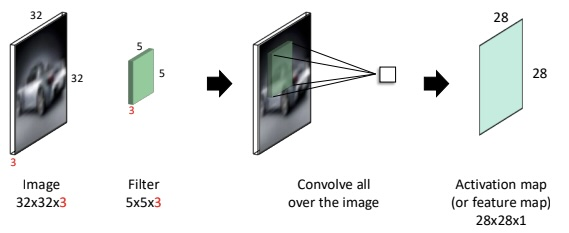
\includegraphics[width=0.8\linewidth]{./img/convolution_filter.jpg}
  \caption{A convolutional filter has the \textbf{same depth} of the input volume, so the output dimension is 1.}
  % \label{fig:forward_mapping}
\end{figure}

We can also train more than one filer, where each filter outputs a feature map.
By stacking activation maps we get a new volume.

Since convolutions shrink the images we can use padding to preserve the edges.
We have always considered a stride of 1 (moving the convolutional filter by one pixel), but we can also use different stride sizes to shrink the image.

\begin{figure}[htbp]
  \centering
  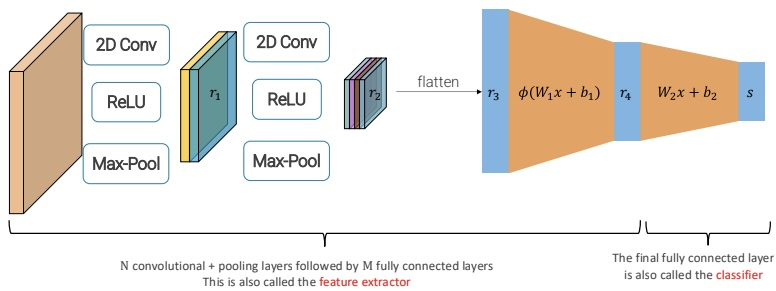
\includegraphics[width=0.8\linewidth]{./img/deep_cnn.jpg}
  \caption{By stacking together convolutional filters, pooling layers and fully connected layers we can design a Deep CNN.}
\end{figure}

\paragraph{Pooling}
A pooling layer is used to reduce the size of the representation in order to speedup computation.
Pooling comes usually after each conv layer or after a block (or set) of conv layers.
It's applied to each activation map independently.

\begin{figure}[htbp]
  \centering
  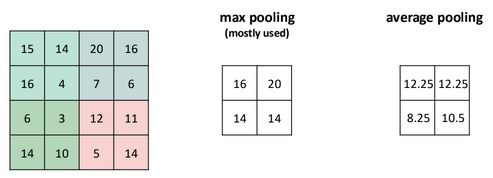
\includegraphics[width=0.8\linewidth]{./img/pooling.jpg}
  \caption{Example: pooling of dimension 2 and stride 2.}
\end{figure}

\paragraph{Receptive fields}
The input pixels affecting a hidden unit are called its receptive field.
We can encode the information in all the pixels to a single point.
We go from spatial to semantic information (we transform spatial information to semantic information).

\paragraph{Convolution parameters and flops}

\begin{figure}[htbp]
  \centering
  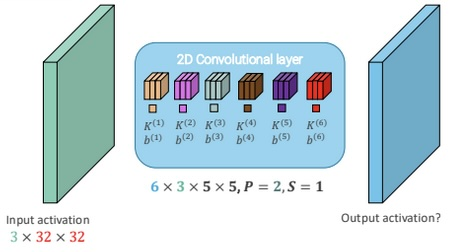
\includegraphics[width=0.8\linewidth]{./img/convolutions_flops.jpg}
  \caption{}
  \label{fig:convolutions_flops}
\end{figure}

As we can see in \ref{fig:convolutions_flops}, the number of learnable parametes for the convolutional layer is $6 \times (3 \times 5 \times 5 + 1) = 6 \times 76 = 456$ (6 convolutional blocks, 3 channels per convolutional block, $5 \times 5$ convolution, ).
The size of the output is $H_\text{{out}} = W_\text{{out}} = 32 - 5 + 2 * 2 + 1 = 32$.
Hence, there are $6 \times 32 \times 32 = 6144$ values in the output activation ($\approxeq 24$KB).

Since each of them is obtained as the dot product between the weights and the input, which requires to perform $n$ multiplications and $n$ summations for inputs of size $n$, i.e. $2n$ flops.

\subsubsection{Batch Normalization (BatchNorm)}
BatchNorm is a technique designed to stabilize and accelerate the training of deep neural networks by addressing internal covariate shift: the change in the distribution of layer activations caused by updates to preceding layers during training.
By normalizing activations at each layer, BatchNorm ensures that gradients are propagated more effectively, enabling coordinated updates across deep networks.

Let $Z^{[l]}$ be a minibatch of activations of the $l$-th layer to be normalized.
To normalize $Z^{[l]}$, we replace it with: $Z^{[l]}_{norm} = \frac{Z^[l] - \mu}{\sigma}$, where $\mu$ is a vector containing the mean of each unit and $\sigma$ is a vector containing the mean of each unit and $\sigma$ is a vector containing the standard deviation of each unit.
$\mu$ and $\sigma$ are running averages of the values seen during training.
BatchNorm helps with speeding up the training, and has a slight regularization effect (but we don't use it for this reason).

We use LayerNorm for fully connected layers because it normalizes per sample, making it batch-size independent.
We use InstanceNorm for convolutional layers because it normalizes per sample and per channel.

\subsubsection{Dropout regularization}
Dropout randomly deactivates a fraction of neurons during training, effectively training an ensemble of smaller sub-networks.
For each layer, you set a dropout probability, determining the chance a neuron is ignored in a forward pass.
This helps to prevent overfitting because we don't associate a certain pattern to a certain output of the network.

\begin{figure}[htbp]
  \centering
  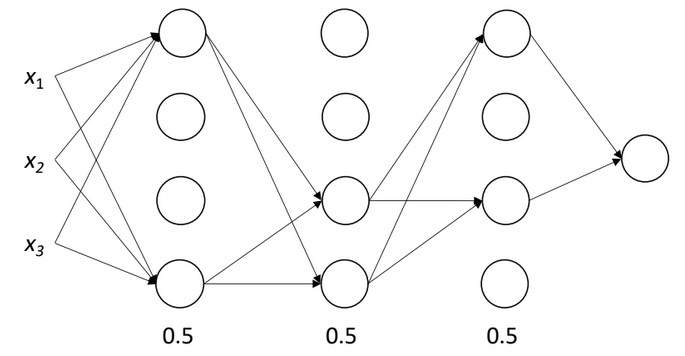
\includegraphics[width=0.8\linewidth]{./img/dropout.jpg}
  \caption{Each layer has a $50 \%$ dropout probability}
  \label{fig:dropout}
\end{figure}

Dropout and normalization are used only at training time.
When we test the network we switch off dropout and regularization.

Another powerful regularization technique is just having more data.

\subsubsection{Data augmentation}
We can create more data by modifying the images we already have.
We must only make transformations which keep the labels valid.
We can, for example, sample random crops/scales of the data or do color augmentation.

Cutout is the process where we remove a random square region of the input image.
This forces the network to use a more diverse set of features, helping generalization.
It's gray because we subtract the mean from this pictures, and so the number in the cutout becomes 0.

\subsection{CNNs}

\subsubsection{AlexNet \& ZFnet}
In 2012 Alex Krizhevsky proposed AlexNet, which had almost a $9\%$ of improvement on SOTA.

\begin{figure}[htbp]
  \centering
  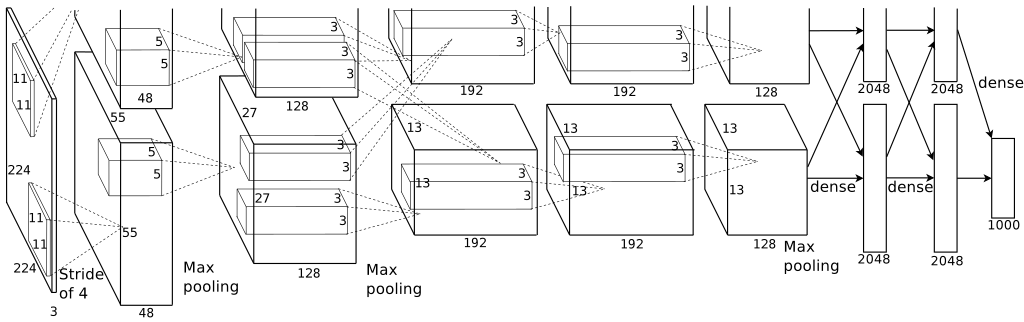
\includegraphics[width=0.8\linewidth]{./img/alexnet.png}
  \caption{AlexNet architecture}
  \label{fig:alexnet}
\end{figure}

In the image \ref{fig:alexnet}, we see only one half of the network, since the architecture is replicated identically 2 times to be used on a 2 GPU setup.
The network is composed by a \textbf{stem layer} at the beginning, which is a convolution layer that performs a fast reduction in the spatial size of the activations, mainly to reduce memory and computational cost.
The first layer has two $11 \times 11$ kernels, which extracts corners/edges/blobs.

To counteract these problems ZFnet used $7\times 7$ convolutions with stride 2 in the first layer and $5\times 5$ convolutions with stride 2 also in the second convolutional layer.

\subsubsection{VGG}
To avoid the vanishing gradient problem VGG used $3 \times 3$ convolutions only, and didn't use the stem layer.
The network was shallower, and used only convolutions and pooling.
At the end it used the same flattening and classification head.

Pre initialization with weights from shallower architectures was crucial to let the training progress, since batch normalization wasn't yet invented.

\begin{figure}[htbp]
  \centering
  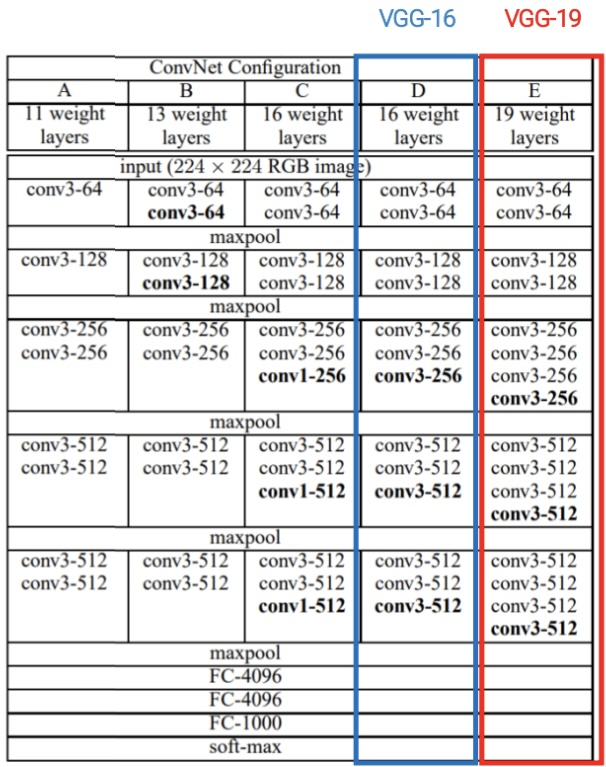
\includegraphics[width=0.35\linewidth]{./img/vgg.jpg}
  \caption{VGG architecture}
  % \label{fig:alexnet}
\end{figure}

VGG introduces the idea of designing a network as repetition of stages, i.e. a fixed combination of layers that process activations at the same spatial resolution.
In VGG we have 3 types of blocks:
\begin{itemize}
  \item \verb|conv-conv-pool|.
  \item \verb|conv-conv-conv-pool|.
  \item \verb|conv-conv-conv-conv-pool| (we can get a more complex convolution by combining $3\times 3$ convolutions).
\end{itemize}

One stage has the same receptive field of larger convolutions but requires less parameters and computation, and introduces more non-linearities.

The disadvantage is that the memory for activation doubles.

\begin{table}[htbp]
\begin{tabular}{|l|l|l|l|l|}
\hline
convolutional layer                                    & params       & flops                 & ReLUs & number of activations                \\ \hline
$C \times C \times 5 \times 5, \,S=1,\, P=2$           & $25C^2 + C$  & $50C^2 W_{in} H_{in}$ & 1     & $C\times W_{in} \times H_{in}$ \\ \hline
2 stacked $C \times C \times 3 \times 3, \,S=1,\, P=1$ & $18C^2 + 2C$ & $10C^2 W_{in} H_{in}$ & 2     & $2\times C \times W_{in} \times H_{in}$ \\ \hline
\end{tabular}
\end{table}

VGG-16 is composed by 138M parameters ($2.3x$ AlexNet), mostly in fully connected layers.
The computational cost is $\approx 4$ Tflops, mainly due to convolutions, and the network uses about $\approx 16.5$ GB of memory.

\subsubsection{Inception v1 (GoogLeNet)}
The main hallmark of this architecture is the improved utilization of the computing resources inside the network.
This was achieved by a carefully crafted design that allows for increasing the depth and width of the network while keeping the computational budget constant.

\begin{figure}[htbp]
  \centering
  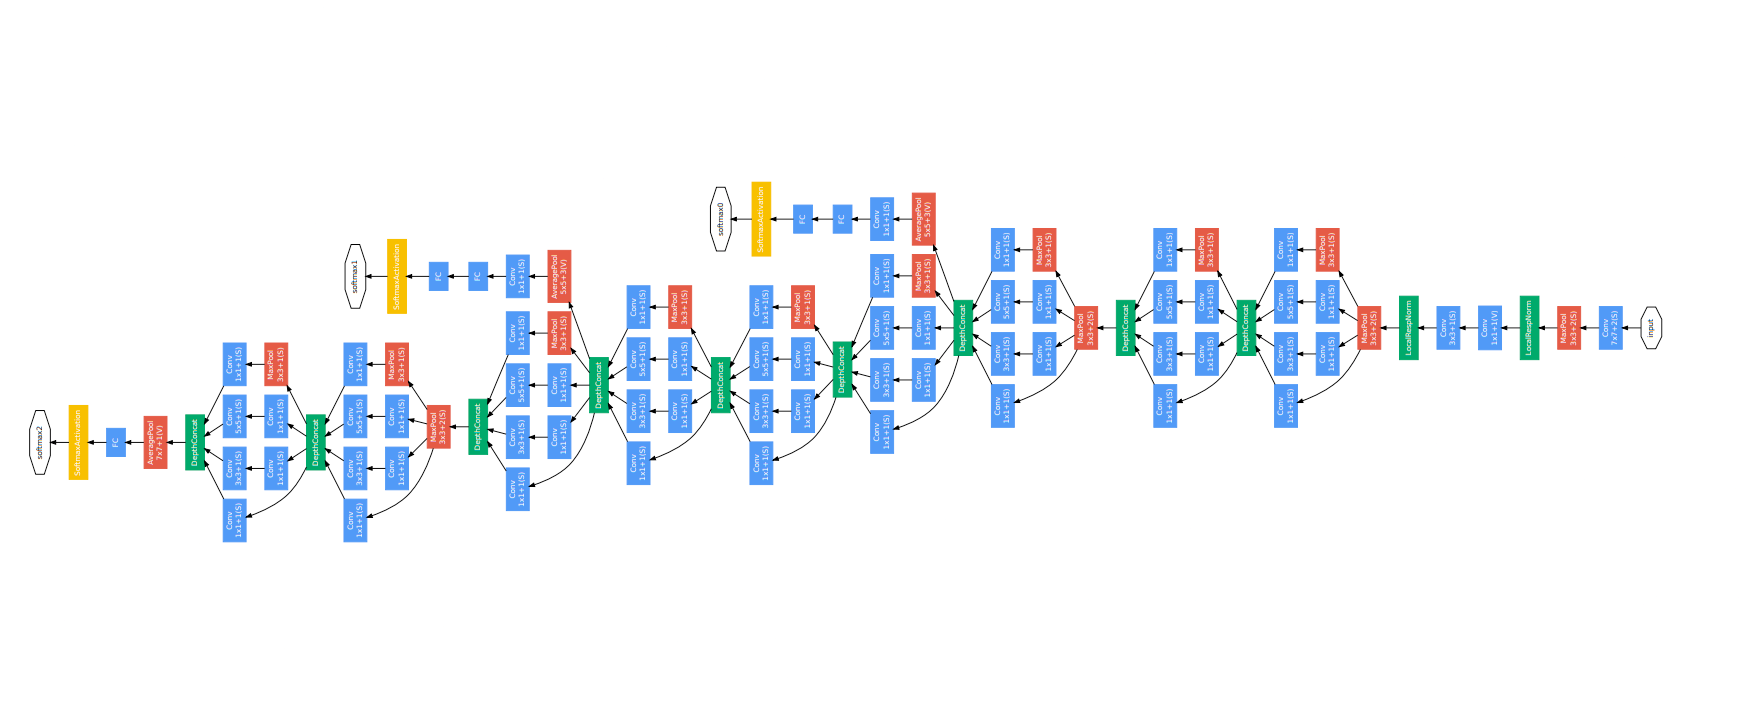
\includegraphics[width=0.99\linewidth]{./img/googlenet.png}
  \caption{GoogLeNet architecture}
\end{figure}

The network is composed by stem layers which shrink the image size, a stack of inception modules where a combination of different operations are combined, and a final classifier.
There are 22 trainable layers and about 100 modules (the blue and red blocks).

\paragraph{Stem layers}
Stem layers aggressively downsamples inputs: from 224 to 28 width/height in 5 layers.
It brings it down a bit more gently than AlexNet.
To reach $28\times 28$, VGG uses 10 layers.

\paragraph{Naïve inception module}
The main idea of the inception module is that it consists of multiple pooling and convolution operations with different sizes ($3\times 3$, $5\times 5$) in parallel, instead of using just one filter of a single size.
\begin{figure}[htbp]
  \centering
  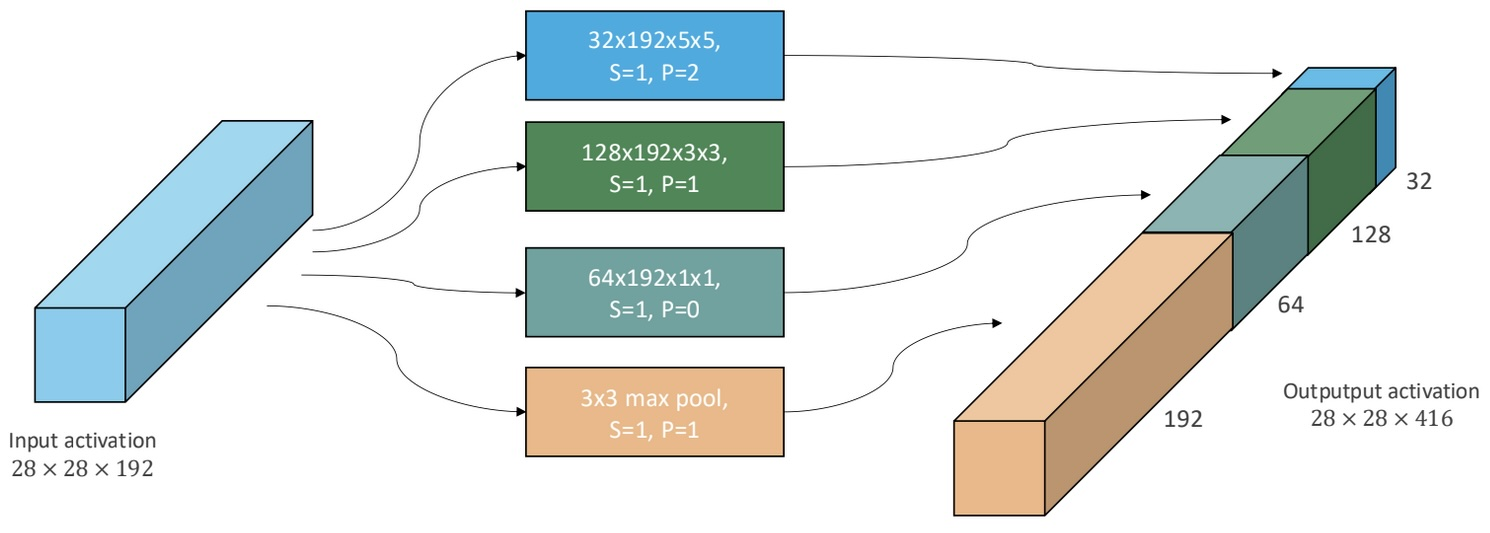
\includegraphics[width=0.8\linewidth]{./img/inception_naive.jpg}
  % \caption{}
\end{figure}
However, there are two main problems:
\begin{itemize}
  \item Due to max-pool, the number of channels grows very fast when inception modules are stacked on top of each other.
  \item $5 \times 5$ and $3 \times 3$ convolutions on many channels become prohibitively expensive if we stack a lot of them.
\end{itemize}

\paragraph{$1 \times 1$ convolutions and the inception module}
To overcome the problems, we use $1 \times 1$ convolutions before feeding the data into $3\times 3$ or $5 \times 5$ convolutions.
$1\times 1$ convolutions don't reason locally, but along the channel on a single dimension.
They allow us to change the depth of the activations while preserving the spatial size.
This is effectively a dimensionality reduction.

\begin{figure}[htbp]
  \centering
  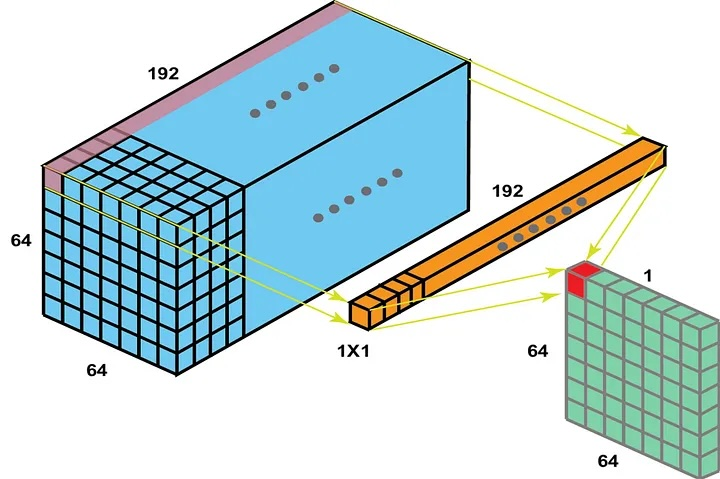
\includegraphics[width=0.8\linewidth]{./img/11conv.jpg}
  \caption{$1 \times 1$ convolution}
\end{figure}

By adding $1\times 1$ convolutions before larger convs and after max pool we can:
\begin{itemize}
  \item \textbf{Control the time complexity} of the larger convolutions by reducing the channel dimension.
  \item \textbf{Control the number of output channels} by reducing the depth of the max pool output.
\end{itemize}

\begin{figure}[htbp]
  \centering
  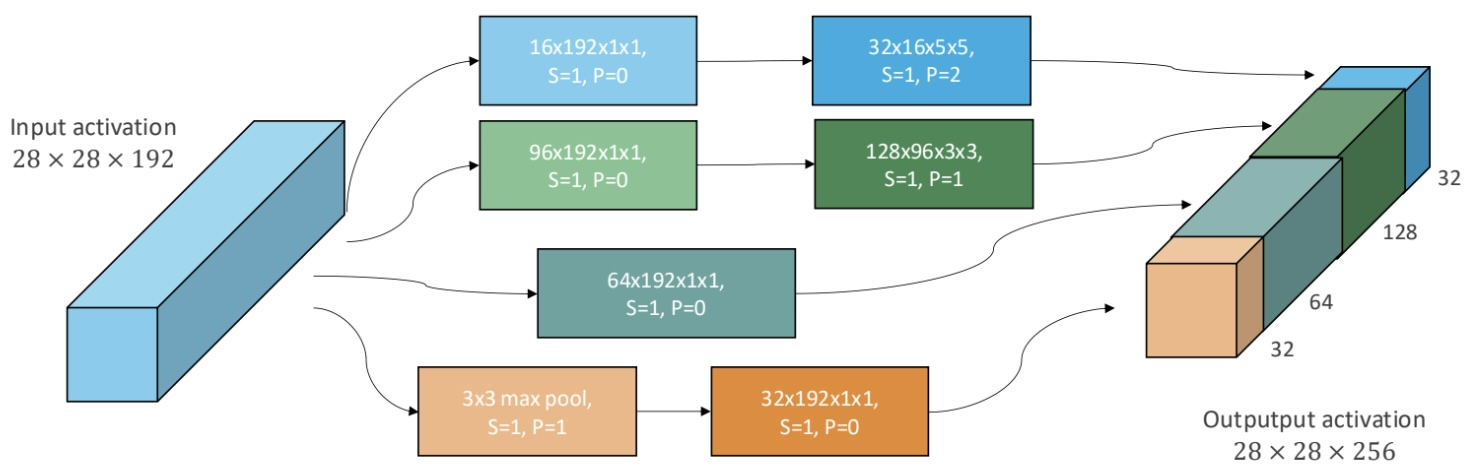
\includegraphics[width=0.8\linewidth]{./img/inception.jpg}
  \caption{Inception module in GoogLeNet}
  \label{fig:inception}
\end{figure}

In \ref{fig:inception} we can see how Google exploited the properties of $1\times 1$ convolutions to make an incpetion module without making the complexity explode.
The idea is that we take our input, we shrink it by using $1\times 1$ convolutions, and then we apply the $5 \times 5$ and $3 \times 3$ spatial convolutions.
We use $1\times 1$ convolutions \textbf{after} pooling to shrink the output (we don't need to compress before the operation but after it).

\paragraph{Fully-connected classifier vs global average pooling}
As we have seen the last 3 fully connected layers were the heaviest, since we had very high dimensional spatial information.
To reduce the number of parameters needed between convolutional features and fully connected layers we get rid of spatial dimensions by averaging them out, because the activations should contain high level information.

\subsubsection{Inception v3}
Inception v3 leverages convolution factorizations to increase the computational efficiency and to reduce the number of parameters, the two main methods are:
\begin{itemize}
  \item $3 \times 3$ followed by $3 \times 3$ instead of a $5 \times 5$ (VGG idea).
  \item $3 \times 3$ can be factorized in a $3\times 1$ and $1 \times 3$.
\end{itemize}

\begin{figure}[htbp]
  \centering
  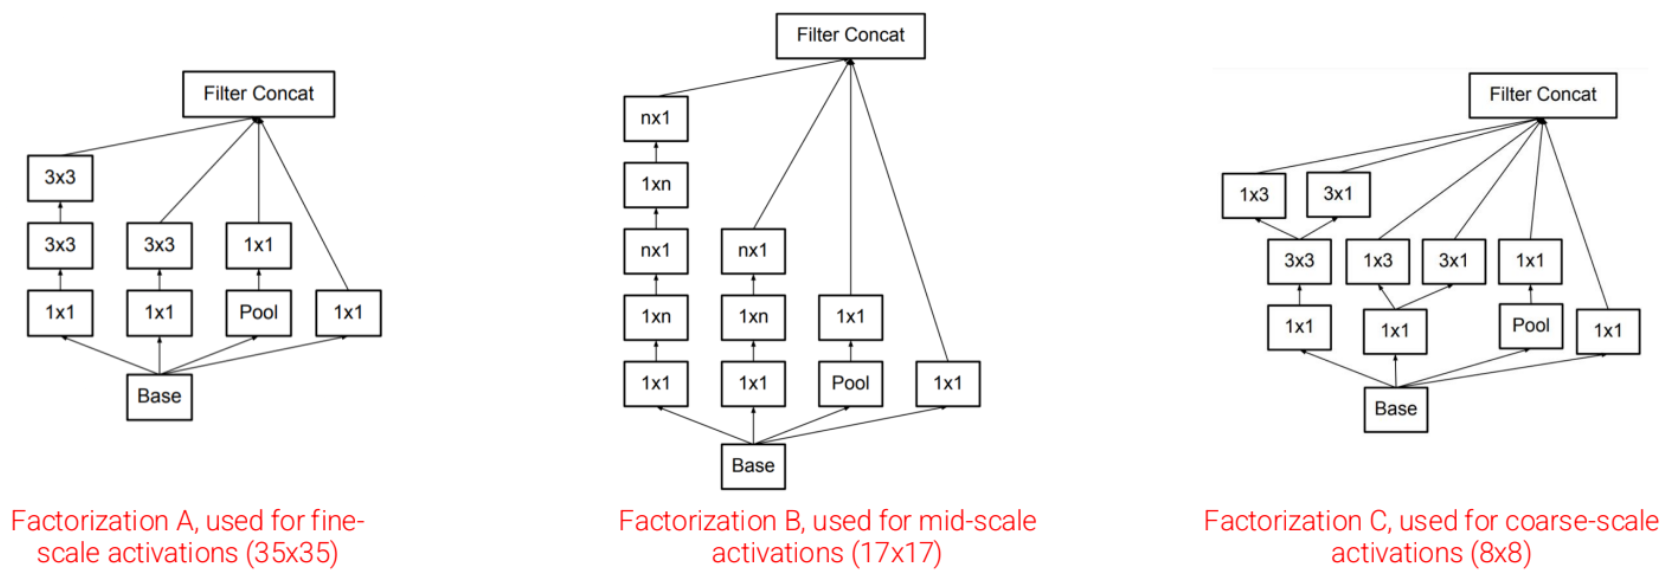
\includegraphics[width=0.8\linewidth]{./img/inception3.png}
  \caption{Instead of always using the same inception layers, we use 3 different inception layers}
\end{figure}

\subsubsection{Residual Networks (ResNet)}
ResNet was invented to address the problem of vanishing gradients and degradation in very deep neural networks.
The core innovation in ResNet is the residual block, which introduces skip connections.
In traditional networks, each layer feeds directly into the next layer.
In ResNet, the input to a layer is also added to its output, by creating what's called a skip connection (like an identity shortcut).
This means that instead of learning a direct mapping $H(x)$, the network learns the residual function $F(x) = H(x) - x$.

\begin{figure}[htbp]
  \centering
  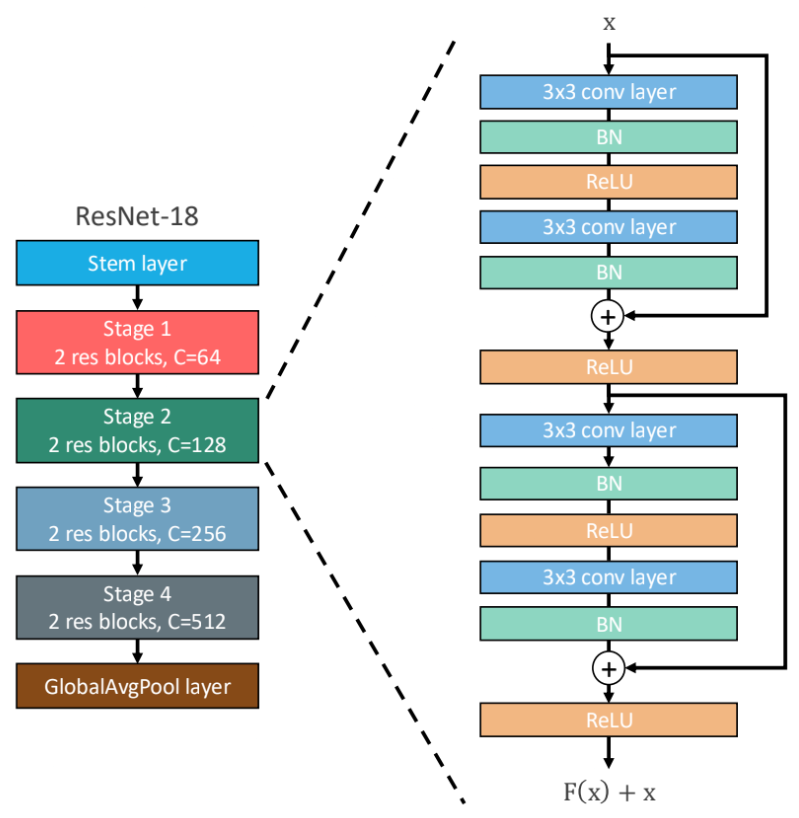
\includegraphics[width=0.8\linewidth]{./img/resnet.png}
  \caption{The ResNet architecture}
\end{figure}

The network is a stack of stages with fixed design rules (inspired by VGG):
\begin{itemize}
  \item Stages are a stack of residual blocks.
  \item Each residual block is a stack of two $3 \times 3$ convolutions with batch-norm.
  \item The first block of each stage halves the spatial resolution (with stride 2 convolutions) and doubles the number of channels.
  \item It uses stem layer and global average pooling as GoogLeNet.
\end{itemize}

\begin{figure}[htbp]
  \centering
  \includegraphics[width=0.8\linewidth]{./img/resnet_skip.png}
  % \caption{}
\end{figure}

ResNet is still the standard baseline for most tasks today.

The residual blocks described so far \textbf{cannot be used as the first block of a new stage}, because the number of channels and the spatial dimensions do not match along the residual connection.
The authors then decided to use a $1\times 1$ convolution with stride 2 and $2C$ output channels to expand the dimension of the channels.

\paragraph{Bottleneck residual block}
A bottleneck residual block is a design used in very deep ResNets (e.g. ResNet-50, 101, 152) to enable training with more layers while maintaining computational efficiency.
\begin{figure}[htbp]
  \centering
  \includegraphics[width=0.8\linewidth]{./img/resnet_bottleneck.png}
  \caption{Instead of working with $3 \times 3$ convolutions we go from $4C$ down to $C$ and then expand again}
\end{figure}

\subsubsection{ResNeXt}
Inception modules are effective multi-branch architectures, which can be thought of as following a split-transform-merge paradigm.
ResNeXt is a simpler way to realize multiple pathways, since it decomposes each bottleneck residual block of ResNets into $G$ parallel branches.
The number of branches (cardinality) is a new hyperparameter.
Once $G$ is chosen, it is possible to obtain a $G \times d$ ResNeXt block with complexity similar to the original ResNet block.
$d$ must be proportional to $C$.

\paragraph{ResNeXt block as grouped convolutions}

Grouped convolutions split input channels into $G$ independent groups.
Each group processes a subset of channels, reducing computational cost and parameters while maintaining feature diversity.

\begin{figure}[htbp]
  \centering
  \includegraphics[width=0.8\linewidth]{./img/grouped_convolutions.jpg}
  \caption{Grouped convolution with $G=2$}
\end{figure}

An input with $C$ channels is divided into $G$ groups, each with $\frac{C}{G}$ channels.
Each group has its own filters, producing $\frac{K}{G}$ output channels (for $K$ total filters).
The outputs are concatenated, resulting in $K$ channels.

This is useful because it's more efficient and each group learns distinct features, enhancing model capacity.

ResNeXt introduces cardinality (the number of groups of $G$) as a new dimension.
It uses grouped convolutions to create parallel pathways within a residual block, improving feature learning without increasing depth/width.

\begin{figure}[htbp]
  \centering
  \includegraphics[width=0.8\linewidth]{./img/resnext_grouped.jpg}
  \caption{The ResNeXt block as grouped convolutions, on the left we have a normal convolutional block, in the middle we split to reduce computation and on the right we join again.}
\end{figure}

The structure of the ResNeXt block is:
\begin{itemize}
  \item $1\times 1$ convolution to compress the input channels.
  \item $3\times 3$ grouped convoltuion to process compressed features in $G$ parallel groups (cardinality). Each group applies transformations independently.
  \item $1\times 1$ convolutions expands channels back.
  \item skip connection adds the original input to the output (residual learning).
\end{itemize}

ResNeXt is more efficient because there are fewer parameters than widening/deepening the network, and by increasing $G$ we can improve the performance without drastically increasing the compute.

\subsubsection{Squeeze-and-Excitation Networks (SENet)}
It's the last paper which won CVPR.
It proposed the squeeze-and-excitation module to capture global context and to use it to reweight channels in each block.
Given the output $U$ of a block with shape $C \times H \times W$ we do:
\begin{itemize}
  \item Global average pooling to squeeze.
  \item General bottleneck formed by two fully connected layers with reduction ratio 16.
\end{itemize}

\begin{figure}[htbp]
  \centering
  \includegraphics[width=0.8\linewidth]{./img/senet.jpg}
  \caption{SENet block diagram}
\end{figure}

\subsubsection{Depthwise Separable convolutions}
F. Chollet one year after the SENet paper proposed the Depthwise Separable convolutions.
The standard convolutions filter features based on the convolutional kernels and combine features in order to produce new representations.
This is very expensive.
Depthwise separable convolutions separates filtering and combination, and this aggressively limits the computational cost.

\begin{figure}[htbp]
  \centering
  \includegraphics[width=0.8\linewidth]{./img/separable_convolution.png}
  % \caption{}
\end{figure}

\subsubsection{Inverted residual blocks}
MobileNet-v2 introduced the bottleneck residual block to scale up the model depth by increasing the number of layers per block while keeping the computation and number of parameters roughly constant.
To this end, it uses a pair of $1\times 1$ convolutions, where the first compresses the number of channels, while the second one expands them.
Hence, the $3\times 3$ convoltuion operates in the compressed domain.

\begin{figure}[htbp]
  \centering
  \includegraphics[width=0.8\linewidth]{./img/bottleneck_residual.jpg}
  % \caption{}
\end{figure}

As we know, compression usually results in information loss, so in MobileNet-v2 inverted residual blocks were proposed.
In this blocks, the first $1\times 1$ convolution expands the channels, while the second compresses them back, according to an expansion ratio $t$.
To limit the increase in computation, the inner $3\times 3$ convolution is realized as a depthwise convolution (single filter per input channel instead of applying the filters across all the input channels).

\begin{figure}[htbp]
  \centering
  \includegraphics[width=0.8\linewidth]{./img/inverted_residual.jpg}
  % \caption{}
\end{figure}

\subsubsection{MobileNet-v2}
MobileNet-v2 is a stack of inverted residual blocks with ReLUs in between.
The number of channels grows slowly compared to previous architectures, as we can see in the purple rectangle in figure \ref{fig:mobilenet}

\begin{figure}[htbp]
  \centering
  \includegraphics[width=0.8\linewidth]{./img/mobilenet.jpg}
  % \caption{}
  \label{ref:mobilenet}
\end{figure}

Whenever spatial dimensions or number of channels do not match between input and output, there are no residual connections.

\subsubsection{EfficientNet}
EfficientNet proposed to design the network based on resources.
As we know there are 3 dimensions for scaling a neural network: width, depth and resolution.

\begin{figure}[htbp]
  \centering
  \includegraphics[width=0.8\linewidth]{./img/efficientnet.jpg}
  \caption{Different types of NN scaling.}
\end{figure}

Bigger networks with larger width, depth or resolution tend to achieve higher accuracy, but the accuracy gain quickly saturates after reaching $80 \%$, which is a limitation of single dimenison scaling.
\textbf{Scaling dimensions are not independent}. Intuitively, for higher resolution images, we should increase network depth, such that the larger receptive fields can help to capture similar features that include more pixels in bigger images.
Correspondingly, we should also increase netowrk width when the network resolution is higher, in order to capture more fine-grained patterns with more pixels in high resolution images.

EfficientNet  uses a compound coefficient $\phi$ to scale all dimensions in a principled way.

\subsection{RNNs \& Transformers}

In RNNs, which were used to avoid the problem of fixed size input, the gradient computetion involves performing a forward propagation pass moving from left to right through the unrolled graph of the network, followed by a backward propagation pass moving right to left through the graph.
The basic problem is that by propagating the gradient over many stages it tends to vanish or explode, so learning long-term dependencies can take a lot of time.

\paragraph{Encoder-Decoder architecture}
In this type of architecture the encoder processes the input sequence.
It emits the context $C$, usually as a function of its final hidden state.
The decoder is conditioned on that fixed-length vector to generate the output sequence.
If the context $C$ is a vector, then the encoder RNN is simply a sequence-to-vector RNN, and the decoder is a vector-to-sequence RNN.
The \textbf{bottleneck problem} arises because the context $C$ outputted by the encoder RNN has a dimension that is too small to properly summarize a long sequence.

\paragraph{Attention}
Existing model for neural machine translation encode a source sentence into a fixed-length vector from which a decoder generates a translation.
Attention provides a solution to the bottleneck problem. 
We provide to the decoder the learned token start, then we do the dot product between the start token and the hidden states.
All the other hidden states give us a probability for each token.

\begin{figure}[htbp]
  \centering
  \includegraphics[width=0.8\linewidth]{./img/rnn_classic.png}
  \caption{In the classic RNN, the last hidden state is used for all the translation.}
\end{figure}

\begin{figure}[htbp]
  \centering
  \includegraphics[width=0.8\linewidth]{./img/attention.png}
  \caption{In the attention mechanism, at each step, the current hidden state is compared with all the previous hidden states by computing an attention score.}
\end{figure}

\subsubsection{Transformer architecture}
The inherently sequential nature of RNN precludes parallelization within training examples, which becomes critical with longer sequence lengths.
The \textbf{transformer} is the first model relying entirely on self-attention (and cross-attention) to compute representations of its input and output without using RNNs or convolutions.
It's still an encoder-decoder architecture, where the encoder maps an input sequence of symbol representations $(x_1, ..., x_n)$ to a sequence of continuous representations $z=(z_1, ..., z_n)$.
Given $z$, the decoder generates an output sequence $(y_1, ..., y_m)$ of symbols one element at a time.
At each step the model is \textbf{auto-regressive}, consuming the previously generated symbols as additional input when generating the next.

\begin{figure}[htbp]
  \centering
  \includegraphics[width=0.6\linewidth]{./img/transformer.jpg}
  \caption{The transformer architecture from the paper "Attention is all you need".}
\end{figure}

\paragraph{Transformer encoder}
In the encoder we turn each input word into a vector by using an embedding layer.
Each word is embedded into a vector of size $d_{\text{model}}$.
If the encoders are stacked, the embedding only happens in the bottom-most encoder.
Since we process the words in parallel we lose positional information, so by using positional encoding we keep this information.
The positional encoding has the same dimension $d_{\text{model}}$ as the embeddings, so that the two can be summed.
There are learned and fixed positional encodings; the authors used sine and cosine functions of different frequencies.

Each layer has two sub-layers:
\begin{itemize}
  \item A multi-head self attention mechanism.
  \item A fully connected feed-forward network. The exact same feedforward network is independently applied to each position (shared parameters).
\end{itemize}

There is also a residual connection around each of the two sub-layers, followed by layer normalization.
To facilitate these residual connections, all sub-layers in the model, as well as the embedding layers, produce outputs of dimension $d_{\text{model}}$.

\paragraph{Transfromer decoder}
The decoder is also composed of a stack of $N$ identical layers.
In addition of the two sub-layers of the encoder, the decoder has a third sub-layer, which performs multi-head attention over the output of the encoder stack (cross-attention).
As in the encoder tehre are residual connections and layer normalization.

The self-attention sub-layer in the decoder stack is modified so as to \textbf{prevent positions from attending to subsequent positions}.
This masking, combined with the fact that the output embeddings are offset by one position, ensures that the predictions for position $i$ can depend only on the known outputs at positions less than $i$.

\paragraph{Self-Attention}
The first setp in calculating self-attention is to create three vectors from each of the embedded words:
\begin{itemize}
  \item a Query vector.
  \item a Key vector.
  \item a Value vector.
\end{itemize}

These vectors are created by multiplying the embeddings by three matrices learned during the training process.
Their dimensionality is $d_k = \frac{d_{\text{model}}}{h}$, while the embedding and encoder input/output vectors have dimensionality of $d_{\text{model}}$.

The matrices are used to compute the self-attention score.
$$\text{Attention}(Q,K,V)=\text{softmax}(\frac{QK^T}{\sqrt{d_k}})V$$

As we can see there is a little normalization done with $\sqrt{d_k}$, to try to avoid having the results of the softmax squeezed too much into a single value (one hot).
The scores of the self-attention determine how much focus to place on other parts of the input sentence as we encode a word at a certain position.

\paragraph{MultiHead Attention}
The purpose of multi-head attention is to linearly project the queries, keys and values $h$ times with different, learned linear projections.
On each of these projected versions of queries, keys, and values we perform the attention function in parallel.
The outputs of different heads are then concatenated and once again projected.
Multi-head attention allows the model to jointly attend to information from different representation subspaces at different positions.

\paragraph{Multi Head Self-Attention computation}

\paragraph{Cross-Attention}
in the cross attention layers, the queries come from the previous decoder layer (masked self-attention), and the keys and values come from the output of the encoder.
This allows every position in the decoder to attend over all positions in the input sequence.
It's a very powerful mechanism used in modern generative models to introduce variable lengths conditions.


\subsubsection{Vision Transformer (ViT)}
We split an image into patches and provide the sequence of linear embeddings of these patches as an input to a Transformer.
The image patches are treated the same way as tokens in an NLP application.

As an alternative to raw image patches, the input sequence can be formed from feature maps of a CNN.
In this hybrid model, the patch embedding projection is applied to patches extracted from a CNN feature map.

To handle $2D$ images, we reshape the image $x \in \mathbb{R}^{H\times W \times C}$ into a sequence of flattened $2D$ patches $x_p \in \mathbb{R}^{N \times (P^2 \cdot C)}$.
\begin{itemize}
  \item $(H, W)$ is the resolution of the original image.
  \item $C$ is the number of channels.
  \item $(P, P)$ is the resolution of each image patch.
  \item $N = \frac{HW}{P^2}$ is the resulting number of patches, which also serves as the effective input sequence length for the transformer.
\end{itemize}

The transformer uses constant latent vector size $d_{\text{model}}$ through all of its layers, so we flatten the patches and map to $d_{\text{model}}$ dimensions with a trainable linear projection.
We also prepend a learnable embedding to the sequence of embedded patches, whose state at the output of the transfromer encoder serves as the image representation.
The classification head is implemented by a MLP with one hidden layer.
To retain positional information the ViT uses learnable 1D position embeddings.

At the start, the ViT worked very bad.
This is because transformers lack some of the inductive biases inherent to CNNs, such as translation equivariance and locality, and therefore do not generalize well when trained on insufficient amounts of data.
The convolution in combination with max pooling/striding makes CNNs approximately invariant to translation.
When a module is translation invariant, it means that if we apply translation transformation on the input image the output of the module won't change.
To solve the inductive bias they gave the network so much data that the classes appear anywhere.

\subsection{Object Detection}
Previously, we have done object detection with SIFT, but we were just able to say if the object was in the image, not where it was.
Now we want to do detection by putting a bounding box around the object.
We do this by returning a set of quadruples: $[x, y, h, w, o]_{i=0}^{K}$, where we have the box position, width, height, and class of the output.

The main challenges are the different lengths of the outputs (since we can detect from 0 to $K$ images), the fact that the outputs have both categorical and spatial information, and the fact that the images are usually processed at higher resolution than neural networks for image classification.

\subsubsection{Viola-Jones Object Detector}
It's a general purpose object detection framework, but it has been mainly applied to faces.
We will now see the three main innovations of the algorithm: the AdaBoost algorithm, cascade, and the use of integral images.

\paragraph{AdaBoost algorithm}
A Weak Learner (WL) is a simple classifier whose error is slightly better than random guessing.
Boosting is a way to train and build an ensemble of $M$ weak classifiers to obtain a Strong Learner SL.
After training a weak learner, the examples are re-weighted in order to emphasize those which were incorrectly classifier by the previous weak classifier.

The \textbf{AdaBoost} algorithm steps are:
\begin{enumerate}
  \item Given $N$ training samples $(x^(i), y^(i))$, assign equal weight to each training example $w^(i)=\frac{1}{N}$.
  \item Iterate for $j = 1, ..., M$ weak learners:
  \begin{enumerate}
    \item Fit the best classifier $WL_j$ to the training data by using the current weights.
    \item Compute the weighted error rate $\epsilon_j = \sum_{i:\, x^{(i)} \text{ is missclassified}} w^{(i)}$.
    \item Compute $\beta_j = \frac{1 - \epsilon_j}{\epsilon_j}$.
    \item Updates weights $w^(i) = w^(i)\beta_j$ for wrongly classified examples.
    \item Re-normalize $w^(i)$ to sum to 1.
  \end{enumerate}
  \item The Strong Learner is given by a weighted majority vote $SL(x) = \sum_{j} \ln \beta_j WL_j(x) > 0$, con $\ln \beta_j = \alpha_j$.
\end{enumerate}

The idea is that missclassified examples gain weight, forcing subsequent learners to focus on harder cases.

\paragraph{Haar-like features}
Weak classifiers used to detect faces are simple rectangular filters, composed of 2 to 4 rectangles applied at a fixed position within a $24 \times 24$ patch.
Even with this simple definition there are over $160$ k possible filters in a $24 \times 24$ patch.
AdaBoost is used to select a small subset of the most effective filters.

\paragraph{Dataset}
The dataset consisted of 4916 hand labeled faces, scaled and aligned to a base resolution of $24 \times 24$ pixels.
The non-face windows were collected by selecting random sub-windows from a set of 9500 images which did not contain faces.

\begin{figure}[htbp]
  \centering
  \includegraphics[width=0.6\linewidth]{./img/adaboost.png}
  \caption{The 2 most effective features selected by AdaBoost on the training set.}
\end{figure}

\paragraph{Integral images and fast feature computation}
To speed up the computation of rectangular features, the authors proposed the use of so-called integral images $II$, where $II(i,j) = \sum_{i' \leq i, j' \leq j} I(i', j')$.

We can compute the value of $II(i,j)$ just by looking at the 3 neighbours: $II(i,j) = II(i, j-1) + II(i-1, j) - II(i-1, j-1) + I(i,j)$, where $II$ are the values in the integral image, and $I$ is the value in the original image.

\begin{figure}[htbp]
  \centering
  \includegraphics[width=0.6\linewidth]{./img/integral_images.jpg}
  \caption{$II(1,2) = II(1,1) + II(0,2) - II(0,1) + I(1,2) = 14 + 11 - 5 + 1$}
\end{figure}

With integral images we could have an overflow problem if numbers get too big.

\begin{figure}[htbp]
  \centering
  \includegraphics[width=0.6\linewidth]{./img/integral_filters.png}
  \caption{Rectangular filters can be computed in constant time with integral images}
\end{figure}

\paragraph{Multi-scale sliding window detector}
At test time, the strong classifier is applied to all spatial locations in the image.
Multi-scale detection is necessary, since faces are not necessarily $24\times 24$.
To achieve good performance, about 200 features are used to classify each patch.
Even if each feature can be computed very fast (thanks to integral images) there are still too many windows in an image to achieve real-time performance.

Faces are far less frequent in an image than background regions.
Most of the time is wasted computing a lot of features for background patches.
The key idea is then to reject most of the easy background patches with a simpler classifier which can be ran very fast.

\paragraph{Box overlap}

\begin{figure}[htbp]
  \centering
  \includegraphics[width=0.6\linewidth]{./img/cascade_classifier.png}
  \caption{We use more and more features for face detection classifier after classifier}
\end{figure}

There will be several overlapping detections.
To check if two boxes overlap we measure the Intersection over Union ($IoU$) score: $IoU(BB_i, BB_j) = \frac{|BB_i \cap BB_j|}{|BB_i| + |BB_j| - |BB_i \cap BB_j|}$. $0.75$ corresponds to a good overlap, $0.90$ to a perfect one.
To obtain a single detection out of a set of overlapping boxes we perform Non Maxima Suppression of boxes.
Non Maxima Suppression considers the highest scoring Bounding Box, eliminates all the boxes with overlap greater than a threshold, and repeats this until all the boxes have been tested.

A detection is considered a True Positive if its overlap with the ground truth $BB^{GT}$ is greater than $\rho_{IoU}$.

\subsubsection{Transfer Learning}
If we can assume that only one object is present in the image, object detection simplifies to object localization.
Transfer learning is a technique where a model trained on one task is reused (or "transferred") for a different but related task.
Instead of training a model from scratch, you start with a pre-trained model and fine-tune it for your specific problem.
To solve object detection we can reuse any architecture used in image classification, by adding a regression head for predicting the bounding box.

We can apply a classification CNN as a sliding window detector.
We have to add a background class to discard background patches.
The problem is that there are too many boxes to try, since we have to try lots of positions with different scales and aspect ratios.
The solution is to use region proposals.

\subsubsection{Region proposals}
Region proposal algorithms inspect the image and attempt to find regions of an image that likely contain an object.
The algorithm as a first step oversegments the image into highly uniform regions, and then, based on similarity scores of color, texture and size it iteratively aggregates them.

\begin{figure}[htbp]
  \centering
  \includegraphics[width=0.6\linewidth]{./img/region_proposal.jpg}
  \caption{The 2 most similar regions are grouped together and then new similarities are calculated between the resulting region and its neighbours}
\end{figure}

\subsubsection{R-CNN: Region-based CNN}

Region-based CNN is the first object detector network.
As we can see in \ref{fig:rcnn} we run selective search to get about 2000 proposals, then we anisotropically (not uniformly across all directions) warp these proposals and add some pixels of context into a fixed size, to be able to input them in AlexNet, and for each proposal we get a class and a bounding box correction.

\begin{figure}[htbp]
  \centering
  \includegraphics[width=0.6\linewidth]{./img/rcnn.jpg}
  \caption{R-CNN network architecture}
  \label{fig:rcnn}
\end{figure}

The problem is that since we have 2 different algorithms (one for the region proposal and one for AlexNet) we can't backpropagate through both of them.

\subsubsection{Fast R-CNN}

In the Fast R-CNN architecture showed in \ref{fig:fastrcnn} we can see that the model has been modified to run the first few layers of AlexNet on the original image, apply RoI pooling to crop and warp convolutional features according to proposal, and then run a small per-region network on each region to get the output class and bounding box correction.
This results in a faster networks since we don't have to apply 2000 CNN forward passes per image, but we apply most of the CNN before warping.

\begin{figure}[htbp]
  \centering
  \includegraphics[width=0.6\linewidth]{./img/fastrcnn.png}
  \caption{Fast R-CNN network architecture}
  \label{fig:fastrcnn}
\end{figure}

Fast R-CNN uses the same bounding box correction of R-CNN, but with a smooth L1 loss (equal to L2 near the origin, but smoother elsewhere).

\paragraph{RoI pooling}
The RoIPool layer converts activations inside Region of Interest, corresponding to rescaled Selective Search regions, into activations with fixed spatial dimensions, which are the ones required by the remaining layers of the network.
To do RoI pooling, given a region:
\begin{enumerate}
  \item Snap the region to the grid.
  \item Apply max pooling kernels with approximate size $[H_r/H_o]\times [W_r/W_o]$ and approximate stride $s = [H_r/H_o]\times[W_r/W_o]$.
\end{enumerate}

\begin{figure}[htbp]
  \centering
  \includegraphics[width=0.6\linewidth]{./img/roipool.png}
  \caption{RoI pooling.}
\end{figure}

\subsubsection{Faster R-CNN}

In Fast R-CNN proposals are not learned, so the selective search is slow.
In Faster R-CNN they introduced a RPN (Region Proposal Network), which learns to predict the proposal box and the objectness score.

\begin{figure}[htbp]
  \centering
  \includegraphics[width=0.6\linewidth]{./img/fasterrcnn.png}
  \caption{Faster R-CNN network architecture.}
\end{figure}

\paragraph{Region Proposal Network}

Region Proposal Networks are applied to a small $3\times 3$ window, which is approximately an object sized window in the original image and doesn't correspond to what we see in \ref{fig:rpn}, predicts the objectness and proposal bounding box.

\begin{figure}[htbp]
  \centering
  \includegraphics[width=0.6\linewidth]{./img/rpn.jpg}
  \caption{Region Proposal Network architecture.}
\end{figure}

When the objectness score is low, the localization head produces its output, but it's meaningless and it will be ignored.

\paragraph{Region Proposal Network with anchor}
We can simplify the creation of proposals.
An easier task may be to correct an input proposal, as done in R-CNN.

\begin{figure}[htbp]
  \centering
  \includegraphics[width=0.6\linewidth]{./img/rpn_anchor.jpg}
  \caption{Our proposal here is a fixed scale and aspect-ratio box, known as anchor.}
\end{figure}

Objects have different scales and asepct ratios, so we use several anchors with different scale and aspect ratios.
The RPN predicts $k$ objectness scores and $k$ corrections.

When training RPNs, given an image and a ground truth bounding box if the anchor has a low IoU with all ground-truth boxes in an image, it's considered as background.

In standard Faster-RCNN, the RPN processes only the last activation of the feature extractor, which is a semantically rich signal since it includes higher level features than previous activations, but very coarse in spatial resolution.
Even if small scale anchors are provided, it may miss objects smaller than the grid size.

% slide 62/71

\end{document}
